%% bare_conf_compsoc.tex
%% V1.4b
%% 2015/08/26
%% by Michael Shell
%% See:
%% http://www.michaelshell.org/
%% for current contact information.
%%
%% This is a skeleton file demonstrating the use of IEEEtran.cls
%% (requires IEEEtran.cls version 1.8b or later) with an IEEE Computer
%% Society conference paper.
%%
%% Support sites:
%% http://www.michaelshell.org/tex/ieeetran/
%% http://www.ctan.org/pkg/ieeetran
%% and
%% http://www.ieee.org/

%%*************************************************************************
%% Legal Notice:
%% This code is offered as-is without any warranty either expressed or
%% implied; without even the implied warranty of MERCHANTABILITY or
%% FITNESS FOR A PARTICULAR PURPOSE! 
%% User assumes all risk.
%% In no event shall the IEEE or any contributor to this code be liable for
%% any damages or losses, including, but not limited to, incidental,
%% consequential, or any other damages, resulting from the use or misuse
%% of any information contained here.
%%
%% All comments are the opinions of their respective authors and are not
%% necessarily endorsed by the IEEE.
%%
%% This work is distributed under the LaTeX Project Public License (LPPL)
%% ( http://www.latex-project.org/ ) version 1.3, and may be freely used,
%% distributed and modified. A copy of the LPPL, version 1.3, is included
%% in the base LaTeX documentation of all distributions of LaTeX released
%% 2003/12/01 or later.
%% Retain all contribution notices and credits.
%% ** Modified files should be clearly indicated as such, including  **
%% ** renaming them and changing author support contact information. **
%%*************************************************************************


% *** Authors should verify (and, if needed, correct) their LaTeX system  ***
% *** with the testflow diagnostic prior to trusting their LaTeX platform ***
% *** with production work. The IEEE's font choices and paper sizes can   ***
% *** trigger bugs that do not appear when using other class files.       ***                          ***
% The testflow support page is at:
% http://www.michaelshell.org/tex/testflow/



\documentclass[conference,compsoc]{IEEEtran}
% Some/most Computer Society conferences require the compsoc mode option,
% but others may want the standard conference format.
%
% If IEEEtran.cls has not been installed into the LaTeX system files,
% manually specify the path to it like:
% \documentclass[conference,compsoc]{../sty/IEEEtran}





% Some very useful LaTeX packages include:
% (uncomment the ones you want to load)


% *** MISC UTILITY PACKAGES ***
%
%\usepackage{ifpdf}
% Heiko Oberdiek's ifpdf.sty is very useful if you need conditional
% compilation based on whether the output is pdf or dvi.
% usage:
% \ifpdf
%   % pdf code
% \else
%   % dvi code
% \fi
% The latest version of ifpdf.sty can be obtained from:
% http://www.ctan.org/pkg/ifpdf
% Also, note that IEEEtran.cls V1.7 and later provides a builtin
% \ifCLASSINFOpdf conditional that works the same way.
% When switching from latex to pdflatex and vice-versa, the compiler may
% have to be run twice to clear warning/error messages.






% *** CITATION PACKAGES ***
%
\ifCLASSOPTIONcompsoc
  % IEEE Computer Society needs nocompress option
  % requires cite.sty v4.0 or later (November 2003)
  \usepackage[nocompress]{cite}
\else
  % normal IEEE
  \usepackage{cite}
\fi
% cite.sty was written by Donald Arseneau
% V1.6 and later of IEEEtran pre-defines the format of the cite.sty package
% \cite{} output to follow that of the IEEE. Loading the cite package will
% result in citation numbers being automatically sorted and properly
% "compressed/ranged". e.g., [1], [9], [2], [7], [5], [6] without using
% cite.sty will become [1], [2], [5]--[7], [9] using cite.sty. cite.sty's
% \cite will automatically add leading space, if needed. Use cite.sty's
% noadjust option (cite.sty V3.8 and later) if you want to turn this off
% such as if a citation ever needs to be enclosed in parenthesis.
% cite.sty is already installed on most LaTeX systems. Be sure and use
% version 5.0 (2009-03-20) and later if using hyperref.sty.
% The latest version can be obtained at:
% http://www.ctan.org/pkg/cite
% The documentation is contained in the cite.sty file itself.
%
% Note that some packages require special options to format as the Computer
% Society requires. In particular, Computer Society  papers do not use
% compressed citation ranges as is done in typical IEEE papers
% (e.g., [1]-[4]). Instead, they list every citation separately in order
% (e.g., [1], [2], [3], [4]). To get the latter we need to load the cite
% package with the nocompress option which is supported by cite.sty v4.0
% and later.





% *** GRAPHICS RELATED PACKAGES ***
%
\ifCLASSINFOpdf
  % \usepackage[pdftex]{graphicx}
  % declare the path(s) where your graphic files are
  % \graphicspath{{../pdf/}{../jpeg/}}
  % and their extensions so you won't have to specify these with
  % every instance of \includegraphics
  % \DeclareGraphicsExtensions{.pdf,.jpeg,.png}
\else
  % or other class option (dvipsone, dvipdf, if not using dvips). graphicx
  % will default to the driver specified in the system graphics.cfg if no
  % driver is specified.
  % \usepackage[dvips]{graphicx}
  % declare the path(s) where your graphic files are
  % \graphicspath{{../eps/}}
  % and their extensions so you won't have to specify these with
  % every instance of \includegraphics
  % \DeclareGraphicsExtensions{.eps}
\fi
% graphicx was written by David Carlisle and Sebastian Rahtz. It is
% required if you want graphics, photos, etc. graphicx.sty is already
% installed on most LaTeX systems. The latest version and documentation
% can be obtained at: 
% http://www.ctan.org/pkg/graphicx
% Another good source of documentation is "Using Imported Graphics in
% LaTeX2e" by Keith Reckdahl which can be found at:
% http://www.ctan.org/pkg/epslatex
%
% latex, and pdflatex in dvi mode, support graphics in encapsulated
% postscript (.eps) format. pdflatex in pdf mode supports graphics
% in .pdf, .jpeg, .png and .mps (metapost) formats. Users should ensure
% that all non-photo figures use a vector format (.eps, .pdf, .mps) and
% not a bitmapped formats (.jpeg, .png). The IEEE frowns on bitmapped formats
% which can result in "jaggedy"/blurry rendering of lines and letters as
% well as large increases in file sizes.
%
% You can find documentation about the pdfTeX application at:
% http://www.tug.org/applications/pdftex





% *** MATH PACKAGES ***
%
%\usepackage{amsmath}
% A popular package from the American Mathematical Society that provides
% many useful and powerful commands for dealing with mathematics.
%
% Note that the amsmath package sets \interdisplaylinepenalty to 10000
% thus preventing page breaks from occurring within multiline equations. Use:
%\interdisplaylinepenalty=2500
% after loading amsmath to restore such page breaks as IEEEtran.cls normally
% does. amsmath.sty is already installed on most LaTeX systems. The latest
% version and documentation can be obtained at:
% http://www.ctan.org/pkg/amsmath





% *** SPECIALIZED LIST PACKAGES ***
%
%\usepackage{algorithmic}
% algorithmic.sty was written by Peter Williams and Rogerio Brito.
% This package provides an algorithmic environment fo describing algorithms.
% You can use the algorithmic environment in-text or within a figure
% environment to provide for a floating algorithm. Do NOT use the algorithm
% floating environment provided by algorithm.sty (by the same authors) or
% algorithm2e.sty (by Christophe Fiorio) as the IEEE does not use dedicated
% algorithm float types and packages that provide these will not provide
% correct IEEE style captions. The latest version and documentation of
% algorithmic.sty can be obtained at:
% http://www.ctan.org/pkg/algorithms
% Also of interest may be the (relatively newer and more customizable)
% algorithmicx.sty package by Szasz Janos:
% http://www.ctan.org/pkg/algorithmicx




% *** ALIGNMENT PACKAGES ***
%
%\usepackage{array}
% Frank Mittelbach's and David Carlisle's array.sty patches and improves
% the standard LaTeX2e array and tabular environments to provide better
% appearance and additional user controls. As the default LaTeX2e table
% generation code is lacking to the point of almost being broken with
% respect to the quality of the end results, all users are strongly
% advised to use an enhanced (at the very least that provided by array.sty)
% set of table tools. array.sty is already installed on most systems. The
% latest version and documentation can be obtained at:
% http://www.ctan.org/pkg/array


% IEEEtran contains the IEEEeqnarray family of commands that can be used to
% generate multiline equations as well as matrices, tables, etc., of high
% quality.




% *** SUBFIGURE PACKAGES ***
%\ifCLASSOPTIONcompsoc
%  \usepackage[caption=false,font=footnotesize,labelfont=sf,textfont=sf]{subfig}
%\else
%  \usepackage[caption=false,font=footnotesize]{subfig}
%\fi
% subfig.sty, written by Steven Douglas Cochran, is the modern replacement
% for subfigure.sty, the latter of which is no longer maintained and is
% incompatible with some LaTeX packages including fixltx2e. However,
% subfig.sty requires and automatically loads Axel Sommerfeldt's caption.sty
% which will override IEEEtran.cls' handling of captions and this will result
% in non-IEEE style figure/table captions. To prevent this problem, be sure
% and invoke subfig.sty's "caption=false" package option (available since
% subfig.sty version 1.3, 2005/06/28) as this is will preserve IEEEtran.cls
% handling of captions.
% Note that the Computer Society format requires a sans serif font rather
% than the serif font used in traditional IEEE formatting and thus the need
% to invoke different subfig.sty package options depending on whether
% compsoc mode has been enabled.
%
% The latest version and documentation of subfig.sty can be obtained at:
% http://www.ctan.org/pkg/subfig




% *** FLOAT PACKAGES ***
%
%\usepackage{fixltx2e}
% fixltx2e, the successor to the earlier fix2col.sty, was written by
% Frank Mittelbach and David Carlisle. This package corrects a few problems
% in the LaTeX2e kernel, the most notable of which is that in current
% LaTeX2e releases, the ordering of single and double column floats is not
% guaranteed to be preserved. Thus, an unpatched LaTeX2e can allow a
% single column figure to be placed prior to an earlier double column
% figure.
% Be aware that LaTeX2e kernels dated 2015 and later have fixltx2e.sty's
% corrections already built into the system in which case a warning will
% be issued if an attempt is made to load fixltx2e.sty as it is no longer
% needed.
% The latest version and documentation can be found at:
% http://www.ctan.org/pkg/fixltx2e


%\usepackage{stfloats}
% stfloats.sty was written by Sigitas Tolusis. This package gives LaTeX2e
% the ability to do double column floats at the bottom of the page as well
% as the top. (e.g., "\begin{figure*}[!b]" is not normally possible in
% LaTeX2e). It also provides a command:
%\fnbelowfloat
% to enable the placement of footnotes below bottom floats (the standard
% LaTeX2e kernel puts them above bottom floats). This is an invasive package
% which rewrites many portions of the LaTeX2e float routines. It may not work
% with other packages that modify the LaTeX2e float routines. The latest
% version and documentation can be obtained at:
% http://www.ctan.org/pkg/stfloats
% Do not use the stfloats baselinefloat ability as the IEEE does not allow
% \baselineskip to stretch. Authors submitting work to the IEEE should note
% that the IEEE rarely uses double column equations and that authors should try
% to avoid such use. Do not be tempted to use the cuted.sty or midfloat.sty
% packages (also by Sigitas Tolusis) as the IEEE does not format its papers in
% such ways.
% Do not attempt to use stfloats with fixltx2e as they are incompatible.
% Instead, use Morten Hogholm'a dblfloatfix which combines the features
% of both fixltx2e and stfloats:
%
% \usepackage{dblfloatfix}
% The latest version can be found at:
% http://www.ctan.org/pkg/dblfloatfix




% *** PDF, URL AND HYPERLINK PACKAGES ***
%
%\usepackage{url}
% url.sty was written by Donald Arseneau. It provides better support for
% handling and breaking URLs. url.sty is already installed on most LaTeX
% systems. The latest version and documentation can be obtained at:
% http://www.ctan.org/pkg/url
% Basically, \url{my_url_here}.




% *** Do not adjust lengths that control margins, column widths, etc. ***
% *** Do not use packages that alter fonts (such as pslatex).         ***
% There should be no need to do such things with IEEEtran.cls V1.6 and later.
% (Unless specifically asked to do so by the journal or conference you plan
% to submit to, of course. )


% correct bad hyphenation here
\hyphenation{op-tical net-works semi-conduc-tor}

\usepackage{caption}
\usepackage{minted}
\usemintedstyle{vs}
\usepackage{amsmath}
\usepackage{algorithm}
\usepackage[margin=0.25in]{geometry}
\usepackage{pgfplots}
\pgfplotsset{width=10cm,compat=1.9}
\usepackage{cleveref}
\usepackage{graphics}
\usepackage{graphicx}
\usepackage{multicol}
\usepackage{algpseudocode}
\usepackage{mathtools}
\DeclarePairedDelimiter\ceil{\lceil}{\rceil}
\DeclarePairedDelimiter\floor{\lfloor}{\rfloor}

\renewcommand{\Statex}[1][3]{%
  \setlength\@tempdima{\algorithmicindent}%
  \OldStatex\hskip\dimexpr#1\@tempdima\relax}
  
\begin{document}
%
% paper title
% Titles are generally capitalized except for words such as a, an, and, as,
% at, but, by, for, in, nor, of, on, or, the, to and up, which are usually
% not capitalized unless they are the first or last word of the title.
% Linebreaks \\ can be used within to get better formatting as desired.
% Do not put math or special symbols in the title.
\title{MARISA: A Multiprocessor and Real-Time Interactive Scheduling Analyzer}

% author names and affiliations
% use a multiple column layout for up to three different
% affiliations
\author{\IEEEauthorblockN{Alexander Yoshida}
\IEEEauthorblockA{
COMP 737 Real-Time Systems Final Project\\
December 06, 2023}}

% conference papers do not typically use \thanks and this command
% is locked out in conference mode. If really needed, such as for
% the acknowledgment of grants, issue a \IEEEoverridecommandlockouts
% after \documentclass

% for over three affiliations, or if they all won't fit within the width
% of the page (and note that there is less available width in this regard for
% compsoc conferences compared to traditional conferences), use this
% alternative format:
% 
%\author{\IEEEauthorblockN{Michael Shell\IEEEauthorrefmark{1},
%Homer Simpson\IEEEauthorrefmark{2},
%James Kirk\IEEEauthorrefmark{3}, 
%Montgomery Scott\IEEEauthorrefmark{3} and
%Eldon Tyrell\IEEEauthorrefmark{4}}
%\IEEEauthorblockA{\IEEEauthorrefmark{1}School of Electrical and Computer Engineering\\
%Georgia Institute of Technology,
%Atlanta, Georgia 30332--0250\\ Email: see http://www.michaelshell.org/contact.html}
%\IEEEauthorblockA{\IEEEauthorrefmark{2}Twentieth Century Fox, Springfield, USA\\
%Email: homer@thesimpsons.com}
%\IEEEauthorblockA{\IEEEauthorrefmark{3}Starfleet Academy, San Francisco, California 96678-2391\\
%Telephone: (800) 555--1212, Fax: (888) 555--1212}
%\IEEEauthorblockA{\IEEEauthorrefmark{4}Tyrell Inc., 123 Replicant Street, Los Angeles, California 90210--4321}}




% use for special paper notices
%\IEEEspecialpapernotice{(Invited Paper)}




% make the title area
\maketitle

% As a general rule, do not put math, special symbols or citations
% in the abstract
\begin{abstract}
MARISA is a proof-of-concept multiprocessor real-time scheduling simulator and visualizer. In this paper, we will compare its design against similar tools, outline its implementation structure, showcase its application by comparing various scheduling algorithms on randomly generated task sets, and examine possible future developments.
\end{abstract}

% no keywords




% For peer review papers, you can put extra information on the cover
% page as needed:
% \ifCLASSOPTIONpeerreview
% \begin{center} \bfseries EDICS Category: 3-BBND \end{center}
% \fi
%
% For peerreview papers, this IEEEtran command inserts a page break and
% creates the second title. It will be ignored for other modes.
\IEEEpeerreviewmaketitle



\section{Introduction}
When conducting research involving real-time scheduling, there are cases where a simulator is required to analyze the scheduling of a task set in an ideal or controlled environment not possible by RTOSes. Tools such as the one proposed in this paper are designed to serve as a simulation framework that can be configured or easily extended to fit the needs of the experiment to reduce the time and effort spent implementing specialized simulators for each specific use case. The Multiprocessor and Realtime Interactive Scheduling Analyzer, abbreviated as MARISA, is a proof-of-concept application that provides an extendible simulator for real-time task sets as well as a visualizer to analyze schedules generated from the simulator. In this paper, we will compare MARISA against similar general real-time simulation tools, cover MARISA's design, and apply MARISA to compare various multiprocessor scheduling algorithms. Alongside this, we will touch upon various aspects of real-time systems pertinent to simulation such as time representation and uniform sampling of task sets.

\subsection{Notational Definitions}
For later use in this paper, we will outline the notation used to describe the task model. Unless stated otherwise, we will be using the synchronous periodic task model, which means tasks release jobs on every period boundary starting at time $0$. We will also use continuous time unless stated otherwise, which allows for time to be represented by any real number. In addition, tasks will have implicit deadlines, meaning the relative deadline of a task matches its period. A task set $\tau$ consists of $n$ tasks. The $i$th task in the task set is denoted by $\tau_i$ for $1 \leq i \leq n$. Each task $\tau_i$ has an execution time of $C_i$ and a period of $T_i$. The deadline $D_i$ of task $\tau_i$ matches its period $T_i$. The utilization $U_i$ of task $\tau_i$ is defined as $U_i = \frac{C_i}{T_i}$. The utilization of a task set is defined as $U = \sum_{i=1}^nU_i$. The $j$th released job from task $\tau_i$ is denoted by $J_{i,j}$, while an arbitrary job is denoted by $J_j$. Each job $J_{i,j}$ is released at time $r_{i,j} = jT_i$, has a deadline at time $d_{i,j} = r_{i,j} + D_i$, and has an execution time of $T_i$. At an arbitrary time $t$, the runtime of job $J_j$ is denoted by $E_j$, which is how long the job has executed for by time $t$. If job $J_{i,j}$ has a runtime $E_j < T_i$ at time $d_{i,j}$, it misses its deadline. The remaining execution time is thus equivalent to $C_i - E_j$.

\section{Comparison Against Similar Tools}
There exist similar tools to MARISA that are used for analyzing and simulating multicore real-time task sets scheduled under various configurations with many design overlaps. This section will cover some high-level design goals and features of a set of similar tools and how MARISA compares to them.

\subsection{Sample Set}
All tools analyzed have associated publications and can visualize at minimum multicore scheduling of a task set under various scheduling policies. In addition, they all have easily accessible source code or documentation that we will use for analyzing design considerations.
The first tool is Cheddar \cite{cheddar_paper}, a general-purpose real-time scheduling simulator/analyzer created in 2002 that still has active development. The next tool is YARTISS \cite{yartiss_paper}, a real-time scheduling simulator developed by a lab in 2012. YARTISS is the successor of various similar tools developed by the same lab since 2005, although development ceased soon after its release. The third tool is SimSo \cite{simso_paper}, a multiprocessor scheduling simulator focusing on overhead accounting and task set generation. SimSo was released in 2014 and was last updated in 2022. The last tool is MCRTsim \cite{mcrtsim_paper}, an open-source multiprocessor scheduling simulator that accounts for processors with multiple variable-speed cores. All of these tools are open-source except YARTISS, which was developed solely by the lab producing it, although the code is still publically accessible \cite{yartiss_docs}. These tools should act as a basis for the potential future of MARISA, as MARISA is still very early in development. However, there are also a handful of potential advantages MARISA has over these existing tools.

\subsection{Programming Language}
Aside from SimSo which uses Python, all of these tools use Java. This is likely because they have modularity as a design goal, as these tools need to be easily extendable for general use. On the other hand, MARISA uses C++ as well as the SFML graphics library for rendering and user interaction. Although the primary general advantage C++ has over other languages is its performance, this isn't considered an important design consideration for most task-set simulation tools. Instead for MARISA, its main advantage is to use a language closer to what RTOS developers use. There may also be an advantage in the ability for RTOS schedulers to be directly included in MARISA, as brought up by the creators of ERTSim \cite{ertsim}, another real-time scheduling simulator/visualizer tool written in C++. However, the increased development difficulty may be why tools migrated to Java over time, and ERTSim as a program appears to not be publically accessible despite being supposedly open-source.

\subsection{Code Organization}
The code structures of the analyzed tools share many overlaps. Thus the implementation of these tools can be organized into and compared using the following set of common components.

\subsubsection{Workload Component} The workload component specifies the task model and may include resource and task dependencies. This includes classes for representing tasks, jobs, resources, and so on. Cheddar deviates from the terminology of other tools as it uses messaging terminology such as messages, buffers, reading, and writing to refer to jobs, job queues, and job operations \cite{cheddar_paper}. However, the other tools use similar terminology to the one used in this paper.

\subsubsection{Protocol Component} The protocol component specifies the implementation of various scheduling, resource access, and synchronization protocols/algorithms. It is typically separated into separate code files for each protocol, and in Cheddar's case is implemented in a custom Architecture Description Language (ADL) \cite{cheddar_docs}.

\subsubsection{Simulator Component} The simulator component is responsible for the scheduling of a task set using a scheduler. It stores the current simulation state at a certain time, including the active job and core states, as well as execution history. It also includes the specific resource access, synchronization, and other protocols used during simulation.

\subsubsection{Visualizer Component} The visualizer component represents the GUI used to display the simulation, experimental results, etc. It usually also includes the ability to configure the simulation parameters. In particular, the distinction between the visualizer component from the rest of the components allows the tools to perform in head-less mode, which is useful for experiments and applications that do not require the visualizer as in MARISA's case the visualizer is the performance bottleneck.

\subsection{Task Model}
All the analyzed tools support periodic/sporadic tasks and support other task models such as soft real-time, and background tasks modeled as servers.

\subsection{Time Model}
The timing model of schedulers plays a critical role in the set of supported schedulers, the timing precision of the models, and the performance of the simulators. For discrete time, time values can be represented with infinite precision by using integers. This is the approach taken by Cheddar, YARTISS, and SimSo \cite{cheddar_repo, yartiss_docs, simso_repo}. Discrete models are sufficient for most schedulability analyses, as any schedule can be converted to an equivalent discrete-time schedule by multiplying all time units by a scaling factor. However, there are some schedulers such as the base LLREF scheduler that require scheduling events at non-integer times even with discrete-time tasks and thus need modifications to work on discrete time. Continuous time can be represented in multiple ways, with the straightforward way being to represent them as floating-point values. MCRTsim \cite{mcrtsim_repo} uses this approach by modeling time using 64-bit floating point values. However, the downside to this approach is that small precision errors are introduced due to the limitations on the range of possible values represented by floating-point values. Another way of representing continuous time is by using fractional values represented by an integer numerator and an integer denominator. MARISA uses this approach by utilizing a custom fraction class. However, performance on fractions is reduced heavily compared to integers and floats due to the increased number of instructions per operation. There is also a high overflow risk with a basic implementation when using fractions, as all arithmetic operations scale values exponentially in the worst case since multiplication is required. The chance of overflow in the average case can be greatly mitigated by reducing fractions whenever possible at the cost of performance. With variable-length integers, overflow can be avoided entirely at the cost of increased performance and memory overheads.

\subsection{Default Schedulers}
For the tools analyzed, there exists a set of default scheduler implementations as well as a way for users to define custom schedulers. Both existing schedulers and user-defined schedulers are defined as scheduler sub-classes in individual class files. Cheddar works slightly differently by using a custom version of Architecture Description Language (Cheddar ADL) to define schedulers \cite{cheddar_docs}. MARISA stores schedulers similarly by having each defined in a C++ class file. Excluding YARTISS, the algorithms included by all the analyzed tools are similar with some disparities. YARTISS is excluded from the analyzed tools for this section due to its focus on energy-aware scheduling algorithms \cite{yartiss_docs}. Ignoring variants of algorithms such as non-preemptive and work-conserving, they can be categorized as follows.

\subsubsection{Global Uniprocessor Algorithms}
This class of algorithms contains algorithms created for uniprocessor scheduling that have been applied to multiprocessor scheduling through the use of a global job queue. The standard set of algorithms includes global versions of Earliest Deadline First (EDF), Least Laxity First (LLF), Rate Monotonic (RM), and Deadline Monotonic (DM) \cite{cheddar_docs, mcrtsim_repo, simso_repo}.

\subsubsection{Partitioned/Clustered Algorithms}
This class consists of algorithms utilizing a partitioning policy to distribute tasks among processor groupings or individual processors. The most common basic partitioning policies are first-fit, best-fit, and worst-fit. Clustered algorithms use processor groups of arbitrary sizes while partitioned uses a group size of one. All analyzed tools provide a class for partitioned algorithms.

\subsubsection{Hybrid Algorithms}
This class consists of algorithms that combine or take components from other algorithms, such as EDZL which behaves like EDF but prioritizes jobs with zero laxity \cite{edzl}.

\subsubsection{Optimal Algorithms}
This class of algorithms is optimal for multi-processor scheduling since if a valid schedule exists for a task set these algorithms can schedule it. However, they typically incur significant overheads and thus are deemed impractical. This class contains Pfair schedulers such as PD$^2$ \cite{pd2}, Largest Local Remaining Execution Time First (LLREF) \cite{llref}, Reduce to Unicore (RUN) \cite{run}, U-EDF \cite{uedf}, and others. Due to the complexities of RUN, SimSo implements it across several classes \cite{simso_repo}, Cheddar uses an unsafe prototype \cite{cheddar_repo}, and MCRTsim opted not to include it \cite{mcrtsim_repo}. MARISA also opted not to include RUN.

\subsection{Visualizer and Interface}
Except for SimSo, all analyzed tools provide a visualizer, typically with a user interface that enables better access to information, and an editor for configuring the simulation without modifying code. YARTISS can visualize other data such as experimental results \cite{yartiss_paper}. Cheddar allows the user to interface its simulator with external visualizers \cite{cheddar_docs}. The visualizer implemented in MARISA displays key information such as job execution blocks associated with each task and core, however it is still very rudimentary.

\subsection{Additional Features}
There are many core features shared between the analyzed tools that MARISA currently lacks any support for, such as resource access control, task synchronization and dependencies, overhead considerations, and so on. MARISA's design should facilitate the extension of the code for these features with future development.

\section{MARISA Implementation}
\subsection{Overview}
For this section, we will outline MARISA's implementation structure in components defined in section 2.3, as well as various approaches used in its design. Going forward, classes refer to both C++ structs and C++ classes for succinctness. The code files for each component are as follows.
\begin{itemize}
    \item Workload and Simulator - src/model.h, src/model.cpp
    \item Protocol (just schedulers) - src/model.h, src/schedulers/
    \item Visualizer - src/view.h, src/view.cpp, main.cpp
\end{itemize}

\subsection{Workload Component}
The task model is represented by the Task and Job classes. Job objects represent an instance of a real-time job. Likewise, task objects represent an instance of a real-time task under the periodic model. All time units operate on continuous time utilizing the fraction class defined in section 2.5.

\subsection{Simulator Component}
All simulation is handled by the SimModel class. A SimModel object contains a single simulation state, which can be advanced and, if enabled, stores information about execution history.

\subsubsection{Simulation State}
The current simulation state consists of a set of active/released jobs and represents the simulation state just before the next scheduling decision. This means that the current time $t$ is equivalent to the next scheduling event, but that scheduling event has not been handled yet. To advance $t$ to the next scheduling event $t'$, first, any jobs released by time $t$ are added to the set of active jobs. Then the active jobs are sorted with currently executing jobs first, suspended jobs after, and new jobs last. This sort helps reduce context switches and migrations, as jobs already executing or with a previous core are prioritized first in tie-break scenarios.

\subsubsection{History Tracking}
The simulation history is tracked primarily through Execution Blocks, which are chunks of time representing a specific job executing on a specific core. These blocks enable the visualization to occur, as they encode the execution history of the task set.

\subsection{Protocol Component}
Since MARISA lacks resource access control and synchronization protocols, the protocol component consists of the various scheduling algorithms MARISA supports.

\subsubsection{Supported Schedulers}
Currently, MARISA supports GFIFO, GEDF, GLLF, GDM, EDZL, PD2, LLREF, and U-EDF. MARISA lacks implementations for the various schedulers that tools such as Cheddar support. These include partitioning algorithms utilizing bin-packing heuristics such as best-fit, clustered algorithms that hybridize partitioned and global scheduling, soft real-time algorithms such as proportional share, complex algorithms such as RUN, and various miscellaneous algorithms such as MUF, EDH, and RR. As the existing code structure of MARISA should facilitate such extensions, adding these schedulers to MARISA is simply a matter of implementing them.

\subsubsection{Migration and Context-Switch Avoidance}
To avoid unnecessary migration and context switches, MARISA first applies the sort described in section 3.3.1 to favor already executing or previously executing tasks during prioritization. Then after the top priority jobs are determined, any already executing jobs are reassigned to their previous core to avoid context switches. After this, any preempted job is assigned to its previous core unless an already executing job is on it to avoid migrations. Fresh jobs cannot context switch or migrate, so they can be assigned to cores arbitrarily.

\begin{figure}
\includegraphics[width=4in]{MARISA_standard.png}
\caption{MARISA's visualizer with a task set of size 12 with a total utilization of 3 scheduled on 3 cores with LLREF.}
\label{fig_marisa_standard}
\end{figure}
\begin{figure}
\includegraphics[width=4in]{MARISA_hover.png}
\caption{MARISA's visualizer with an execution block is hovered over by the mouse cursor to highlight all execution blocks associated with its job.}
\label{fig_marisa_hover}
\end{figure}
\begin{figure}
\includegraphics[width=4in]{MARISA_squished.png}
\caption{MARISA's visualizer with a small x-axis scaling and zoomed out.}
\label{fig_marisa_squished}
\end{figure}
\begin{figure}
\includegraphics[width=4in]{MARISA_far.png}
\caption{MARISA's visualizer with screen region translated far on the x-axis.}
\label{fig_marisa_far}
\end{figure}

\subsection{Visualizer Component}
The Visualizer is responsible for rendering execution blocks to the screen as shown in figure \ref{fig_marisa_standard}. The x-axis denotes time, which advances from left to right. Execution blocks are aligned vertically onto tracks, which are described in sections 3.5.1 and 3.5.2. When sufficiently large, the label formatted as $i,j$ appears on the execution block associated with the $j$th block of the $i$th task, and job deadlines are denoted by T-shaped markings at the end of an execution block.

\subsubsection{Task Tracks}
The first set of tracks is denoted as the task tracks, with each track corresponding to a specific task. Execution blocks on this track are colored such that each job released from the task has a separate color.

\subsubsection{Core Tracks} The second set of tracks is denoted as the core tracks, with each track corresponding to a specific core. Execution blocks on this track are colored such that each task in the task set has a separate color.

\subsubsection{Manipulating the Screen Region} The visualizer has a notion of camera position in that the region displayed on the screen can be moved and scaled. Translation is done by dragging the screen with the mouse cursor. Scaling is supported by zooming in and out using the scroll wheel or arrow keys, including axis-specific scaling as showcased in figure \ref{fig_marisa_squished}. The simulator advances time such that any execution blocks on screen are accounted for. Figure \ref{fig_marisa_far} showcases the screen region translated arbitrarily far on the x-axis. In the event of a job miss, nothing past the job miss is simulated.

\subsubsection{Highlighting Jobs} If the mouse is hovered over an execution block, all execution blocks that are not part of the job associated with the hovered execution block are dimmed. This is shown in \ref{fig_marisa_hover}.

\subsection{Source Code}
Source code for MARISA can be accessed publically at https://github.com/mugicha101/MARISA-Realtime-Scheduling-Sim.
MARISA was tested on Windows 11 with MinGW version 13.1.0. Although MARISA successfully compiled on Linux and Mac, execution on those platforms has not been vetted beyond that.

\section{Comparison of Scheduling Algorithms}
One of the main applications of MARISA and similar tools is to analyze and compare different scheduling algorithms against each other. The following section showcases this by comparing the schedules of GEDF, EDZL, PD$^2$ (with Early Releasing), and LLREF in terms of schedulability rate, context switches, and migrations.

\subsection{Algorithm Overview}
\subsubsection{GEDF}
Global Earliest Deadline First is a global variant of Earliest Deadline First, which is an optimal scheduler for uniprocessor scheduling. However, for multiprocessor scheduling, GEDF is not optimal. As the name suggests, GEDF prioritizes jobs such that jobs with the earliest deadline have higher priority.
\subsubsection{EDZL}
\subsubsection{PD$^2$}
\begin{figure}
\includegraphics[width=4in]{MARISA_pd2.png}
\caption{PD$^2$ schedule on the task set $\tau_0 = (5,2), \tau_1 = (10,7), \tau_2 = (10, 9)$ with two fully-utilized cores. Sub-task intervals are shown under each task track, with groups highlighted in light blue.}
\label{fig_pd2}
\end{figure}
The PD$^2$ Algorithm achieves optimality on discrete time by approximating the fluid scheduler progress on jobs matching the fluid scheduler at scheduling events, which occur at the boundaries of every time quantum \cite{pd2}. Figure \ref{fig_pd2} showcases an example PD$^2$ schedule. Tasks are broken into sequential sub-tasks, each executing for one quantum within a time interval defined by lag bounds. The rough math behind satisfying these lag bounds is as follows. For the sake of simplicity, all time will operate relative to the analyzed job's release time $r_j$. The original authors of PD$^2$ take this a step further by defining everything relative to tasks rather than jobs \cite{pd2}, however the PD$^2$ scheduler in MARISA schedules based on jobs, which simplifies some implementation logic. As such, sub-tasks are parts of a job rather than a task. The runtime of job $J_j$ at time $t$ under the fluid scheduler is defined to be $f_j(t) = \frac{t}{D_j}C_j = tU_j$. The lag of job $J_j$ at time $t$ after the job's release $r_j$ is defined to be $L_j(t) = f_j(t) - E_j = tU_j - E_j = t\frac{C_i}{D_i}$, and describes how far behind the fluid scheduler PD$^2$ is. PD$^2$ lag bounds guarantee that $-1 < L_j(t) < 1$ at any point in time, which means $L_j(t) = 0$ at time quantum boundaries. From this rule, we can derive bounds for the time interval $l_k, r_k$ for which the $k$th sub-task $s_k$ can start executing. Suppose time $t$ is a valid time for $s_k$ to begin executing at. If $s_k$ executes at time $t$, by time $t+1$ the lag will have decreased as the execution of PD$^2$ outpaces the fluid scheduler. So we must ensure $L_j(t+1) > -1$ for $E_j = k$. In addition, the lag must be valid at time $t$ such that $L_j(t) < 1$ for $E_j = k-1$. $l_k$ and $r_k$ can be easily derived from these equations.
Now that we have the schedulable intervals for all sub-tasks, we need to define the priority of sub-tasks. This is done by three levels of comparison in decreasing priority \cite{pd2}, the last two of which represent tie-break conditions.
\begin{itemize}
    \item \textbf{Earliest Sub-task Deadline First} - If a job's next sub-task interval ends earlier than another job, it is scheduled first.
    \item \textbf{Interval Overlap (Tie-Break Condition 1)} - For a job attempting to schedule the $k$th sub-task, if $r_k$ overlaps $l_{k+1}$ then it has higher priority than jobs for which this is not the case. Sub-task intervals can only overlap by one time, so this overlap can be represented with a single bit, referred to as the $b$-bit by the original paper authors \cite{pd2}.
    \item \textbf{Group Deadline (Tie-Break Condition 2)} - A group is defined as a sequence of overlapping intervals of size two. The group deadline is defined to be the time at which a group ends. Groups are important since if a subtask within the group executes at the second half of its interval, any future subtask within the group must execute in its second half. Thus larger group deadlines are prioritized over smaller group deadlines.
\end{itemize}
PD$^2$ early and late releases enable work-conserving behavior and optimality under the sporadic model \cite{pd2}. Early releasing is handled by stretching the next sub-task interval start to the current time, to allow sub-tasks to execute early. This enables PD$^2$ to be work-conserving. Late releases have already been handled in our case by calculating sub-task behavior relative to a job's release time rather than a periodic task. This enables PD$^2$ to be optimal under the sporadic model.

\subsubsection{LLREF}
\begin{figure}
\includegraphics[width=4in]{LLREF.png}
\caption{The first T-L Plane for LLREF schedule with three fully utilized cores.}
\label{fig_llref}
\end{figure}
The Largest Local Remaining Execution First scheduler is an optimal multiprocessor scheduler on continuous time \cite{llref}. Like the PD$^2$ scheduler, it uses a fairness property derived from approximating the fluid scheduler. However, unlike the PD$^2$ scheduler, it only matches the fluid scheduler at scheduling events rather than at every time quantum. Since it does not use quantum-based scheduling, it retains optimality on continuous time. It uses an abstraction called the Time and Local Execution Time Domain Planes abbreviated to T-L planes to match the fluid schedule at every scheduling event. A T-L plane has the time along the x-axis and the remaining execution time on the y-axis and is bounded by a line of slope -1 \cite{llref}. Each T-L plane spans from one scheduling event to the next, with scheduling events occurring at every job release or deadline. A job's execution through the T-L plane is represented by its execution line. The key to LLREF’s optimality is restricting the scheduler to match the fluid scheduler at each scheduling event, with scheduling within the gaps between these events determined by its corresponding T-L plane. As such, within each T-L plane, with the time interval denoted by $[t_s$, $t_e]$, the execution lines of a job on the fluid and LLREF schedulers match at $t_s$ and $t_e$, with the starting point determined by setting the ending point of the fluid scheduler at $(0, t_e)$. When a job is executing, it has a slope of $-1$ on the T-L plane since it reduces the remaining execution time by one per time unit. Likewise, when a job is suspended it has a slope of zero. The line on which the remaining local execution time matches the remaining time in the T-L plane is called the no local laxity diagonal by the authors of LLREF \cite{llref}. A secondary event occurs when a job reaches the no local laxity diagonal or a job runs out of allocated execution time, as when a job reaches these points, it must either execute or suspend for the rest of the interval. This means that the number of secondary events cannot exceed the number of jobs. The LLREF scheduling policy is to schedule jobs with the highest remaining local execution time at each secondary event. The LLREF scheduler is non-work preserving since each job is allocated a portion of its total execution time within each T-L plane. An example of the execution lines within a single T-L plane is shown in figure \ref{fig_llref}.

\subsubsection{U-EDF}
U-EDF is another optimal multiprocessor scheduler on continuous time for sporadic implicit-deadline task sets \cite{uedf}. It completely loosens the notion of fairness further and schedules based on a generalization of EDF. At each job release event, U-EDF allocates an execution time budget $B_{i,j}$ for each task and core pair, where $B_{i,j}$ represents the remaining time that task $\tau_i$ can run on the $j$th core, and is consumed accordingly. This budget lasts until the next job release event, which we define to be $d$ time units away. There are limitations to how $B_{i,j}$ can be allocated as task $\tau_i$'s released jobs need to run for a total of $dU_i$ units of time by the next job release event, and each core can only execute for $d$ time units. Thus we get the restrictions $\sum_j B_{i,j} \leq d$ and $\sum_i B_{i,j} = dU_i$. U-EDF does this core allocation, denoted as "horizontal allocation" in the original paper \cite{uedf}, by handling each task in order of decreasing EDF priority and increasing $B_{i,j}$ for the lowest core satisfying $\sum_j B_{i,j} \leq d$ until $\sum_i B_{i,j} = dU_i$. Then scheduling for core $j$ is accomplished using the EDF-D algorithm \cite{uedf} by picking the highest EDF priority task $\tau_i$ such that $B_{i,j} > 0$, with $B_{i,j}$ being reduced as task $i$ executes on core $j$. For migration avoidance, the concept of virtual cores is introduced \cite{uedf}, where core $j$ can refer to any dynamically changing permutation of the actual cores. This allows for context switch and migration avoidance to work as described in section 3.4.1. The authors of U-EDF argue that, with this virtual core concept, the number of migrations and context switches is significantly reduced compared to other fair-based optimal schedulers.

\begin{algorithm}
\caption{Fixed-Utilization Random Task-Set Generator}\label{rtset_alg}
\begin{algorithmic}
\State $u \gets$ target utilization
\State $n \gets$ task count
\State $R \gets$ random integer generator (inclusive)
\State $P \gets$ precision value
\State $T_{min}, T_{max} \gets$ period bounds
\State $S \gets$ sorted set of integer partitions (initialized as empty)
\State $\tau \gets$ output task set of size $n$
\While{$|S| < n$}
    \State $S.insert(R(1, u \cdot P - 1))$
    \If{$|S| = n$ and $\exists \; i$ such that $s_{i+1} - s_i > P$}
        \State $S.clear()$
    \EndIf
\EndWhile
\For{$s_i \in S$ where $1 \leq i \leq n+1$}
    \State $U \gets s_{i+1} - s_i$
    \State $T \gets R(T_{min}, T_{max})$
    \State $C \gets U \cdot T$
    \State $\tau_i \in \tau \gets$ task with WCET of $C$ and period of $T$
\EndFor
\end{algorithmic}
\end{algorithm}
\begin{figure}
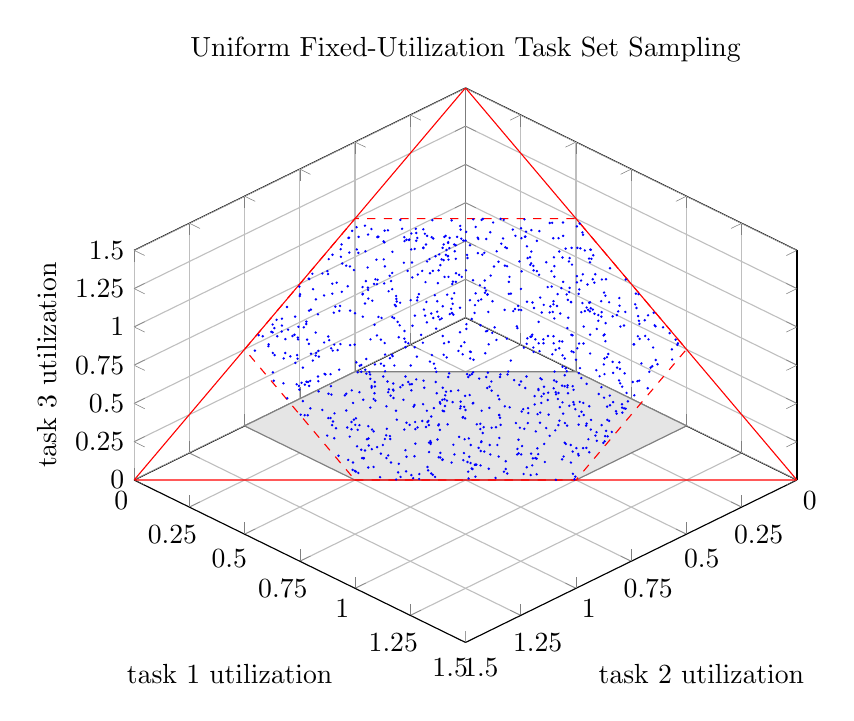
\begin{tikzpicture}
\begin{axis}[
    title={Uniform Fixed-Utilization Task Set Sampling},
    view={135}{45},
    xmin=0, xmax=1.5,
    ymin=0, ymax=1.5,
    zmin=0, zmax=1.5,
    xtick distance=0.25,
    ytick distance=0.25,
    ztick distance=0.25,
    xmajorgrids=true,
    ymajorgrids=true,
    zmajorgrids=true,
    xlabel=task 2 utilization,
    ylabel=task 1 utilization,
    zlabel=task 3 utilization
]
\addplot3[color=gray, fill=gray!20] coordinates 
{
    (1,0.5,0)
    (0.5,1,0)
    (0,1,0)
    (0,0.5,0)
    (0.5,0,0)
    (1,0,0)
    (1,0.5,0)
};
\addplot3[color=red] coordinates 
{
    (1.5,0,0)
    (0,1.5,0)
    (0,0,1.5)
    (1.5,0,0)
};
\addplot3[color=red, dashed] coordinates 
{
    (1,0.5,0)
    (0.5,1,0)
    (0,1,0.5)
    (0,0.5,1)
    (0.5,0,1)
    (1,0,0.5)
    (1,0.5,0)
};
\addplot3[only marks, color=blue, mark size=0.2pt] coordinates 
{
(0.688,0.445,0.367)(0.575,0.827,0.098)(0.081,0.714,0.705)(0.101,0.525,0.874)(0.79,0.479,0.231)(0.394,0.749,0.357)(0.949,0.185,0.366)(0.977,0.153,0.37)(0.409,0.246,0.845)(0.413,0.126,0.961)(0.757,0.6,0.143)(0.399,0.342,0.759)(0.576,0.175,0.749)(0.697,0.714,0.089)(0.944,0.358,0.198)(0.35,0.982,0.168)(0.887,0.382,0.231)(0.623,0.183,0.694)(0.231,0.626,0.643)(0.748,0.685,0.067)(0.937,0.326,0.237)(0.041,0.581,0.878)(0.978,0.352,0.17)(0.582,0.168,0.75)(0.885,0.548,0.067)(0.213,0.4,0.887)(0.696,0.745,0.059)(0.19,0.754,0.556)(0.372,0.343,0.785)(0.64,0.712,0.148)(0.107,0.441,0.952)(0.524,0.159,0.817)(0.323,0.654,0.523)(0.707,0.584,0.209)(0.693,0.441,0.366)(0.434,0.372,0.694)(0.865,0.449,0.186)(0.695,0.092,0.713)(0.209,0.607,0.684)(0.474,0.195,0.831)(0.701,0.509,0.29)(0.231,0.715,0.554)(0.479,0.148,0.873)(0.321,0.623,0.556)(0.404,0.181,0.915)(0.634,0.542,0.324)(0.366,0.863,0.271)(0.266,0.976,0.258)(0.329,0.623,0.548)(0.085,0.865,0.55)(0.177,0.873,0.45)(0.495,0.387,0.618)(0.728,0.562,0.21)(0.466,0.327,0.707)(0.389,0.166,0.945)(0.419,0.163,0.918)(0.771,0.322,0.407)(0.483,0.927,0.09)(0.603,0.305,0.592)(0.516,0.297,0.687)(0.412,0.552,0.536)(0.684,0.541,0.275)(0.655,0.407,0.438)(0.419,0.624,0.457)(0.12,0.624,0.756)(0.655,0.465,0.38)(0.101,0.715,0.684)(0.94,0.048,0.512)(0.558,0.666,0.276)(0.156,0.625,0.719)(0.446,0.639,0.415)(0.67,0.11,0.72)(0.867,0.176,0.457)(0.814,0.666,0.02)(0.566,0.168,0.766)(0.054,0.75,0.696)(0.527,0.394,0.579)(0.536,0.895,0.069)(0.378,0.259,0.863)(0.396,0.282,0.822)(0.171,0.649,0.68)(0.124,0.524,0.852)(0.741,0.413,0.346)(0.75,0.403,0.347)(0.844,0.135,0.521)(0.351,0.628,0.521)(0.072,0.921,0.507)(0.931,0.44,0.129)(0.081,0.664,0.755)(0.098,0.566,0.836)(0.669,0.446,0.385)(0.186,0.603,0.711)(0.553,0.709,0.238)(0.865,0.442,0.193)(0.584,0.818,0.098)(0.603,0.08,0.817)(0.435,0.274,0.791)(0.791,0.212,0.497)(0.396,0.178,0.926)(0.737,0.456,0.307)(0.281,0.357,0.862)(0.096,0.813,0.591)(0.494,0.595,0.411)(0.779,0.614,0.107)(0.393,0.349,0.758)(0.349,0.305,0.846)(0.052,0.615,0.833)(0.887,0.347,0.266)(0.605,0.041,0.854)(0.468,0.833,0.199)(0.702,0.695,0.103)(0.239,0.62,0.641)(0.062,0.454,0.984)(0.034,0.808,0.658)(0.519,0.487,0.494)(0.333,0.237,0.93)(0.116,0.954,0.43)(0.646,0.113,0.741)(0.779,0.307,0.414)(0.41,0.451,0.639)(0.147,0.676,0.677)(0.857,0.026,0.617)(0.078,0.705,0.717)(0.161,0.414,0.925)(0.73,0.04,0.73)(0.72,0.01,0.77)(0.42,0.488,0.592)(0.353,0.267,0.88)(0.346,0.445,0.709)(0.008,0.969,0.523)(0.185,0.575,0.74)(0.162,0.987,0.351)(0.446,0.69,0.364)(0.728,0.132,0.64)(0.738,0.559,0.203)(0.224,0.478,0.798)(0.618,0.359,0.523)(0.257,0.602,0.641)(0.416,0.876,0.208)(0.788,0.43,0.282)(0.285,0.222,0.993)(0.11,0.955,0.435)(0.242,0.383,0.875)(0.953,0.201,0.346)(0.17,0.396,0.934)(0.716,0.347,0.437)(0.943,0.079,0.478)(0.643,0.548,0.309)(0.676,0.073,0.751)(0.358,0.254,0.888)(0.509,0.354,0.637)(0.552,0.022,0.926)(0.604,0.443,0.453)(0.015,0.547,0.938)(0.967,0.231,0.302)(0.502,0.538,0.46)(0.472,0.809,0.219)(0.573,0.808,0.119)(0.437,0.813,0.25)(0.565,0.122,0.813)(0.433,0.408,0.659)(0.348,0.35,0.802)(0.304,0.545,0.651)(0.536,0.865,0.099)(0.942,0.474,0.084)(0.894,0.228,0.378)(0.998,0.252,0.25)(0.418,0.367,0.715)(0.99,0.262,0.248)(0.802,0.194,0.504)(0.415,0.962,0.123)(0.5,0.289,0.711)(0.365,0.629,0.506)(0.371,0.959,0.17)(0.904,0.031,0.565)(0.943,0.071,0.486)(0.527,0.755,0.218)(0.419,0.245,0.836)(0.891,0.597,0.012)(0.854,0.489,0.157)(0.409,0.314,0.777)(0.191,0.524,0.785)(0.86,0.102,0.538)(0.753,0.231,0.516)(0.417,0.163,0.92)(0.186,0.906,0.408)(0.282,0.26,0.958)(0.527,0.344,0.629)(0.336,0.671,0.493)(0.513,0.143,0.844)(0.424,0.849,0.227)(0.184,0.941,0.375)(0.321,0.33,0.849)(0.4,0.323,0.777)(0.424,0.147,0.929)(0.864,0.061,0.575)(0.172,0.95,0.378)(0.323,0.251,0.926)(0.59,0.588,0.322)(0.195,0.32,0.985)(0.121,0.737,0.642)(0.964,0.262,0.274)(0.423,0.955,0.122)(0.378,0.786,0.336)(0.189,0.724,0.587)(0.688,0.756,0.056)(0.342,0.859,0.299)(0.62,0.598,0.282)(0.358,0.893,0.249)(0.615,0.057,0.828)(0.565,0.724,0.211)(0.936,0.045,0.519)(0.84,0.123,0.537)(0.207,0.672,0.621)(0.123,0.421,0.956)(0.673,0.29,0.537)(0.291,0.311,0.898)(0.342,0.434,0.724)(0.688,0.346,0.466)(0.289,0.93,0.281)(0.866,0.083,0.551)(0.52,0.188,0.792)(0.58,0.019,0.901)(0.439,0.709,0.352)(0.525,0.587,0.388)(0.378,0.436,0.686)(0.912,0.209,0.379)(0.37,0.416,0.714)(0.498,0.816,0.186)(0.604,0.273,0.623)(0.921,0.466,0.113)(0.037,0.478,0.985)(0.853,0.242,0.405)(0.13,0.745,0.625)(0.846,0.182,0.472)(0.091,0.622,0.787)(0.191,0.857,0.452)(0.659,0.718,0.123)(0.286,0.71,0.504)(0.897,0.381,0.222)(0.424,0.276,0.8)(0.298,0.279,0.923)(0.297,0.705,0.498)(0.481,0.219,0.8)(0.222,0.756,0.522)(0.164,0.378,0.958)(0.259,0.562,0.679)(0.823,0.052,0.625)(0.259,0.51,0.731)(0.682,0.653,0.165)(0.635,0.624,0.241)(0.138,0.65,0.712)(0.931,0.204,0.365)(0.277,0.406,0.817)(0.047,0.567,0.886)(0.211,0.29,0.999)(0.483,0.086,0.931)(0.118,0.385,0.997)(0.379,0.28,0.841)(0.478,0.955,0.067)(0.382,0.274,0.844)(0.836,0.17,0.494)(0.351,0.788,0.361)(0.449,0.669,0.382)(0.696,0.266,0.538)(0.755,0.641,0.104)(0.816,0.647,0.037)(0.563,0.215,0.722)(0.895,0.449,0.156)(0.405,0.345,0.75)(0.257,0.966,0.277)(0.599,0.456,0.445)(0.559,0.263,0.678)(0.504,0.484,0.512)(0.033,0.967,0.5)(0.61,0.07,0.82)(0.611,0.381,0.508)(0.081,0.534,0.885)(0.903,0.479,0.118)(0.575,0.26,0.665)(0.839,0.572,0.089)(0.424,0.157,0.919)(0.243,0.289,0.968)(0.622,0.35,0.528)(0.149,0.42,0.931)(0.53,0.127,0.843)(0.659,0.543,0.298)(0.215,0.613,0.672)(0.26,0.318,0.922)(0.368,0.916,0.216)(0.825,0.253,0.422)(0.618,0.669,0.213)(0.853,0.643,0.004)(0.066,0.546,0.888)(0.311,0.535,0.654)(0.499,0.376,0.625)(0.892,0.13,0.478)(0.776,0.366,0.358)(0.895,0.275,0.33)(0.942,0.321,0.237)(0.63,0.572,0.298)(0.442,0.384,0.674)(0.39,0.254,0.856)(0.138,0.705,0.657)(0.979,0.494,0.027)(0.381,0.791,0.328)(0.71,0.655,0.135)(0.702,0.009,0.789)(0.595,0.562,0.343)(0.628,0.326,0.546)(0.408,0.762,0.33)(0.637,0.624,0.239)(0.37,0.196,0.934)(0.768,0.357,0.375)(0.164,0.442,0.894)(0.581,0.654,0.265)(0.625,0.601,0.274)(0.889,0.016,0.595)(0.007,0.931,0.562)(0.677,0.344,0.479)(0.898,0.138,0.464)(0.325,0.774,0.401)(0.293,0.817,0.39)(0.328,0.813,0.359)(0.934,0.016,0.55)(0.027,0.592,0.881)(0.042,0.612,0.846)(0.564,0.253,0.683)(0.706,0.551,0.243)(0.418,0.762,0.32)(0.619,0.686,0.195)(0.527,0.561,0.412)(0.357,0.845,0.298)(0.058,0.845,0.597)(0.533,0.562,0.405)(0.226,0.79,0.484)(0.887,0.529,0.084)(0.046,0.827,0.627)(0.461,0.4,0.639)(0.413,0.743,0.344)(0.933,0.517,0.05)(0.774,0.074,0.652)(0.688,0.416,0.396)(0.661,0.547,0.292)(0.863,0.618,0.019)(0.667,0.045,0.788)(0.788,0.3,0.412)(0.614,0.148,0.738)(0.052,0.987,0.461)(0.983,0.269,0.248)(0.089,0.486,0.925)(0.551,0.219,0.73)(0.174,0.637,0.689)(0.766,0.294,0.44)(0.573,0.372,0.555)(0.735,0.539,0.226)(0.792,0.515,0.193)(0.282,0.613,0.605)(0.414,0.69,0.396)(0.026,0.882,0.592)(0.468,0.397,0.635)(0.195,0.835,0.47)(0.157,0.697,0.646)(0.362,0.955,0.183)(0.585,0.62,0.295)(0.888,0.583,0.029)(0.376,0.333,0.791)(0.279,0.906,0.315)(0.289,0.688,0.523)(0.343,0.65,0.507)(0.433,0.746,0.321)(0.386,0.725,0.389)(0.726,0.676,0.098)(0.519,0.785,0.196)(0.339,0.426,0.735)(0.967,0.373,0.16)(0.276,0.252,0.972)(0.366,0.175,0.959)(0.527,0.773,0.2)(0.994,0.126,0.38)(0.461,0.406,0.633)(0.293,0.742,0.465)(0.815,0.66,0.025)(0.791,0.174,0.535)(0.258,0.407,0.835)(0.492,0.364,0.644)(0.164,0.462,0.874)(0.756,0.004,0.74)(0.402,0.211,0.887)(0.262,0.461,0.777)(0.601,0.294,0.605)(0.571,0.873,0.056)(0.527,0.043,0.93)(0.134,0.735,0.631)(0.865,0.628,0.007)(0.067,0.895,0.538)(0.527,0.852,0.121)(0.725,0.553,0.222)(0.185,0.466,0.849)(0.632,0.36,0.508)(0.855,0.315,0.33)(0.901,0.049,0.55)(0.515,0.662,0.323)(0.611,0.589,0.3)(0.775,0.46,0.265)(0.292,0.84,0.368)(0.911,0.141,0.448)(0.077,0.498,0.925)(0.519,0.672,0.309)(0.195,0.567,0.738)(0.166,0.6,0.734)(0.245,0.751,0.504)(0.351,0.919,0.23)(0.302,0.416,0.782)(0.342,0.803,0.355)(0.277,0.795,0.428)(0.082,0.773,0.645)(0.483,0.057,0.96)(0.244,0.836,0.42)(0.991,0.416,0.093)(0.664,0.081,0.755)(0.55,0.023,0.927)(0.758,0.541,0.201)(0.807,0.129,0.564)(0.396,0.77,0.334)(0.454,0.908,0.138)(0.935,0.193,0.372)(0.74,0.754,0.006)(0.7,0.742,0.058)(0.55,0.702,0.248)(0.701,0.456,0.343)(0.445,0.921,0.134)(0.755,0.596,0.149)(0.232,0.57,0.698)(0.138,0.412,0.95)(0.67,0.205,0.625)(0.558,0.473,0.469)(0.87,0.568,0.062)(0.786,0.165,0.549)(0.979,0.026,0.495)(0.092,0.777,0.631)(0.397,0.824,0.279)(0.721,0.766,0.013)(0.004,0.729,0.767)(0.638,0.82,0.042)(0.342,0.577,0.581)(0.304,0.266,0.93)(0.362,0.282,0.856)(0.531,0.188,0.781)(0.851,0.173,0.476)(0.389,0.21,0.901)(0.415,0.514,0.571)(0.538,0.201,0.761)(0.867,0.427,0.206)(0.337,0.953,0.21)(0.361,0.991,0.148)(0.026,0.593,0.881)(0.774,0.507,0.219)(0.216,0.842,0.442)(0.392,0.524,0.584)(0.551,0.848,0.101)(0.866,0.228,0.406)(0.836,0.321,0.343)(0.72,0.425,0.355)(0.206,0.97,0.324)(0.544,0.551,0.405)(0.52,0.698,0.282)(0.348,0.436,0.716)(0.1,0.652,0.748)(0.53,0.017,0.953)(0.678,0.814,0.008)(0.669,0.566,0.265)(0.917,0.382,0.201)(0.259,0.314,0.927)(0.347,0.469,0.684)(0.164,0.758,0.578)(0.824,0.092,0.584)(0.946,0.506,0.048)(0.91,0.117,0.473)(0.251,0.959,0.29)(0.727,0.492,0.281)(0.794,0.567,0.139)(0.373,0.843,0.284)(0.012,0.541,0.947)(0.743,0.294,0.463)(0.299,0.551,0.65)(0.011,0.905,0.584)(0.006,0.957,0.537)(0.373,0.919,0.208)(0.729,0.402,0.369)(0.83,0.474,0.196)(0.929,0.106,0.465)(0.273,0.358,0.869)(0.288,0.344,0.868)(0.692,0.328,0.48)(0.711,0.426,0.363)(0.105,0.544,0.851)(0.713,0.745,0.042)(0.647,0.821,0.032)(0.803,0.202,0.495)(0.453,0.643,0.404)(0.667,0.48,0.353)(0.373,0.794,0.333)(0.232,0.746,0.522)(0.903,0.465,0.132)(0.57,0.162,0.768)(0.378,0.972,0.15)(0.823,0.015,0.662)(0.89,0.283,0.327)(0.766,0.312,0.422)(0.361,0.215,0.924)(0.472,0.344,0.684)(0.555,0.241,0.704)(0.34,0.572,0.588)(0.276,0.674,0.55)(0.369,0.44,0.691)(0.503,0.859,0.138)(0.888,0.073,0.539)(0.436,0.687,0.377)(0.453,0.938,0.109)(0.643,0.832,0.025)(0.679,0.031,0.79)(0.03,0.798,0.672)(0.743,0.066,0.691)(0.501,0.06,0.939)(0.022,0.848,0.63)(0.312,0.962,0.226)(0.52,0.638,0.342)(0.298,0.536,0.666)(0.15,0.592,0.758)(0.56,0.461,0.479)(0.829,0.557,0.114)(0.388,0.9,0.212)(0.692,0.433,0.375)(0.026,0.886,0.588)(0.649,0.519,0.332)(0.939,0.478,0.083)(0.603,0.161,0.736)(0.371,0.187,0.942)(0.292,0.292,0.916)(0.681,0.181,0.638)(0.517,0.626,0.357)(0.266,0.704,0.53)(0.687,0.165,0.648)(0.557,0.813,0.13)(0.53,0.282,0.688)(0.684,0.603,0.213)(0.013,0.517,0.97)(0.386,0.573,0.541)(0.215,0.915,0.37)(0.167,0.691,0.642)(0.616,0.616,0.268)(0.602,0.279,0.619)(0.62,0.018,0.862)(0.432,0.186,0.882)(0.632,0.36,0.508)(0.607,0.166,0.727)(0.5,0.782,0.218)(0.835,0.079,0.586)(0.64,0.556,0.304)(0.712,0.141,0.647)(0.362,0.209,0.929)(0.09,0.561,0.849)(0.215,0.395,0.89)(0.913,0.248,0.339)(0.844,0.485,0.171)(0.337,0.288,0.875)(0.66,0.729,0.111)(0.266,0.576,0.658)(0.868,0.599,0.033)(0.217,0.926,0.357)(0.394,0.437,0.669)(0.14,0.542,0.818)(0.997,0.19,0.313)(0.356,0.768,0.376)(0.278,0.959,0.263)(0.459,0.463,0.578)(0.195,0.503,0.802)(0.416,0.866,0.218)(0.352,0.816,0.332)(0.628,0.738,0.134)(0.402,0.844,0.254)(0.003,0.786,0.711)(0.618,0.196,0.686)(0.764,0.659,0.077)(0.717,0.707,0.076)(0.192,0.878,0.43)(0.678,0.348,0.474)(0.857,0.348,0.295)(0.584,0.391,0.525)(0.613,0.607,0.28)(0.456,0.09,0.954)(0.371,0.885,0.244)(0.578,0.9,0.022)(0.837,0.495,0.168)(0.359,0.76,0.381)(0.178,0.47,0.852)(0.328,0.178,0.994)(0.292,0.731,0.477)(0.27,0.77,0.46)(0.41,0.288,0.802)(0.234,0.269,0.997)(0.219,0.948,0.333)(0.203,0.373,0.924)(0.238,0.592,0.67)(0.58,0.718,0.202)(0.128,0.692,0.68)(0.411,0.783,0.306)(0.579,0.819,0.102)(0.509,0.292,0.699)(0.713,0.124,0.663)(0.671,0.695,0.134)(0.803,0.387,0.31)(0.828,0.365,0.307)(0.452,0.79,0.258)(0.76,0.602,0.138)(0.265,0.88,0.355)(0.812,0.091,0.597)(0.325,0.274,0.901)(0.21,0.454,0.836)(0.455,0.213,0.832)(0.448,0.252,0.8)(0.494,0.515,0.491)(0.938,0.478,0.084)(0.79,0.378,0.332)(0.357,0.882,0.261)(0.067,0.79,0.643)(0.892,0.027,0.581)(0.56,0.247,0.693)(0.761,0.596,0.143)(0.085,0.735,0.68)(0.45,0.454,0.596)(0.671,0.305,0.524)(0.761,0.326,0.413)(0.63,0.25,0.62)(0.161,0.786,0.553)(0.475,0.631,0.394)(0.526,0.423,0.551)(0.489,0.484,0.527)(0.861,0.315,0.324)(0.385,0.73,0.385)(0.465,0.249,0.786)(0.343,0.27,0.887)(0.094,0.963,0.443)(0.267,0.935,0.298)(0.146,0.709,0.645)(0.128,0.643,0.729)(0.762,0.659,0.079)(0.642,0.713,0.145)(0.192,0.485,0.823)(0.262,0.915,0.323)(0.305,0.657,0.538)(0.919,0.206,0.375)(0.947,0.343,0.21)(0.345,0.445,0.71)(0.078,0.654,0.768)(0.513,0.367,0.62)(0.704,0.583,0.213)(0.525,0.623,0.352)(0.479,0.108,0.913)(0.78,0.072,0.648)(0.288,0.661,0.551)(0.87,0.039,0.591)(0.349,0.25,0.901)(0.524,0.448,0.528)(0.906,0.592,0.002)(0.37,0.353,0.777)(0.773,0.023,0.704)(0.329,0.889,0.282)(0.728,0.74,0.032)(0.609,0.676,0.215)(0.764,0.332,0.404)(0.495,0.992,0.013)(0.394,0.95,0.156)(0.274,0.277,0.949)(0.865,0.231,0.404)(0.575,0.335,0.59)(0.411,0.741,0.348)(0.448,0.097,0.955)(0.555,0.063,0.882)(0.431,0.774,0.295)(0.296,0.492,0.712)(0.719,0.336,0.445)(0.613,0.547,0.34)(0.537,0.44,0.523)(0.166,0.624,0.71)(0.361,0.282,0.857)(0.106,0.807,0.587)(0.454,0.903,0.143)(0.449,0.762,0.289)(0.558,0.073,0.869)(0.503,0.62,0.377)(0.129,0.925,0.446)(0.659,0.247,0.594)(0.436,0.311,0.753)(0.756,0.43,0.314)(0.663,0.678,0.159)(0.001,0.518,0.981)(0.491,0.036,0.973)(0.233,0.712,0.555)(0.698,0.743,0.059)(0.827,0.396,0.277)(0.09,0.951,0.459)(0.807,0.087,0.606)(0.593,0.888,0.019)(0.625,0.522,0.353)(0.906,0.027,0.567)(0.217,0.379,0.904)(0.386,0.804,0.31)(0.048,0.684,0.768)(0.167,0.953,0.38)(0.367,0.991,0.142)(0.724,0.36,0.416)(0.109,0.872,0.519)(0.788,0.194,0.518)(0.314,0.956,0.23)(0.82,0.589,0.091)(0.211,0.879,0.41)(0.711,0.72,0.069)(0.482,0.088,0.93)(0.068,0.765,0.667)(0.423,0.193,0.884)(0.339,0.619,0.542)(0.382,0.821,0.297)(0.323,0.279,0.898)(0.592,0.514,0.394)(0.742,0.416,0.342)(0.22,0.332,0.948)(0.938,0.338,0.224)(0.131,0.691,0.678)(0.188,0.887,0.425)(0.501,0.385,0.614)(0.232,0.967,0.301)(0.313,0.771,0.416)(0.742,0.24,0.518)(0.649,0.544,0.307)(0.156,0.545,0.799)(0.053,0.838,0.609)(0.212,0.907,0.381)(0.351,0.385,0.764)(0.469,0.366,0.665)(0.229,0.69,0.581)(0.493,0.517,0.49)(0.166,0.339,0.995)(0.548,0.87,0.082)(0.417,0.977,0.106)(0.108,0.612,0.78)(0.345,0.41,0.745)(0.919,0.326,0.255)(0.334,0.256,0.91)(0.248,0.855,0.397)(0.712,0.596,0.192)(0.587,0.62,0.293)(0.857,0.098,0.545)(0.226,0.61,0.664)(0.401,0.156,0.943)(0.903,0.167,0.43)(0.607,0.87,0.023)(0.706,0.729,0.065)(0.047,0.606,0.847)(0.485,0.086,0.929)(0.858,0.159,0.483)(0.556,0.861,0.083)(0.48,0.764,0.256)(0.591,0.709,0.2)(0.187,0.484,0.829)(0.633,0.631,0.236)(0.127,0.959,0.414)(0.16,0.562,0.778)(0.435,0.855,0.21)(0.722,0.491,0.287)(0.766,0.539,0.195)(0.506,0.6,0.394)(0.28,0.934,0.286)(0.635,0.241,0.624)(0.186,0.832,0.482)(0.516,0.503,0.481)(0.674,0.67,0.156)(0.771,0.292,0.437)(0.886,0.218,0.396)(0.146,0.694,0.66)(0.462,0.281,0.757)(0.484,0.745,0.271)(0.479,0.112,0.909)(0.719,0.012,0.769)(0.701,0.133,0.666)(0.319,0.535,0.646)(0.171,0.33,0.999)(0.645,0.757,0.098)(0.242,0.336,0.922)(0.341,0.744,0.415)(0.983,0.482,0.035)(0.004,0.856,0.64)(0.811,0.639,0.05)(0.316,0.323,0.861)(0.772,0.341,0.387)(0.24,0.642,0.618)(0.336,0.513,0.651)(0.772,0.278,0.45)(0.928,0.456,0.116)(0.289,0.802,0.409)(0.738,0.385,0.377)(0.769,0.02,0.711)(0.878,0.528,0.094)(0.714,0.742,0.044)(0.273,0.469,0.758)(0.382,0.157,0.961)(0.55,0.866,0.084)(0.813,0.675,0.012)(0.086,0.874,0.54)(0.736,0.609,0.155)(0.842,0.501,0.157)(0.336,0.257,0.907)(0.822,0.342,0.336)(0.578,0.597,0.325)(0.55,0.321,0.629)(0.98,0.108,0.412)(0.757,0.407,0.336)(0.911,0.395,0.194)(0.463,0.552,0.485)(0.445,0.955,0.1)(0.667,0.57,0.263)(0.929,0.405,0.166)(0.608,0.69,0.202)(0.217,0.646,0.637)(0.068,0.449,0.983)(0.605,0.468,0.427)(0.058,0.675,0.767)(0.48,0.455,0.565)(0.986,0.475,0.039)(0.327,0.989,0.184)(0.625,0.537,0.338)(0.157,0.786,0.557)(0.63,0.78,0.09)(0.802,0.394,0.304)(0.428,0.456,0.616)(0.325,0.412,0.763)(0.734,0.324,0.442)(0.452,0.858,0.19)(0.396,0.416,0.688)(0.326,0.625,0.549)(0.64,0.185,0.675)(0.575,0.255,0.67)(0.203,0.832,0.465)(0.323,0.639,0.538)(0.216,0.289,0.995)(0.401,0.21,0.889)(0.938,0.551,0.011)(0.018,0.672,0.81)(0.498,0.321,0.681)(0.653,0.738,0.109)(0.663,0.038,0.799)(0.351,0.659,0.49)(0.345,0.988,0.167)(0.008,0.779,0.713)(0.495,0.981,0.024)(0.941,0.005,0.554)(0.338,0.8,0.362)(0.971,0.462,0.067)(0.297,0.287,0.916)(0.107,0.63,0.763)(0.705,0.53,0.265)(0.333,0.822,0.345)(0.419,0.512,0.569)(0.536,0.361,0.603)(0.284,0.887,0.329)(0.062,0.504,0.934)(0.375,0.774,0.351)(0.438,0.94,0.122)(0.591,0.026,0.883)(0.89,0.451,0.159)(0.328,0.238,0.934)(0.511,0.711,0.278)(0.753,0.525,0.222)(0.54,0.559,0.401)(0.455,0.39,0.655)(0.87,0.496,0.134)(0.587,0.435,0.478)(0.807,0.167,0.526)(0.171,0.648,0.681)(0.843,0.634,0.023)(0.151,0.516,0.833)(0.447,0.959,0.094)(0.626,0.161,0.713)(0.539,0.086,0.875)(0.27,0.548,0.682)(0.618,0.341,0.541)(0.875,0.266,0.359)(0.272,0.697,0.531)(0.885,0.405,0.21)(0.313,0.706,0.481)(0.721,0.553,0.226)(0.11,0.871,0.519)(0.15,0.419,0.931)(0.922,0.202,0.376)(0.924,0.216,0.36)(0.692,0.37,0.438)(0.887,0.487,0.126)(0.251,0.976,0.273)(0.21,0.624,0.666)(0.609,0.477,0.414)(0.628,0.162,0.71)(0.338,0.974,0.188)(0.549,0.702,0.249)(0.947,0.193,0.36)(0.145,0.746,0.609)(0.637,0.018,0.845)(0.518,0.33,0.652)(0.676,0.781,0.043)(0.558,0.19,0.752)(0.147,0.618,0.735)(0.595,0.144,0.761)(0.502,0.995,0.003)(0.483,0.242,0.775)(0.94,0.292,0.268)(0.133,0.767,0.6)(0.251,0.429,0.82)(0.783,0.358,0.359)(0.717,0.077,0.706)(0.039,0.85,0.611)(0.314,0.753,0.433)(0.36,0.851,0.289)(0.553,0.793,0.154)(0.977,0.446,0.077)(0.031,0.609,0.86)(0.063,0.65,0.787)(0.894,0.395,0.211)(0.189,0.512,0.799)(0.438,0.543,0.519)(0.758,0.419,0.323)(0.611,0.755,0.134)(0.367,0.29,0.843)(0.143,0.394,0.963)(0.982,0.486,0.032)(0.233,0.862,0.405)(0.131,0.454,0.915)(0.891,0.508,0.101)(0.475,0.856,0.169)(0.364,0.275,0.861)(0.63,0.495,0.375)(0.136,0.712,0.652)(0.738,0.366,0.396)(0.507,0.528,0.465)(0.764,0.65,0.086)(0.786,0.361,0.353)(0.583,0.509,0.408)(0.437,0.354,0.709)(0.674,0.273,0.553)(0.097,0.579,0.824)(0.578,0.052,0.87)(0.31,0.763,0.427)(0.187,0.494,0.819)(0.859,0.085,0.556)(0.767,0.099,0.634)(0.513,0.02,0.967)(0.771,0.518,0.211)(0.247,0.435,0.818)(0.845,0.169,0.486)(0.254,0.972,0.274)(0.104,0.77,0.626)(0.461,0.787,0.252)(0.408,0.529,0.563)(0.312,0.665,0.523)(0.898,0.41,0.192)(0.471,0.754,0.275)(0.915,0.099,0.486)(0.492,0.746,0.262)(0.469,0.627,0.404)(0.431,0.155,0.914)(0.871,0.016,0.613)(0.168,0.801,0.531)(0.545,0.954,0.001)(0.492,0.929,0.079)(0.88,0.384,0.236)(0.882,0.05,0.568)(0.547,0.559,0.394)(0.14,0.724,0.636)(0.147,0.702,0.651)(0.281,0.965,0.254)(0.053,0.559,0.888)(0.012,0.971,0.517)(0.601,0.096,0.803)(0.37,0.937,0.193)(0.4,0.105,0.995)(0.624,0.404,0.472)(0.593,0.746,0.161)(0.603,0.327,0.57)(0.767,0.646,0.087)(0.336,0.869,0.295)(0.587,0.864,0.049)(0.773,0.207,0.52)(0.264,0.744,0.492)(0.291,0.496,0.713)(0.346,0.795,0.359)(0.623,0.805,0.072)(0.068,0.881,0.551)(0.621,0.699,0.18)(0.377,0.48,0.643)(0.655,0.562,0.283)(0.261,0.75,0.489)
};
\end{axis}
\end{tikzpicture}
\caption{1000 random task sets consisting of three tasks with a total utilization of 1.5 generated by the Stick-Breaking Approach with a precision value of 1000. The 1.5 scaled unit simplex and its intersection with the unit cube are shown.}
\label{fig_stickbreak}
\end{figure}
\subsection{Task Set Generation}
To compare various scheduling algorithms, we must generate task sets to serve as our medium on which comparisons can be made. This can be done by generating $n$ uniformly random tasks with a fixed utilization sum of $u$, where the utilization of a task is denoted as its execution time divided by its period.

\subsubsection{Continuous Simplex Sampling} If we define the utilization of task $i$ as $x_i$ in the $n$-dimensional coordinate point $p = [x_1, x_2, \ldots, x_n] \in \mathbf{R}^n$, this problem can be reduced to sampling a random point on the simplex $S_{n,u}$ defined by the corner points $[u,0,\ldots,0], [0,u,\ldots,0], \ldots, [0,0,\ldots,u]$, which is equivalent to the $n$-dimensional unit simplex scaled by a factor of $u$. An approach for simplex sampling specifically for task-set generation is the UUniFast-Discard algorithm \cite{uunifast} with an improved multi-core variant defined by Stafford's RandFixedSum algorithm \cite{randfixedsum}, which both require uniform sampling on real numbers. This problem is also solved by the Dirichlet process, a method for sampling from a unit simplex \cite{dirichlet}.

\subsubsection{Discrete Simplex Sampling} If we constrain the possible utilizations to a set of uniformly spaced discrete values, we can use the Stick-Breaking Approach to sample points on discrete points within a Dirichlet distribution by picking $n-1$ partition points on the closed interval $[1,u)$ to partition into $n$ sub-intervals, then assigning $x_i$ to the size of the $i$th sub-interval \cite{dirichlet}. The advantage of discretized sampling is it replaces uniform sampling on real numbers with uniform sampling on integer values. This is advantageous for computers since they operate on finite-precision values. The pseudo-code used for generating MARISA's fixed-utilization random task sets using the stick-breaking algorithm is shown in algorithm \ref{rtset_alg}.

\subsubsection{Bounding Task Utilizations} The Stick-Breaking Approach and UUniFast-Discard both share a problem when creating task sets with utilizations greater than one for the multi-core case, as the sample space is modeled as the intersection of an $n$-dimensional unit cube and the simplex described above. This is because individual task utilizations must be limited to at most one. This can be circumvented by discarding invalid task sets, thus allowing simplex sampling to extend to multi-core. However, this issue increases when the target utilization approaches the number of tasks, as there are fewer ways to partition utilization in a way that guarantees each task gets at most a utilization of one. This correlates to a smaller intersection between the simplex and the unit cube. RandFixedSum addresses this issue by breaking the intersection into a set of simplexes and sampling from each proportionally \cite{randfixedsum}. Implementation of RandFixedSum is outside the scope of MARISA currently. A visualization of the intersection described, sampled by MARISA's implementation of the Stick Breaking Approach with three tasks and a precision of 1000, is shown in figure \ref{fig_stickbreak}.

\subsection{Comparison Procedure}
For this experiment, we will check the schedulability, context switches, and job-level migrations of each algorithm at certain utilization values on random task sets generated as defined above. Similar to the schedulability test used in a paper outlining EDZL schedulability analysis \cite{edzl}, we will compare with core counts of 2, 4, and 8. For a task set to be feasible, the size of the task set must be greater than the core count, since otherwise the average utilization per task must exceed $1$, which produces invalid tasks. In addition, the closer the core count is to the task count, the larger the issue motivating Stafford's RandFixedSum becomes, which is described in section 4.2.3. Therefore, the number of tasks will be fixed at 12 to ensure sufficient feasible task sets for $8$ cores. Periods for tasks will be uniformly sampled between $4$ and $16$. The reasoning behind choosing these period values is covered in section 4.3.1. Utilization steps of $0.005k$ will be used up to utilization $k$, with $50$ trials per utilization, where $k$ is the number of processors. This amounts to $10^4$ trials per experiment. Since PD$^2$ is only optimal on discrete time, we will use a quantum of length $0.1$ and round execution times up. This will keep PD$^2$ comparable in terms of schedulability without overly inflating context switches and migration times. The utilization of these schedules will be based on the original task set utilization, as we consider the rounding-up process to be contained in the PD$^2$ scheduler rather than the task set generation.

\subsection{Schedulability Percentage vs Utilization}
Schedulability will be checked by simulating up to time $2H$ where $H = \text{LCM}\{\tau_i\}$ for tasks $\tau_i$ in the task set \cite{leung}. Our period choice of $4$ to $16$ guarantees that $H \leq 27720$ which is the lcm of all period choices. The resulting graphs for each core count used are shown in figure \ref{fig_sched}.

\subsection{Comparison of Context Switches}
We define a context switch as an event where a core switches the job running on it or when a core switches between running and idle. For data collection, using the same task sets generated for schedulability tests, we will also check for the number of context switches up to time $1000$ for each trial. Since for some utilization values, some generated task sets are not schedulable on certain algorithms, we will only count context switches on schedulable task sets. The compared value is the mean number of context switches per schedulable task set at each utilization. The resulting graphs for each core count used are shown in figure \ref{fig_cswitch}.

\subsection{Job-Level Migrations}
We define a job-level migration as an event where a job that was last executed on one core is scheduled onto a different core. Fresh jobs that have not been previously executed cannot migrate. From this definition, it is clear that migrations must occur during context switches. As such, we should expect the migrations to roughly scale with the number of context switches. Like context switch comparison, we will check the number of migrations up to time $1000$ on the same task sets used for schedulability, counting only schedulable task sets. The compared value is the mean number of migrations per schedulable task set at each utilization. The resulting graphs for each core count used are shown in figure \ref{fig_mig}.

\subsection{Experiment Conclusion}
\subsubsection{Schedulability} The schedulability of GEDF appears to perform worse as the core count increases and is by far the worst-performing algorithm. Due to the rounding-up procedure, PD$^2$ appears to fall off at roughly $0.1$ utilization regardless of core count. EDZL appears near optimal, with its fall-off point scaling linearly with the core count. And lastly, LLREF and U-EDF are constant lines at the top due to being optimal on continuous time.

\subsubsection{Context Switches} GEDF and EDZL behave almost identically due to EDZL using primarily GEDF. The number of context switches with PD$^2$ scales almost perfectly linearly, with very little deviation. This is likely due to separating each task into subtasks with execution times equivalent to the quantum size. With $y_i$ denoting the context switch count of task $i$ and $C_i, T_i, U_i$ denoting the execution time, period, and utilization of task $i$ respectively, this means $y_i \approx \frac{C_i}{q}$ and so $\frac{y_i}{T_i} = \frac{C_i}{qT_i} = qU_i$ where $q = 0.1$ denotes the quantum length. Thus the total context switch count $y = \frac{tU}{q} = 10^4U$ where $U$ is the task set utilization and $t = 1000$ is the simulated time. This equation matches the resulting data and explains the consistency of the line. This also implies the effects of early releasing on the context switch count are not very significant, as this is not accounted for in the above equation. U-EDF behaves strangely, likely due to its way of partitioning onto cores. It only schedules onto enough cores to satisfy the task-set utilization, which explains the constant context-switch count at $\leq1$ utilization, as it is simply doing uniprocessor EDF. The jumps might be better explained by the migrations. As the authors of U-EDF suggested \cite{uedf}, it has generally lower context switches than the other optimal schedulers, scaling linearly over time and without the spike at the end that LLREF has.

\subsubsection{Job-Level Migrations} The proportion of context switches that are job-level migrations appears to behave roughly the same regardless of the scheduling algorithm, as in at near zero utilization, roughly 5\% of context switches, with the proportion increasing exponentially near full utilization. This tailing exponential scaling for EDF and EDZL is more distinguishable with 8 cores. For U-EDF, since it only uses enough cores to satisfy the task-set utilization, the migrations start at zero for task sets schedulable by uniprocessor and spike at each subsequent whole utilization as a core reaches full capacity, before overflowing to the next core. The original paper covering U-EDF \cite{uedf} does not do this specific type of utilization vs migration comparison, so it is not conclusive if this is a flawed implementation issue or inherent to the algorithm. However, this is likely due to U-EDF only scheduling to minimal cores, which causes high contention over the available cores just below whole utilization values. U-EDF has comparable migration counts to PD$^2$.

\begin{figure}
\scalebox{.95}{
\input{2core_sched}
}\hspace{1px}
\scalebox{.95}{
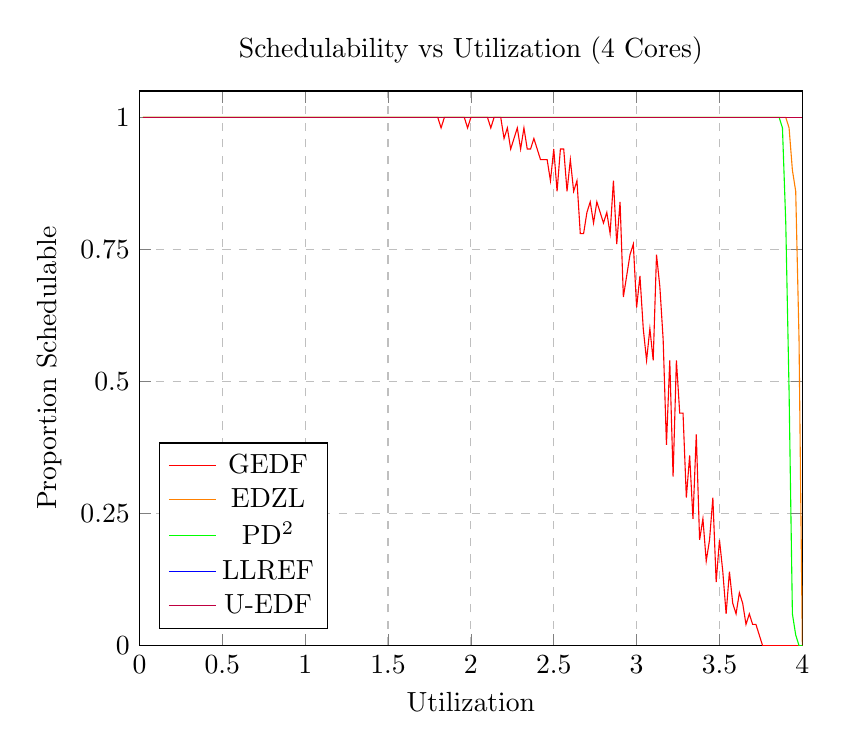
\begin{tikzpicture}
\begin{axis}[
    title={Schedulability vs Utilization (4 Cores)},
    xlabel={Utilization},
    ylabel={Proportion Schedulable},
    xmin=0, xmax=4,
    ymin=0, ymax=1.05,
    xtick distance=0.5,
    ytick distance=0.25,
    xmajorgrids=true,
    ymajorgrids=true,
    grid style=dashed,
    legend pos=south west,
]
\legend{GEDF, EDZL, PD$^2$, LLREF, U-EDF}
\addplot[color=red]
coordinates {
(0.02,1)(0.04,1)(0.06,1)(0.08,1)(0.1,1)(0.12,1)(0.14,1)(0.16,1)(0.18,1)(0.2,1)(0.22,1)(0.24,1)(0.26,1)(0.28,1)(0.3,1)(0.32,1)(0.34,1)(0.36,1)(0.38,1)(0.4,1)(0.42,1)(0.44,1)(0.46,1)(0.48,1)(0.5,1)(0.52,1)(0.54,1)(0.56,1)(0.58,1)(0.6,1)(0.62,1)(0.64,1)(0.66,1)(0.68,1)(0.7,1)(0.72,1)(0.74,1)(0.76,1)(0.78,1)(0.8,1)(0.82,1)(0.84,1)(0.86,1)(0.88,1)(0.9,1)(0.92,1)(0.94,1)(0.96,1)(0.98,1)(1,1)(1.02,1)(1.04,1)(1.06,1)(1.08,1)(1.1,1)(1.12,1)(1.14,1)(1.16,1)(1.18,1)(1.2,1)(1.22,1)(1.24,1)(1.26,1)(1.28,1)(1.3,1)(1.32,1)(1.34,1)(1.36,1)(1.38,1)(1.4,1)(1.42,1)(1.44,1)(1.46,1)(1.48,1)(1.5,1)(1.52,1)(1.54,1)(1.56,1)(1.58,1)(1.6,1)(1.62,1)(1.64,1)(1.66,1)(1.68,1)(1.7,1)(1.72,1)(1.74,1)(1.76,1)(1.78,1)(1.8,1)(1.82,0.98)(1.84,1)(1.86,1)(1.88,1)(1.9,1)(1.92,1)(1.94,1)(1.96,1)(1.98,0.98)(2,1)(2.02,1)(2.04,1)(2.06,1)(2.08,1)(2.1,1)(2.12,0.98)(2.14,1)(2.16,1)(2.18,1)(2.2,0.96)(2.22,0.98)(2.24,0.94)(2.26,0.96)(2.28,0.98)(2.3,0.94)(2.32,0.98)(2.34,0.94)(2.36,0.94)(2.38,0.96)(2.4,0.94)(2.42,0.92)(2.44,0.92)(2.46,0.92)(2.48,0.88)(2.5,0.94)(2.52,0.86)(2.54,0.94)(2.56,0.94)(2.58,0.86)(2.6,0.92)(2.62,0.86)(2.64,0.88)(2.66,0.78)(2.68,0.78)(2.7,0.82)(2.72,0.84)(2.74,0.8)(2.76,0.84)(2.78,0.82)(2.8,0.8)(2.82,0.82)(2.84,0.78)(2.86,0.88)(2.88,0.76)(2.9,0.84)(2.92,0.66)(2.94,0.7)(2.96,0.74)(2.98,0.76)(3,0.64)(3.02,0.7)(3.04,0.6)(3.06,0.54)(3.08,0.6)(3.1,0.54)(3.12,0.74)(3.14,0.68)(3.16,0.58)(3.18,0.38)(3.2,0.54)(3.22,0.32)(3.24,0.54)(3.26,0.44)(3.28,0.44)(3.3,0.28)(3.32,0.36)(3.34,0.24)(3.36,0.4)(3.38,0.2)(3.4,0.24)(3.42,0.16)(3.44,0.2)(3.46,0.28)(3.48,0.12)(3.5,0.2)(3.52,0.14)(3.54,0.06)(3.56,0.14)(3.58,0.08)(3.6,0.06)(3.62,0.1)(3.64,0.08)(3.66,0.04)(3.68,0.06)(3.7,0.04)(3.72,0.04)(3.74,0.02)(3.76,0)(3.78,0)(3.8,0)(3.82,0)(3.84,0)(3.86,0)(3.88,0)(3.9,0)(3.92,0)(3.94,0)(3.96,0)(3.98,0)(4,0)
};
\addplot[color=orange]
coordinates {
(0.02,1)(0.04,1)(0.06,1)(0.08,1)(0.1,1)(0.12,1)(0.14,1)(0.16,1)(0.18,1)(0.2,1)(0.22,1)(0.24,1)(0.26,1)(0.28,1)(0.3,1)(0.32,1)(0.34,1)(0.36,1)(0.38,1)(0.4,1)(0.42,1)(0.44,1)(0.46,1)(0.48,1)(0.5,1)(0.52,1)(0.54,1)(0.56,1)(0.58,1)(0.6,1)(0.62,1)(0.64,1)(0.66,1)(0.68,1)(0.7,1)(0.72,1)(0.74,1)(0.76,1)(0.78,1)(0.8,1)(0.82,1)(0.84,1)(0.86,1)(0.88,1)(0.9,1)(0.92,1)(0.94,1)(0.96,1)(0.98,1)(1,1)(1.02,1)(1.04,1)(1.06,1)(1.08,1)(1.1,1)(1.12,1)(1.14,1)(1.16,1)(1.18,1)(1.2,1)(1.22,1)(1.24,1)(1.26,1)(1.28,1)(1.3,1)(1.32,1)(1.34,1)(1.36,1)(1.38,1)(1.4,1)(1.42,1)(1.44,1)(1.46,1)(1.48,1)(1.5,1)(1.52,1)(1.54,1)(1.56,1)(1.58,1)(1.6,1)(1.62,1)(1.64,1)(1.66,1)(1.68,1)(1.7,1)(1.72,1)(1.74,1)(1.76,1)(1.78,1)(1.8,1)(1.82,1)(1.84,1)(1.86,1)(1.88,1)(1.9,1)(1.92,1)(1.94,1)(1.96,1)(1.98,1)(2,1)(2.02,1)(2.04,1)(2.06,1)(2.08,1)(2.1,1)(2.12,1)(2.14,1)(2.16,1)(2.18,1)(2.2,1)(2.22,1)(2.24,1)(2.26,1)(2.28,1)(2.3,1)(2.32,1)(2.34,1)(2.36,1)(2.38,1)(2.4,1)(2.42,1)(2.44,1)(2.46,1)(2.48,1)(2.5,1)(2.52,1)(2.54,1)(2.56,1)(2.58,1)(2.6,1)(2.62,1)(2.64,1)(2.66,1)(2.68,1)(2.7,1)(2.72,1)(2.74,1)(2.76,1)(2.78,1)(2.8,1)(2.82,1)(2.84,1)(2.86,1)(2.88,1)(2.9,1)(2.92,1)(2.94,1)(2.96,1)(2.98,1)(3,1)(3.02,1)(3.04,1)(3.06,1)(3.08,1)(3.1,1)(3.12,1)(3.14,1)(3.16,1)(3.18,1)(3.2,1)(3.22,1)(3.24,1)(3.26,1)(3.28,1)(3.3,1)(3.32,1)(3.34,1)(3.36,1)(3.38,1)(3.4,1)(3.42,1)(3.44,1)(3.46,1)(3.48,1)(3.5,1)(3.52,1)(3.54,1)(3.56,1)(3.58,1)(3.6,1)(3.62,1)(3.64,1)(3.66,1)(3.68,1)(3.7,1)(3.72,1)(3.74,1)(3.76,1)(3.78,1)(3.8,1)(3.82,1)(3.84,1)(3.86,1)(3.88,1)(3.9,1)(3.92,0.98)(3.94,0.9)(3.96,0.86)(3.98,0.58)(4,0)
};
\addplot[color=green]
coordinates {
(0.02,1)(0.04,1)(0.06,1)(0.08,1)(0.1,1)(0.12,1)(0.14,1)(0.16,1)(0.18,1)(0.2,1)(0.22,1)(0.24,1)(0.26,1)(0.28,1)(0.3,1)(0.32,1)(0.34,1)(0.36,1)(0.38,1)(0.4,1)(0.42,1)(0.44,1)(0.46,1)(0.48,1)(0.5,1)(0.52,1)(0.54,1)(0.56,1)(0.58,1)(0.6,1)(0.62,1)(0.64,1)(0.66,1)(0.68,1)(0.7,1)(0.72,1)(0.74,1)(0.76,1)(0.78,1)(0.8,1)(0.82,1)(0.84,1)(0.86,1)(0.88,1)(0.9,1)(0.92,1)(0.94,1)(0.96,1)(0.98,1)(1,1)(1.02,1)(1.04,1)(1.06,1)(1.08,1)(1.1,1)(1.12,1)(1.14,1)(1.16,1)(1.18,1)(1.2,1)(1.22,1)(1.24,1)(1.26,1)(1.28,1)(1.3,1)(1.32,1)(1.34,1)(1.36,1)(1.38,1)(1.4,1)(1.42,1)(1.44,1)(1.46,1)(1.48,1)(1.5,1)(1.52,1)(1.54,1)(1.56,1)(1.58,1)(1.6,1)(1.62,1)(1.64,1)(1.66,1)(1.68,1)(1.7,1)(1.72,1)(1.74,1)(1.76,1)(1.78,1)(1.8,1)(1.82,1)(1.84,1)(1.86,1)(1.88,1)(1.9,1)(1.92,1)(1.94,1)(1.96,1)(1.98,1)(2,1)(2.02,1)(2.04,1)(2.06,1)(2.08,1)(2.1,1)(2.12,1)(2.14,1)(2.16,1)(2.18,1)(2.2,1)(2.22,1)(2.24,1)(2.26,1)(2.28,1)(2.3,1)(2.32,1)(2.34,1)(2.36,1)(2.38,1)(2.4,1)(2.42,1)(2.44,1)(2.46,1)(2.48,1)(2.5,1)(2.52,1)(2.54,1)(2.56,1)(2.58,1)(2.6,1)(2.62,1)(2.64,1)(2.66,1)(2.68,1)(2.7,1)(2.72,1)(2.74,1)(2.76,1)(2.78,1)(2.8,1)(2.82,1)(2.84,1)(2.86,1)(2.88,1)(2.9,1)(2.92,1)(2.94,1)(2.96,1)(2.98,1)(3,1)(3.02,1)(3.04,1)(3.06,1)(3.08,1)(3.1,1)(3.12,1)(3.14,1)(3.16,1)(3.18,1)(3.2,1)(3.22,1)(3.24,1)(3.26,1)(3.28,1)(3.3,1)(3.32,1)(3.34,1)(3.36,1)(3.38,1)(3.4,1)(3.42,1)(3.44,1)(3.46,1)(3.48,1)(3.5,1)(3.52,1)(3.54,1)(3.56,1)(3.58,1)(3.6,1)(3.62,1)(3.64,1)(3.66,1)(3.68,1)(3.7,1)(3.72,1)(3.74,1)(3.76,1)(3.78,1)(3.8,1)(3.82,1)(3.84,1)(3.86,1)(3.88,0.98)(3.9,0.8)(3.92,0.48)(3.94,0.06)(3.96,0.02)(3.98,0)(4,0)
};
\addplot[color=blue]
coordinates {
(0.02,1)(0.04,1)(0.06,1)(0.08,1)(0.1,1)(0.12,1)(0.14,1)(0.16,1)(0.18,1)(0.2,1)(0.22,1)(0.24,1)(0.26,1)(0.28,1)(0.3,1)(0.32,1)(0.34,1)(0.36,1)(0.38,1)(0.4,1)(0.42,1)(0.44,1)(0.46,1)(0.48,1)(0.5,1)(0.52,1)(0.54,1)(0.56,1)(0.58,1)(0.6,1)(0.62,1)(0.64,1)(0.66,1)(0.68,1)(0.7,1)(0.72,1)(0.74,1)(0.76,1)(0.78,1)(0.8,1)(0.82,1)(0.84,1)(0.86,1)(0.88,1)(0.9,1)(0.92,1)(0.94,1)(0.96,1)(0.98,1)(1,1)(1.02,1)(1.04,1)(1.06,1)(1.08,1)(1.1,1)(1.12,1)(1.14,1)(1.16,1)(1.18,1)(1.2,1)(1.22,1)(1.24,1)(1.26,1)(1.28,1)(1.3,1)(1.32,1)(1.34,1)(1.36,1)(1.38,1)(1.4,1)(1.42,1)(1.44,1)(1.46,1)(1.48,1)(1.5,1)(1.52,1)(1.54,1)(1.56,1)(1.58,1)(1.6,1)(1.62,1)(1.64,1)(1.66,1)(1.68,1)(1.7,1)(1.72,1)(1.74,1)(1.76,1)(1.78,1)(1.8,1)(1.82,1)(1.84,1)(1.86,1)(1.88,1)(1.9,1)(1.92,1)(1.94,1)(1.96,1)(1.98,1)(2,1)(2.02,1)(2.04,1)(2.06,1)(2.08,1)(2.1,1)(2.12,1)(2.14,1)(2.16,1)(2.18,1)(2.2,1)(2.22,1)(2.24,1)(2.26,1)(2.28,1)(2.3,1)(2.32,1)(2.34,1)(2.36,1)(2.38,1)(2.4,1)(2.42,1)(2.44,1)(2.46,1)(2.48,1)(2.5,1)(2.52,1)(2.54,1)(2.56,1)(2.58,1)(2.6,1)(2.62,1)(2.64,1)(2.66,1)(2.68,1)(2.7,1)(2.72,1)(2.74,1)(2.76,1)(2.78,1)(2.8,1)(2.82,1)(2.84,1)(2.86,1)(2.88,1)(2.9,1)(2.92,1)(2.94,1)(2.96,1)(2.98,1)(3,1)(3.02,1)(3.04,1)(3.06,1)(3.08,1)(3.1,1)(3.12,1)(3.14,1)(3.16,1)(3.18,1)(3.2,1)(3.22,1)(3.24,1)(3.26,1)(3.28,1)(3.3,1)(3.32,1)(3.34,1)(3.36,1)(3.38,1)(3.4,1)(3.42,1)(3.44,1)(3.46,1)(3.48,1)(3.5,1)(3.52,1)(3.54,1)(3.56,1)(3.58,1)(3.6,1)(3.62,1)(3.64,1)(3.66,1)(3.68,1)(3.7,1)(3.72,1)(3.74,1)(3.76,1)(3.78,1)(3.8,1)(3.82,1)(3.84,1)(3.86,1)(3.88,1)(3.9,1)(3.92,1)(3.94,1)(3.96,1)(3.98,1)(4,1)
};
\addplot[color=purple]
coordinates {
(0.02,1)(0.04,1)(0.06,1)(0.08,1)(0.1,1)(0.12,1)(0.14,1)(0.16,1)(0.18,1)(0.2,1)(0.22,1)(0.24,1)(0.26,1)(0.28,1)(0.3,1)(0.32,1)(0.34,1)(0.36,1)(0.38,1)(0.4,1)(0.42,1)(0.44,1)(0.46,1)(0.48,1)(0.5,1)(0.52,1)(0.54,1)(0.56,1)(0.58,1)(0.6,1)(0.62,1)(0.64,1)(0.66,1)(0.68,1)(0.7,1)(0.72,1)(0.74,1)(0.76,1)(0.78,1)(0.8,1)(0.82,1)(0.84,1)(0.86,1)(0.88,1)(0.9,1)(0.92,1)(0.94,1)(0.96,1)(0.98,1)(1,1)(1.02,1)(1.04,1)(1.06,1)(1.08,1)(1.1,1)(1.12,1)(1.14,1)(1.16,1)(1.18,1)(1.2,1)(1.22,1)(1.24,1)(1.26,1)(1.28,1)(1.3,1)(1.32,1)(1.34,1)(1.36,1)(1.38,1)(1.4,1)(1.42,1)(1.44,1)(1.46,1)(1.48,1)(1.5,1)(1.52,1)(1.54,1)(1.56,1)(1.58,1)(1.6,1)(1.62,1)(1.64,1)(1.66,1)(1.68,1)(1.7,1)(1.72,1)(1.74,1)(1.76,1)(1.78,1)(1.8,1)(1.82,1)(1.84,1)(1.86,1)(1.88,1)(1.9,1)(1.92,1)(1.94,1)(1.96,1)(1.98,1)(2,1)(2.02,1)(2.04,1)(2.06,1)(2.08,1)(2.1,1)(2.12,1)(2.14,1)(2.16,1)(2.18,1)(2.2,1)(2.22,1)(2.24,1)(2.26,1)(2.28,1)(2.3,1)(2.32,1)(2.34,1)(2.36,1)(2.38,1)(2.4,1)(2.42,1)(2.44,1)(2.46,1)(2.48,1)(2.5,1)(2.52,1)(2.54,1)(2.56,1)(2.58,1)(2.6,1)(2.62,1)(2.64,1)(2.66,1)(2.68,1)(2.7,1)(2.72,1)(2.74,1)(2.76,1)(2.78,1)(2.8,1)(2.82,1)(2.84,1)(2.86,1)(2.88,1)(2.9,1)(2.92,1)(2.94,1)(2.96,1)(2.98,1)(3,1)(3.02,1)(3.04,1)(3.06,1)(3.08,1)(3.1,1)(3.12,1)(3.14,1)(3.16,1)(3.18,1)(3.2,1)(3.22,1)(3.24,1)(3.26,1)(3.28,1)(3.3,1)(3.32,1)(3.34,1)(3.36,1)(3.38,1)(3.4,1)(3.42,1)(3.44,1)(3.46,1)(3.48,1)(3.5,1)(3.52,1)(3.54,1)(3.56,1)(3.58,1)(3.6,1)(3.62,1)(3.64,1)(3.66,1)(3.68,1)(3.7,1)(3.72,1)(3.74,1)(3.76,1)(3.78,1)(3.8,1)(3.82,1)(3.84,1)(3.86,1)(3.88,1)(3.9,1)(3.92,1)(3.94,1)(3.96,1)(3.98,1)(4,1)
};
\end{axis}
\end{tikzpicture}
}\hspace{1px}
\scalebox{.95}{
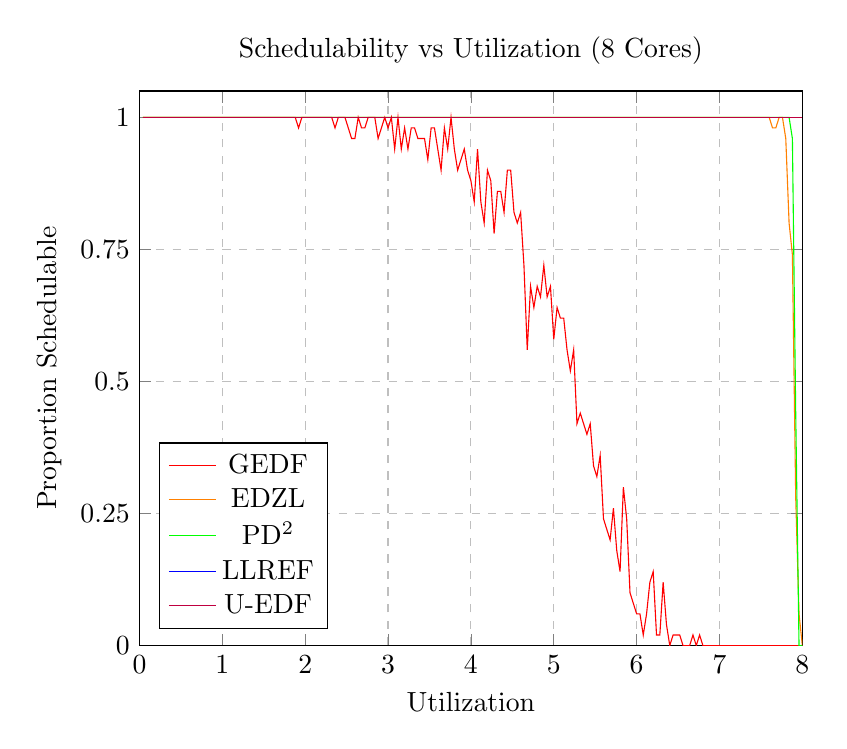
\begin{tikzpicture}
\begin{axis}[
    title={Schedulability vs Utilization (8 Cores)},
    xlabel={Utilization},
    ylabel={Proportion Schedulable},
    xmin=0, xmax=8,
    ymin=0, ymax=1.05,
    xtick distance=1,
    ytick distance=0.25,
    xmajorgrids=true,
    ymajorgrids=true,
    grid style=dashed,
    legend pos=south west,
]
\legend{GEDF, EDZL, PD$^2$, LLREF, U-EDF}
\addplot[color=red]
coordinates {
(0.04,1)(0.08,1)(0.12,1)(0.16,1)(0.2,1)(0.24,1)(0.28,1)(0.32,1)(0.36,1)(0.4,1)(0.44,1)(0.48,1)(0.52,1)(0.56,1)(0.6,1)(0.64,1)(0.68,1)(0.72,1)(0.76,1)(0.8,1)(0.84,1)(0.88,1)(0.92,1)(0.96,1)(1,1)(1.04,1)(1.08,1)(1.12,1)(1.16,1)(1.2,1)(1.24,1)(1.28,1)(1.32,1)(1.36,1)(1.4,1)(1.44,1)(1.48,1)(1.52,1)(1.56,1)(1.6,1)(1.64,1)(1.68,1)(1.72,1)(1.76,1)(1.8,1)(1.84,1)(1.88,1)(1.92,0.98)(1.96,1)(2,1)(2.04,1)(2.08,1)(2.12,1)(2.16,1)(2.2,1)(2.24,1)(2.28,1)(2.32,1)(2.36,0.98)(2.4,1)(2.44,1)(2.48,1)(2.52,0.98)(2.56,0.96)(2.6,0.96)(2.64,1)(2.68,0.98)(2.72,0.98)(2.76,1)(2.8,1)(2.84,1)(2.88,0.96)(2.92,0.98)(2.96,1)(3,0.98)(3.04,1)(3.08,0.94)(3.12,1)(3.16,0.94)(3.2,0.98)(3.24,0.94)(3.28,0.98)(3.32,0.98)(3.36,0.96)(3.4,0.96)(3.44,0.96)(3.48,0.92)(3.52,0.98)(3.56,0.98)(3.6,0.94)(3.64,0.9)(3.68,0.98)(3.72,0.94)(3.76,1)(3.8,0.94)(3.84,0.9)(3.88,0.92)(3.92,0.94)(3.96,0.9)(4,0.88)(4.04,0.84)(4.08,0.94)(4.12,0.84)(4.16,0.8)(4.2,0.9)(4.24,0.88)(4.28,0.78)(4.32,0.86)(4.36,0.86)(4.4,0.82)(4.44,0.9)(4.48,0.9)(4.52,0.82)(4.56,0.8)(4.6,0.82)(4.64,0.72)(4.68,0.56)(4.72,0.68)(4.76,0.64)(4.8,0.68)(4.84,0.66)(4.88,0.72)(4.92,0.66)(4.96,0.68)(5,0.58)(5.04,0.64)(5.08,0.62)(5.12,0.62)(5.16,0.56)(5.2,0.52)(5.24,0.56)(5.28,0.42)(5.32,0.44)(5.36,0.42)(5.4,0.4)(5.44,0.42)(5.48,0.34)(5.52,0.32)(5.56,0.36)(5.6,0.24)(5.64,0.22)(5.68,0.2)(5.72,0.26)(5.76,0.18)(5.8,0.14)(5.84,0.3)(5.88,0.24)(5.92,0.1)(5.96,0.08)(6,0.06)(6.04,0.06)(6.08,0.02)(6.12,0.06)(6.16,0.12)(6.2,0.14)(6.24,0.02)(6.28,0.02)(6.32,0.12)(6.36,0.04)(6.4,0)(6.44,0.02)(6.48,0.02)(6.52,0.02)(6.56,0)(6.6,0)(6.64,0)(6.68,0.02)(6.72,0)(6.76,0.02)(6.8,0)(6.84,0)(6.88,0)(6.92,0)(6.96,0)(7,0)(7.04,0)(7.08,0)(7.12,0)(7.16,0)(7.2,0)(7.24,0)(7.28,0)(7.32,0)(7.36,0)(7.4,0)(7.44,0)(7.48,0)(7.52,0)(7.56,0)(7.6,0)(7.64,0)(7.68,0)(7.72,0)(7.76,0)(7.8,0)(7.84,0)(7.88,0)(7.92,0)(7.96,0)(8,0)
};
\addplot[color=orange]
coordinates {
(0.04,1)(0.08,1)(0.12,1)(0.16,1)(0.2,1)(0.24,1)(0.28,1)(0.32,1)(0.36,1)(0.4,1)(0.44,1)(0.48,1)(0.52,1)(0.56,1)(0.6,1)(0.64,1)(0.68,1)(0.72,1)(0.76,1)(0.8,1)(0.84,1)(0.88,1)(0.92,1)(0.96,1)(1,1)(1.04,1)(1.08,1)(1.12,1)(1.16,1)(1.2,1)(1.24,1)(1.28,1)(1.32,1)(1.36,1)(1.4,1)(1.44,1)(1.48,1)(1.52,1)(1.56,1)(1.6,1)(1.64,1)(1.68,1)(1.72,1)(1.76,1)(1.8,1)(1.84,1)(1.88,1)(1.92,1)(1.96,1)(2,1)(2.04,1)(2.08,1)(2.12,1)(2.16,1)(2.2,1)(2.24,1)(2.28,1)(2.32,1)(2.36,1)(2.4,1)(2.44,1)(2.48,1)(2.52,1)(2.56,1)(2.6,1)(2.64,1)(2.68,1)(2.72,1)(2.76,1)(2.8,1)(2.84,1)(2.88,1)(2.92,1)(2.96,1)(3,1)(3.04,1)(3.08,1)(3.12,1)(3.16,1)(3.2,1)(3.24,1)(3.28,1)(3.32,1)(3.36,1)(3.4,1)(3.44,1)(3.48,1)(3.52,1)(3.56,1)(3.6,1)(3.64,1)(3.68,1)(3.72,1)(3.76,1)(3.8,1)(3.84,1)(3.88,1)(3.92,1)(3.96,1)(4,1)(4.04,1)(4.08,1)(4.12,1)(4.16,1)(4.2,1)(4.24,1)(4.28,1)(4.32,1)(4.36,1)(4.4,1)(4.44,1)(4.48,1)(4.52,1)(4.56,1)(4.6,1)(4.64,1)(4.68,1)(4.72,1)(4.76,1)(4.8,1)(4.84,1)(4.88,1)(4.92,1)(4.96,1)(5,1)(5.04,1)(5.08,1)(5.12,1)(5.16,1)(5.2,1)(5.24,1)(5.28,1)(5.32,1)(5.36,1)(5.4,1)(5.44,1)(5.48,1)(5.52,1)(5.56,1)(5.6,1)(5.64,1)(5.68,1)(5.72,1)(5.76,1)(5.8,1)(5.84,1)(5.88,1)(5.92,1)(5.96,1)(6,1)(6.04,1)(6.08,1)(6.12,1)(6.16,1)(6.2,1)(6.24,1)(6.28,1)(6.32,1)(6.36,1)(6.4,1)(6.44,1)(6.48,1)(6.52,1)(6.56,1)(6.6,1)(6.64,1)(6.68,1)(6.72,1)(6.76,1)(6.8,1)(6.84,1)(6.88,1)(6.92,1)(6.96,1)(7,1)(7.04,1)(7.08,1)(7.12,1)(7.16,1)(7.2,1)(7.24,1)(7.28,1)(7.32,1)(7.36,1)(7.4,1)(7.44,1)(7.48,1)(7.52,1)(7.56,1)(7.6,1)(7.64,0.98)(7.68,0.98)(7.72,1)(7.76,1)(7.8,0.96)(7.84,0.8)(7.88,0.74)(7.92,0.28)(7.96,0.06)(8,0)
};
\addplot[color=green]
coordinates {
(0.04,1)(0.08,1)(0.12,1)(0.16,1)(0.2,1)(0.24,1)(0.28,1)(0.32,1)(0.36,1)(0.4,1)(0.44,1)(0.48,1)(0.52,1)(0.56,1)(0.6,1)(0.64,1)(0.68,1)(0.72,1)(0.76,1)(0.8,1)(0.84,1)(0.88,1)(0.92,1)(0.96,1)(1,1)(1.04,1)(1.08,1)(1.12,1)(1.16,1)(1.2,1)(1.24,1)(1.28,1)(1.32,1)(1.36,1)(1.4,1)(1.44,1)(1.48,1)(1.52,1)(1.56,1)(1.6,1)(1.64,1)(1.68,1)(1.72,1)(1.76,1)(1.8,1)(1.84,1)(1.88,1)(1.92,1)(1.96,1)(2,1)(2.04,1)(2.08,1)(2.12,1)(2.16,1)(2.2,1)(2.24,1)(2.28,1)(2.32,1)(2.36,1)(2.4,1)(2.44,1)(2.48,1)(2.52,1)(2.56,1)(2.6,1)(2.64,1)(2.68,1)(2.72,1)(2.76,1)(2.8,1)(2.84,1)(2.88,1)(2.92,1)(2.96,1)(3,1)(3.04,1)(3.08,1)(3.12,1)(3.16,1)(3.2,1)(3.24,1)(3.28,1)(3.32,1)(3.36,1)(3.4,1)(3.44,1)(3.48,1)(3.52,1)(3.56,1)(3.6,1)(3.64,1)(3.68,1)(3.72,1)(3.76,1)(3.8,1)(3.84,1)(3.88,1)(3.92,1)(3.96,1)(4,1)(4.04,1)(4.08,1)(4.12,1)(4.16,1)(4.2,1)(4.24,1)(4.28,1)(4.32,1)(4.36,1)(4.4,1)(4.44,1)(4.48,1)(4.52,1)(4.56,1)(4.6,1)(4.64,1)(4.68,1)(4.72,1)(4.76,1)(4.8,1)(4.84,1)(4.88,1)(4.92,1)(4.96,1)(5,1)(5.04,1)(5.08,1)(5.12,1)(5.16,1)(5.2,1)(5.24,1)(5.28,1)(5.32,1)(5.36,1)(5.4,1)(5.44,1)(5.48,1)(5.52,1)(5.56,1)(5.6,1)(5.64,1)(5.68,1)(5.72,1)(5.76,1)(5.8,1)(5.84,1)(5.88,1)(5.92,1)(5.96,1)(6,1)(6.04,1)(6.08,1)(6.12,1)(6.16,1)(6.2,1)(6.24,1)(6.28,1)(6.32,1)(6.36,1)(6.4,1)(6.44,1)(6.48,1)(6.52,1)(6.56,1)(6.6,1)(6.64,1)(6.68,1)(6.72,1)(6.76,1)(6.8,1)(6.84,1)(6.88,1)(6.92,1)(6.96,1)(7,1)(7.04,1)(7.08,1)(7.12,1)(7.16,1)(7.2,1)(7.24,1)(7.28,1)(7.32,1)(7.36,1)(7.4,1)(7.44,1)(7.48,1)(7.52,1)(7.56,1)(7.6,1)(7.64,1)(7.68,1)(7.72,1)(7.76,1)(7.8,1)(7.84,1)(7.88,0.96)(7.92,0.44)(7.96,0)(8,0)
};
\addplot[color=blue]
coordinates {
(0.04,1)(0.08,1)(0.12,1)(0.16,1)(0.2,1)(0.24,1)(0.28,1)(0.32,1)(0.36,1)(0.4,1)(0.44,1)(0.48,1)(0.52,1)(0.56,1)(0.6,1)(0.64,1)(0.68,1)(0.72,1)(0.76,1)(0.8,1)(0.84,1)(0.88,1)(0.92,1)(0.96,1)(1,1)(1.04,1)(1.08,1)(1.12,1)(1.16,1)(1.2,1)(1.24,1)(1.28,1)(1.32,1)(1.36,1)(1.4,1)(1.44,1)(1.48,1)(1.52,1)(1.56,1)(1.6,1)(1.64,1)(1.68,1)(1.72,1)(1.76,1)(1.8,1)(1.84,1)(1.88,1)(1.92,1)(1.96,1)(2,1)(2.04,1)(2.08,1)(2.12,1)(2.16,1)(2.2,1)(2.24,1)(2.28,1)(2.32,1)(2.36,1)(2.4,1)(2.44,1)(2.48,1)(2.52,1)(2.56,1)(2.6,1)(2.64,1)(2.68,1)(2.72,1)(2.76,1)(2.8,1)(2.84,1)(2.88,1)(2.92,1)(2.96,1)(3,1)(3.04,1)(3.08,1)(3.12,1)(3.16,1)(3.2,1)(3.24,1)(3.28,1)(3.32,1)(3.36,1)(3.4,1)(3.44,1)(3.48,1)(3.52,1)(3.56,1)(3.6,1)(3.64,1)(3.68,1)(3.72,1)(3.76,1)(3.8,1)(3.84,1)(3.88,1)(3.92,1)(3.96,1)(4,1)(4.04,1)(4.08,1)(4.12,1)(4.16,1)(4.2,1)(4.24,1)(4.28,1)(4.32,1)(4.36,1)(4.4,1)(4.44,1)(4.48,1)(4.52,1)(4.56,1)(4.6,1)(4.64,1)(4.68,1)(4.72,1)(4.76,1)(4.8,1)(4.84,1)(4.88,1)(4.92,1)(4.96,1)(5,1)(5.04,1)(5.08,1)(5.12,1)(5.16,1)(5.2,1)(5.24,1)(5.28,1)(5.32,1)(5.36,1)(5.4,1)(5.44,1)(5.48,1)(5.52,1)(5.56,1)(5.6,1)(5.64,1)(5.68,1)(5.72,1)(5.76,1)(5.8,1)(5.84,1)(5.88,1)(5.92,1)(5.96,1)(6,1)(6.04,1)(6.08,1)(6.12,1)(6.16,1)(6.2,1)(6.24,1)(6.28,1)(6.32,1)(6.36,1)(6.4,1)(6.44,1)(6.48,1)(6.52,1)(6.56,1)(6.6,1)(6.64,1)(6.68,1)(6.72,1)(6.76,1)(6.8,1)(6.84,1)(6.88,1)(6.92,1)(6.96,1)(7,1)(7.04,1)(7.08,1)(7.12,1)(7.16,1)(7.2,1)(7.24,1)(7.28,1)(7.32,1)(7.36,1)(7.4,1)(7.44,1)(7.48,1)(7.52,1)(7.56,1)(7.6,1)(7.64,1)(7.68,1)(7.72,1)(7.76,1)(7.8,1)(7.84,1)(7.88,1)(7.92,1)(7.96,1)(8,1)
};
\addplot[color=purple]
coordinates {
(0.04,1)(0.08,1)(0.12,1)(0.16,1)(0.2,1)(0.24,1)(0.28,1)(0.32,1)(0.36,1)(0.4,1)(0.44,1)(0.48,1)(0.52,1)(0.56,1)(0.6,1)(0.64,1)(0.68,1)(0.72,1)(0.76,1)(0.8,1)(0.84,1)(0.88,1)(0.92,1)(0.96,1)(1,1)(1.04,1)(1.08,1)(1.12,1)(1.16,1)(1.2,1)(1.24,1)(1.28,1)(1.32,1)(1.36,1)(1.4,1)(1.44,1)(1.48,1)(1.52,1)(1.56,1)(1.6,1)(1.64,1)(1.68,1)(1.72,1)(1.76,1)(1.8,1)(1.84,1)(1.88,1)(1.92,1)(1.96,1)(2,1)(2.04,1)(2.08,1)(2.12,1)(2.16,1)(2.2,1)(2.24,1)(2.28,1)(2.32,1)(2.36,1)(2.4,1)(2.44,1)(2.48,1)(2.52,1)(2.56,1)(2.6,1)(2.64,1)(2.68,1)(2.72,1)(2.76,1)(2.8,1)(2.84,1)(2.88,1)(2.92,1)(2.96,1)(3,1)(3.04,1)(3.08,1)(3.12,1)(3.16,1)(3.2,1)(3.24,1)(3.28,1)(3.32,1)(3.36,1)(3.4,1)(3.44,1)(3.48,1)(3.52,1)(3.56,1)(3.6,1)(3.64,1)(3.68,1)(3.72,1)(3.76,1)(3.8,1)(3.84,1)(3.88,1)(3.92,1)(3.96,1)(4,1)(4.04,1)(4.08,1)(4.12,1)(4.16,1)(4.2,1)(4.24,1)(4.28,1)(4.32,1)(4.36,1)(4.4,1)(4.44,1)(4.48,1)(4.52,1)(4.56,1)(4.6,1)(4.64,1)(4.68,1)(4.72,1)(4.76,1)(4.8,1)(4.84,1)(4.88,1)(4.92,1)(4.96,1)(5,1)(5.04,1)(5.08,1)(5.12,1)(5.16,1)(5.2,1)(5.24,1)(5.28,1)(5.32,1)(5.36,1)(5.4,1)(5.44,1)(5.48,1)(5.52,1)(5.56,1)(5.6,1)(5.64,1)(5.68,1)(5.72,1)(5.76,1)(5.8,1)(5.84,1)(5.88,1)(5.92,1)(5.96,1)(6,1)(6.04,1)(6.08,1)(6.12,1)(6.16,1)(6.2,1)(6.24,1)(6.28,1)(6.32,1)(6.36,1)(6.4,1)(6.44,1)(6.48,1)(6.52,1)(6.56,1)(6.6,1)(6.64,1)(6.68,1)(6.72,1)(6.76,1)(6.8,1)(6.84,1)(6.88,1)(6.92,1)(6.96,1)(7,1)(7.04,1)(7.08,1)(7.12,1)(7.16,1)(7.2,1)(7.24,1)(7.28,1)(7.32,1)(7.36,1)(7.4,1)(7.44,1)(7.48,1)(7.52,1)(7.56,1)(7.6,1)(7.64,1)(7.68,1)(7.72,1)(7.76,1)(7.8,1)(7.84,1)(7.88,1)(7.92,1)(7.96,1)(8,1)
};
\end{axis}
\end{tikzpicture}
}
\caption{Schedulability experimental results.}
\label{fig_sched}
\end{figure}

\begin{figure}
\scalebox{.95}{
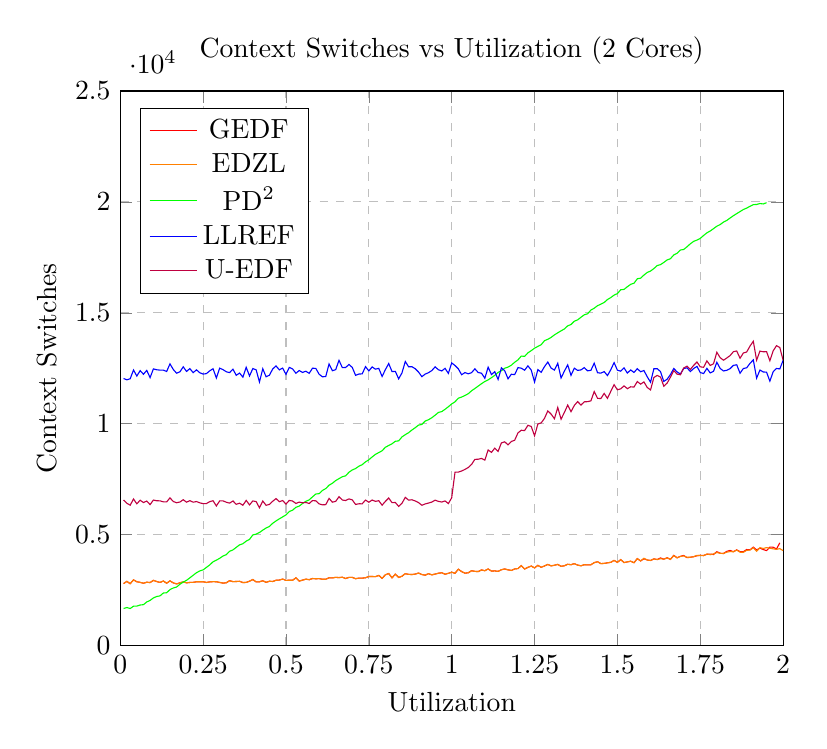
\begin{tikzpicture}
\begin{axis}[
    title={Context Switches vs Utilization (2 Cores)},
    xlabel={Utilization},
    ylabel={Context Switches},
    xmin=0, xmax=2,
    ymin=0, ymax=25000,
    xtick distance=0.25,
    ytick distance=5000,
    xmajorgrids=true,
    ymajorgrids=true,
    grid style=dashed,
    legend pos=north west,
]
\legend{GEDF, EDZL, PD$^2$, LLREF, U-EDF}
\addplot[color=red]
coordinates {
(0.01,2793)(0.02,2892.72)(0.03,2787.46)(0.04,2960.66)(0.05,2876.3)(0.06,2847.72)(0.07,2810.62)(0.08,2854.82)(0.09,2838.36)(0.1,2939.76)(0.11,2884.46)(0.12,2846.2)(0.13,2908.7)(0.14,2810.14)(0.15,2915.52)(0.16,2824.48)(0.17,2778.92)(0.18,2829.3)(0.19,2869.04)(0.2,2828.52)(0.21,2844.62)(0.22,2848.98)(0.23,2875.28)(0.24,2875.94)(0.25,2876.18)(0.26,2844.36)(0.27,2869.96)(0.28,2880.42)(0.29,2876.84)(0.3,2845.84)(0.31,2814.54)(0.32,2830.6)(0.33,2924.08)(0.34,2881.54)(0.35,2887.72)(0.36,2896.6)(0.37,2838.72)(0.38,2846.76)(0.39,2903.18)(0.4,2975.56)(0.41,2869.26)(0.42,2873.92)(0.43,2919.76)(0.44,2851.36)(0.45,2900.06)(0.46,2888.28)(0.47,2942.54)(0.48,2953.6)(0.49,2997.32)(0.5,2937.28)(0.51,2945.96)(0.52,2943.56)(0.53,3052.34)(0.54,2905.98)(0.55,2949.68)(0.56,2993.34)(0.57,2969)(0.58,3022.14)(0.59,3010.2)(0.6,3017.84)(0.61,2988.98)(0.62,2990.26)(0.63,3054.22)(0.64,3050.44)(0.65,3074.06)(0.66,3063.64)(0.67,3079.74)(0.68,3020.98)(0.69,3073.62)(0.7,3072.8)(0.71,3013.62)(0.72,3038.86)(0.73,3040)(0.74,3055.18)(0.75,3114.14)(0.76,3113.04)(0.77,3105.9)(0.78,3162.66)(0.79,3030.1)(0.8,3191.46)(0.81,3247.32)(0.82,3053.38)(0.83,3218.48)(0.84,3072.3)(0.85,3124.88)(0.86,3240.48)(0.87,3209.04)(0.88,3201.74)(0.89,3222.26)(0.9,3267.28)(0.91,3202.38)(0.92,3171.64)(0.93,3240.82)(0.94,3186.9)(0.95,3223.46)(0.96,3260.4)(0.97,3280.54)(0.98,3216.78)(0.99,3257.24)(1,3306.26)(1.01,3259.02)(1.02,3440.08)(1.03,3334)(1.04,3262.34)(1.05,3280.38)(1.06,3373.4)(1.07,3343.14)(1.08,3334.7)(1.09,3409.98)(1.1,3373.18)(1.11,3453.46)(1.12,3354.68)(1.13,3366.2)(1.14,3343.34)(1.15,3418.94)(1.16,3452.38)(1.17,3413.6)(1.18,3386.5)(1.19,3452.72)(1.2,3471.72)(1.21,3600.18)(1.22,3452.14)(1.23,3525.32)(1.24,3582.78)(1.25,3500.6)(1.26,3613.1)(1.27,3528.96)(1.28,3587.8)(1.29,3657.44)(1.3,3593.12)(1.31,3619.12)(1.32,3659.64)(1.33,3571.18)(1.34,3597.98)(1.35,3663.82)(1.36,3644.92)(1.37,3691.54)(1.38,3626.84)(1.39,3596.14)(1.4,3643.94)(1.41,3634.22)(1.42,3641.14)(1.43,3737.3)(1.44,3778.98)(1.45,3693.64)(1.46,3703.28)(1.47,3729.24)(1.48,3751.98)(1.49,3838.06)(1.5,3749.7)(1.51,3873.52)(1.52,3740.8)(1.53,3770.53)(1.54,3801.76)(1.55,3734.32)(1.56,3918.3)(1.57,3813.45)(1.58,3912.55)(1.59,3856.73)(1.6,3835.58)(1.61,3908.62)(1.62,3875.59)(1.63,3951.02)(1.64,3893.72)(1.65,3957.2)(1.66,3885.4)(1.67,4067.15)(1.68,3958.6)(1.69,4020.66)(1.7,4059.62)(1.71,3961.56)(1.72,3980.62)(1.73,4006.04)(1.74,4046.38)(1.75,4069.15)(1.76,4060.52)(1.77,4112.31)(1.78,4122.2)(1.79,4104.22)(1.8,4231.22)(1.81,4160.21)(1.82,4149.4)(1.83,4247.3)(1.84,4286.41)(1.85,4230.81)(1.86,4313.56)(1.87,4232.4)(1.88,4230.4)(1.89,4328.74)(1.9,4314.6)(1.91,4436.4)(1.92,4310.7)(1.93,4390.52)(1.94,4327.6)(1.95,4281.08)(1.96,4437.69)(1.97,4433)(1.98,4350.3)(1.99,4631.25)
};
\addplot[color=orange]
coordinates {
(0.01,2793)(0.02,2892.72)(0.03,2787.46)(0.04,2960.66)(0.05,2876.3)(0.06,2847.72)(0.07,2810.62)(0.08,2854.82)(0.09,2838.36)(0.1,2939.76)(0.11,2884.46)(0.12,2846.2)(0.13,2908.7)(0.14,2810.14)(0.15,2915.52)(0.16,2824.48)(0.17,2778.92)(0.18,2829.3)(0.19,2869.04)(0.2,2828.52)(0.21,2844.62)(0.22,2848.98)(0.23,2875.28)(0.24,2875.94)(0.25,2876.18)(0.26,2844.36)(0.27,2869.96)(0.28,2880.42)(0.29,2876.84)(0.3,2845.84)(0.31,2814.54)(0.32,2830.6)(0.33,2924.08)(0.34,2881.54)(0.35,2887.72)(0.36,2896.6)(0.37,2838.72)(0.38,2846.76)(0.39,2903.18)(0.4,2975.56)(0.41,2869.26)(0.42,2873.92)(0.43,2919.76)(0.44,2851.36)(0.45,2900.06)(0.46,2888.28)(0.47,2942.54)(0.48,2953.6)(0.49,2997.32)(0.5,2937.28)(0.51,2945.96)(0.52,2943.56)(0.53,3052.34)(0.54,2905.98)(0.55,2949.68)(0.56,2993.34)(0.57,2969)(0.58,3022.14)(0.59,3010.2)(0.6,3017.84)(0.61,2988.98)(0.62,2990.26)(0.63,3054.22)(0.64,3050.44)(0.65,3074.06)(0.66,3063.64)(0.67,3079.74)(0.68,3020.98)(0.69,3073.62)(0.7,3072.8)(0.71,3013.62)(0.72,3038.86)(0.73,3040)(0.74,3055.18)(0.75,3114.14)(0.76,3113.04)(0.77,3105.9)(0.78,3162.66)(0.79,3030.1)(0.8,3191.46)(0.81,3247.32)(0.82,3053.38)(0.83,3218.48)(0.84,3072.3)(0.85,3124.88)(0.86,3240.48)(0.87,3209.04)(0.88,3201.74)(0.89,3222.26)(0.9,3267.28)(0.91,3202.38)(0.92,3171.64)(0.93,3240.82)(0.94,3186.9)(0.95,3223.46)(0.96,3260.4)(0.97,3280.54)(0.98,3216.78)(0.99,3257.24)(1,3306.26)(1.01,3259.02)(1.02,3440.08)(1.03,3334)(1.04,3262.34)(1.05,3280.38)(1.06,3373.4)(1.07,3343.14)(1.08,3334.7)(1.09,3409.98)(1.1,3373.18)(1.11,3453.46)(1.12,3354.68)(1.13,3366.2)(1.14,3343.34)(1.15,3418.94)(1.16,3452.38)(1.17,3413.6)(1.18,3386.5)(1.19,3452.72)(1.2,3471.72)(1.21,3600.18)(1.22,3452.14)(1.23,3525.32)(1.24,3582.78)(1.25,3500.6)(1.26,3613.1)(1.27,3528.96)(1.28,3587.8)(1.29,3657.44)(1.3,3593.12)(1.31,3619.12)(1.32,3659.64)(1.33,3571.18)(1.34,3597.98)(1.35,3663.82)(1.36,3644.92)(1.37,3691.54)(1.38,3626.84)(1.39,3596.14)(1.4,3643.94)(1.41,3634.22)(1.42,3641.14)(1.43,3737.3)(1.44,3778.98)(1.45,3693.64)(1.46,3703.28)(1.47,3729.24)(1.48,3751.98)(1.49,3838.06)(1.5,3749.7)(1.51,3873.52)(1.52,3740.8)(1.53,3771.76)(1.54,3801.76)(1.55,3734.32)(1.56,3918.3)(1.57,3818.02)(1.58,3933.42)(1.59,3856.48)(1.6,3835.58)(1.61,3908.62)(1.62,3878.7)(1.63,3914.56)(1.64,3893.72)(1.65,3952.88)(1.66,3885.4)(1.67,4054.6)(1.68,3952.16)(1.69,4020.66)(1.7,4036.5)(1.71,3982.18)(1.72,3980.62)(1.73,4003.8)(1.74,4063.94)(1.75,4058.4)(1.76,4049.88)(1.77,4127.86)(1.78,4094.8)(1.79,4132.12)(1.8,4192.84)(1.81,4161.1)(1.82,4148.5)(1.83,4210.14)(1.84,4236.58)(1.85,4226.22)(1.86,4305.24)(1.87,4208.3)(1.88,4203.3)(1.89,4291.6)(1.9,4305.94)(1.91,4405.14)(1.92,4250.9)(1.93,4414.94)(1.94,4376.58)(1.95,4415.24)(1.96,4384.66)(1.97,4360.02)(1.98,4334.44)(1.99,4370.2)(2,4275.5)
};
\addplot[color=green]
coordinates {
(0.01,1671.08)(0.02,1713.58)(0.03,1669.76)(0.04,1773.7)(0.05,1778)(0.06,1827.16)(0.07,1843.18)(0.08,1965.68)(0.09,2033.96)(0.1,2147.12)(0.11,2211.14)(0.12,2239.4)(0.13,2368.84)(0.14,2380.4)(0.15,2521.5)(0.16,2594.98)(0.17,2638.16)(0.18,2762.78)(0.19,2861.38)(0.2,2941.26)(0.21,3052.94)(0.22,3168.42)(0.23,3284.74)(0.24,3363.66)(0.25,3411.44)(0.26,3524.44)(0.27,3635.9)(0.28,3776.66)(0.29,3849.5)(0.3,3932.66)(0.31,4036.06)(0.32,4097.38)(0.33,4249.72)(0.34,4310.88)(0.35,4426.62)(0.36,4541.02)(0.37,4590.38)(0.38,4706.94)(0.39,4785.04)(0.4,4985.98)(0.41,5021.12)(0.42,5095.52)(0.43,5202.56)(0.44,5297.82)(0.45,5368.26)(0.46,5511.66)(0.47,5618.3)(0.48,5711.66)(0.49,5801)(0.5,5886.26)(0.51,6042.44)(0.52,6102.06)(0.53,6231.18)(0.54,6286.6)(0.55,6403.46)(0.56,6502.54)(0.57,6566.96)(0.58,6702.36)(0.59,6831.5)(0.6,6847.4)(0.61,6990.84)(0.62,7076.32)(0.63,7228.32)(0.64,7315.18)(0.65,7436.44)(0.66,7525.4)(0.67,7609.76)(0.68,7650.58)(0.69,7813.3)(0.7,7914.22)(0.71,7979.82)(0.72,8083.56)(0.73,8153.4)(0.74,8280.5)(0.75,8372.92)(0.76,8502.2)(0.77,8618.02)(0.78,8699.6)(0.79,8780.22)(0.8,8937.78)(0.81,9019.64)(0.82,9095.72)(0.83,9208.3)(0.84,9225.56)(0.85,9405.96)(0.86,9507.76)(0.87,9595)(0.88,9716.48)(0.89,9819.88)(0.9,9938.72)(0.91,9966.86)(0.92,10120.8)(0.93,10179.7)(0.94,10268.4)(0.95,10384.9)(0.96,10508.3)(0.97,10545.6)(0.98,10649.8)(0.99,10765.7)(1,10891.5)(1.01,10987.6)(1.02,11148.9)(1.03,11201.9)(1.04,11274.9)(1.05,11351.8)(1.06,11484.9)(1.07,11587.3)(1.08,11695.7)(1.09,11804.2)(1.1,11903.1)(1.11,11976.1)(1.12,12075.3)(1.13,12181.7)(1.14,12311.2)(1.15,12385.9)(1.16,12502.4)(1.17,12551.5)(1.18,12637.7)(1.19,12770.5)(1.2,12876.7)(1.21,13049.5)(1.22,13034.6)(1.23,13194.8)(1.24,13293.8)(1.25,13404.1)(1.26,13484.8)(1.27,13559.9)(1.28,13743.7)(1.29,13805.3)(1.3,13890.7)(1.31,14004)(1.32,14097.6)(1.33,14186.5)(1.34,14272.4)(1.35,14411.6)(1.36,14472.6)(1.37,14620.4)(1.38,14680.4)(1.39,14798.6)(1.4,14908.6)(1.41,14956.1)(1.42,15123)(1.43,15206.2)(1.44,15319.4)(1.45,15388.4)(1.46,15462.7)(1.47,15596.4)(1.48,15685.5)(1.49,15796.9)(1.5,15865.2)(1.51,16037.8)(1.52,16054.3)(1.53,16175.3)(1.54,16281.8)(1.55,16331.3)(1.56,16533)(1.57,16560.7)(1.58,16698.9)(1.59,16819.6)(1.6,16880.1)(1.61,16993.4)(1.62,17127.9)(1.63,17171.4)(1.64,17271.8)(1.65,17381.2)(1.66,17437.8)(1.67,17606.9)(1.68,17682.2)(1.69,17828.6)(1.7,17853.9)(1.71,17975.4)(1.72,18110.4)(1.73,18218.9)(1.74,18278)(1.75,18354.5)(1.76,18483.6)(1.77,18603.9)(1.78,18685.8)(1.79,18793.7)(1.8,18903.3)(1.81,18977.2)(1.82,19088.2)(1.83,19162.8)(1.84,19272.6)(1.85,19376.8)(1.86,19470.1)(1.87,19562)(1.88,19654.8)(1.89,19720.3)(1.9,19800.4)(1.91,19875.5)(1.92,19883)(1.93,19925.3)(1.94,19906)(1.95,19963)
};
\addplot[color=blue]
coordinates {
(0.01,12037.6)(0.02,11979.1)(0.03,12025.9)(0.04,12422.4)(0.05,12147.6)(0.06,12392.4)(0.07,12229.9)(0.08,12404.5)(0.09,12076.9)(0.1,12470.8)(0.11,12432.4)(0.12,12414.4)(0.13,12417.2)(0.14,12353.9)(0.15,12698.6)(0.16,12444.8)(0.17,12276.8)(0.18,12339.8)(0.19,12564.5)(0.2,12356.6)(0.21,12484.2)(0.22,12301.6)(0.23,12429.2)(0.24,12296.6)(0.25,12238.4)(0.26,12257.3)(0.27,12384.8)(0.28,12479)(0.29,12060.7)(0.3,12503.3)(0.31,12438.8)(0.32,12341.3)(0.33,12303.6)(0.34,12458.5)(0.35,12181.2)(0.36,12282.3)(0.37,12100.6)(0.38,12542.8)(0.39,12153.2)(0.4,12485.4)(0.41,12428.6)(0.42,11879.5)(0.43,12477.5)(0.44,12115.9)(0.45,12186.4)(0.46,12467.4)(0.47,12605.3)(0.48,12428.3)(0.49,12505.9)(0.5,12225)(0.51,12538.2)(0.52,12468.9)(0.53,12274.6)(0.54,12397)(0.55,12311.3)(0.56,12366.6)(0.57,12270.5)(0.58,12501.5)(0.59,12493.2)(0.6,12231.2)(0.61,12113.9)(0.62,12128.1)(0.63,12696.1)(0.64,12386.9)(0.65,12435.5)(0.66,12857.9)(0.67,12530.2)(0.68,12532.7)(0.69,12670.7)(0.7,12537.9)(0.71,12181)(0.72,12238.8)(0.73,12246.1)(0.74,12572.7)(0.75,12380.9)(0.76,12560.1)(0.77,12458.2)(0.78,12495.1)(0.79,12129.3)(0.8,12439.4)(0.81,12713.9)(0.82,12348.2)(0.83,12359.7)(0.84,12021.6)(0.85,12292.6)(0.86,12804.6)(0.87,12564.4)(0.88,12570.4)(0.89,12478.4)(0.9,12327.6)(0.91,12120.5)(0.92,12236.5)(0.93,12300.3)(0.94,12395.2)(0.95,12562.6)(0.96,12432.6)(0.97,12378.6)(0.98,12496.4)(0.99,12267.3)(1,12740.7)(1.01,12622.9)(1.02,12473.8)(1.03,12208.3)(1.04,12305.3)(1.05,12250)(1.06,12300.9)(1.07,12474.7)(1.08,12306.2)(1.09,12277.5)(1.1,12048.5)(1.11,12550.2)(1.12,12217)(1.13,12344.6)(1.14,11994)(1.15,12518.9)(1.16,12386.9)(1.17,12023.9)(1.18,12229.6)(1.19,12211.7)(1.2,12529.5)(1.21,12502.3)(1.22,12412.2)(1.23,12608.1)(1.24,12417.2)(1.25,11878.6)(1.26,12437.3)(1.27,12317)(1.28,12573.9)(1.29,12779.3)(1.3,12506.1)(1.31,12417.7)(1.32,12725.9)(1.33,12058)(1.34,12369.9)(1.35,12651.2)(1.36,12181.7)(1.37,12504.2)(1.38,12404)(1.39,12424.6)(1.4,12528.6)(1.41,12384.6)(1.42,12405.7)(1.43,12727.4)(1.44,12299.5)(1.45,12278.3)(1.46,12349.2)(1.47,12171.3)(1.48,12433.1)(1.49,12754)(1.5,12413.1)(1.51,12368.5)(1.52,12516.6)(1.53,12282.7)(1.54,12424.1)(1.55,12311.9)(1.56,12480.8)(1.57,12342)(1.58,12398)(1.59,12114.1)(1.6,11870.8)(1.61,12475.7)(1.62,12479.8)(1.63,12352.4)(1.64,11905.7)(1.65,12006.5)(1.66,12215.4)(1.67,12488.5)(1.68,12336.7)(1.69,12241.1)(1.7,12486.3)(1.71,12522.1)(1.72,12350.5)(1.73,12489.5)(1.74,12583.3)(1.75,12307.2)(1.76,12261.3)(1.77,12495)(1.78,12290.3)(1.79,12360.7)(1.8,12770.7)(1.81,12491.8)(1.82,12377.7)(1.83,12408.5)(1.84,12483)(1.85,12629.8)(1.86,12656.4)(1.87,12274.5)(1.88,12488.5)(1.89,12520.3)(1.9,12718.1)(1.91,12878.2)(1.92,12054.3)(1.93,12418.6)(1.94,12333.5)(1.95,12322)(1.96,11920)(1.97,12342.3)(1.98,12490.8)(1.99,12469.7)(2,12857.3)
};
\addplot[color=purple]
coordinates {
    (0.01,6559.2)(0.02,6412.8)(0.03,6329.04)(0.04,6606.96)(0.05,6388.08)(0.06,6550.8)(0.07,6446.64)(0.08,6513.84)(0.09,6352.8)(0.1,6558.72)(0.11,6527.76)(0.12,6522.72)(0.13,6478.56)(0.14,6474.48)(0.15,6658.56)(0.16,6492.96)(0.17,6438.24)(0.18,6470.88)(0.19,6574.08)(0.2,6463.68)(0.21,6530.64)(0.22,6462.48)(0.23,6491.28)(0.24,6433.2)(0.25,6396.72)(0.26,6401.04)(0.27,6487.44)(0.28,6528)(0.29,6292.56)(0.3,6523.44)(0.31,6521.52)(0.32,6460.8)(0.33,6419.28)(0.34,6517.92)(0.35,6366.72)(0.36,6418.08)(0.37,6324.24)(0.38,6544.08)(0.39,6340.8)(0.4,6518.64)(0.41,6489.84)(0.42,6210.96)(0.43,6516.48)(0.44,6321.36)(0.45,6363.36)(0.46,6504.72)(0.47,6625.2)(0.48,6484.32)(0.49,6536.4)(0.5,6378.24)(0.51,6541.68)(0.52,6514.8)(0.53,6404.16)(0.54,6468)(0.55,6434.64)(0.56,6452.16)(0.57,6402)(0.58,6535.44)(0.59,6524.64)(0.6,6386.16)(0.61,6343.92)(0.62,6350.64)(0.63,6633.12)(0.64,6462.72)(0.65,6499.2)(0.66,6708.48)(0.67,6560.16)(0.68,6538.8)(0.69,6610.8)(0.7,6567.28)(0.71,6361.44)(0.72,6390.24)(0.73,6389.28)(0.74,6559.68)(0.75,6459.6)(0.76,6559.2)(0.77,6499.92)(0.78,6529.92)(0.79,6328.32)(0.8,6500.64)(0.81,6649.44)(0.82,6442.44)(0.83,6448.56)(0.84,6272.16)(0.85,6413.52)(0.86,6680.64)(0.87,6555.36)(0.88,6570.72)(0.89,6516.96)(0.9,6442.56)(0.91,6323.76)(0.92,6384.24)(0.93,6423.6)(0.94,6467.04)(0.95,6554.4)(0.96,6498.72)(0.97,6470.64)(0.98,6519.76)(0.99,6400.32)(1,6660.24)(1.01,7813.44)(1.02,7819.88)(1.03,7867.64)(1.04,7939.86)(1.05,8025.84)(1.06,8166.04)(1.07,8393.46)(1.08,8398.64)(1.09,8435.58)(1.1,8359.68)(1.11,8817.44)(1.12,8707.16)(1.13,8899.46)(1.14,8753.56)(1.15,9135.46)(1.16,9183.68)(1.17,9046.36)(1.18,9200.36)(1.19,9254.5)(1.2,9586.98)(1.21,9705.3)(1.22,9688.56)(1.23,9929.66)(1.24,9875.52)(1.25,9455.26)(1.26,9985.14)(1.27,10035)(1.28,10241.4)(1.29,10578.4)(1.3,10433.9)(1.31,10224.7)(1.32,10732.7)(1.33,10205)(1.34,10508.1)(1.35,10839)(1.36,10542.3)(1.37,10824)(1.38,10997.5)(1.39,10841)(1.4,10987.3)(1.41,10993.7)(1.42,11031.2)(1.43,11448.1)(1.44,11145.2)(1.45,11131.8)(1.46,11365.5)(1.47,11143.7)(1.48,11455.9)(1.49,11756.5)(1.5,11529.3)(1.51,11571.2)(1.52,11705.4)(1.53,11578.3)(1.54,11664.5)(1.55,11649.8)(1.56,11901.6)(1.57,11783)(1.58,11884.4)(1.59,11632.4)(1.6,11522)(1.61,12082.7)(1.62,12176.9)(1.63,12103.1)(1.64,11690.9)(1.65,11830.1)(1.66,12096.5)(1.67,12393.5)(1.68,12236.7)(1.69,12204.8)(1.7,12511.1)(1.71,12594.2)(1.72,12443.3)(1.73,12628.9)(1.74,12782.2)(1.75,12566.3)(1.76,12542)(1.77,12832.5)(1.78,12625.2)(1.79,12703.5)(1.8,13220.1)(1.81,12977.1)(1.82,12863)(1.83,12962.6)(1.84,13071.1)(1.85,13249.2)(1.86,13278.3)(1.87,12951.8)(1.88,13186.5)(1.89,13232.6)(1.9,13496.9)(1.91,13719.2)(1.92,12863.6)(1.93,13273.1)(1.94,13242.2)(1.95,13248.4)(1.96,12838.1)(1.97,13285)(1.98,13517.4)(1.99,13434.8)(2,12857.3)
};
\end{axis}
\end{tikzpicture}
}\hspace{1px}
\scalebox{.95}{
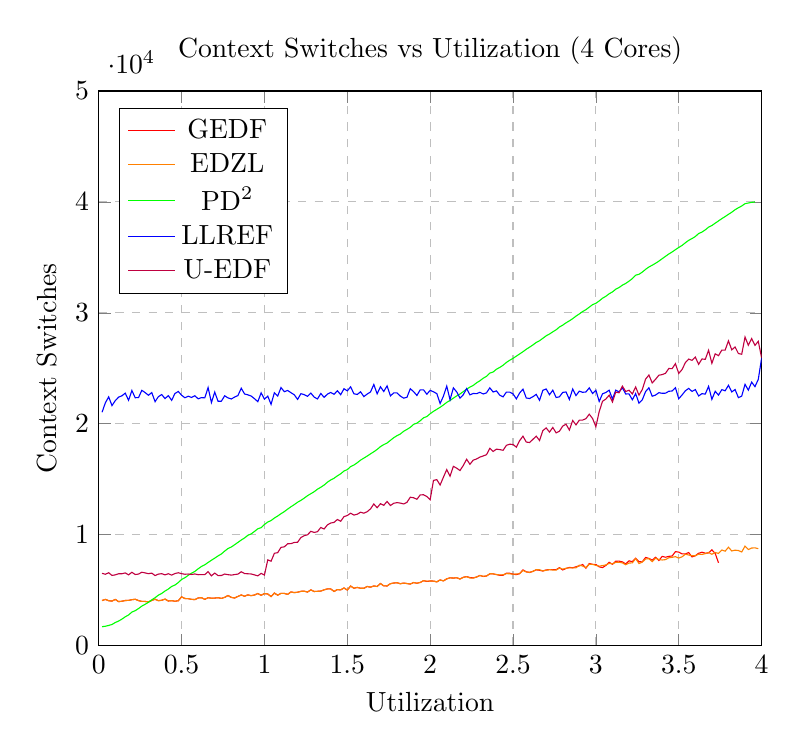
\begin{tikzpicture}
\begin{axis}[
    title={Context Switches vs Utilization (4 Cores)},
    xlabel={Utilization},
    ylabel={Context Switches},
    xmin=0, xmax=4,
    ymin=0, ymax=50000,
    xtick distance=0.5,
    ytick distance=10000,
    legend pos=north west,
    xmajorgrids=true,
    ymajorgrids=true,
    grid style=dashed,
    legend pos=north west,
]
\legend{GEDF, EDZL, PD$^2$, LLREF, U-EDF}
\addplot[color=red]
coordinates {
(0.02,4062.26)(0.04,4161.12)(0.06,4042.44)(0.08,4005.88)(0.1,4155.1)(0.12,3960.68)(0.14,3994.06)(0.16,4061.58)(0.18,4071.6)(0.2,4134.56)(0.22,4170.92)(0.24,4054.44)(0.26,3978.52)(0.28,3976.56)(0.3,3930.22)(0.32,4066.4)(0.34,4174.58)(0.36,4043.1)(0.38,4081.02)(0.4,4188)(0.42,4016.5)(0.44,4046.56)(0.46,3995.06)(0.48,4037.82)(0.5,4390.36)(0.52,4238.92)(0.54,4227.46)(0.56,4164.44)(0.58,4142.68)(0.6,4288.46)(0.62,4313.78)(0.64,4162.76)(0.66,4314.78)(0.68,4263.14)(0.7,4279.12)(0.72,4312.56)(0.74,4250.82)(0.76,4345.36)(0.78,4508.88)(0.8,4340.24)(0.82,4289.12)(0.84,4429.82)(0.86,4558.84)(0.88,4446.22)(0.9,4567.98)(0.92,4495.7)(0.94,4557.5)(0.96,4689.4)(0.98,4536.42)(1,4684.72)(1.02,4648.3)(1.04,4414.44)(1.06,4730.26)(1.08,4539.76)(1.1,4708.8)(1.12,4697.32)(1.14,4617.18)(1.16,4829.7)(1.18,4773.8)(1.2,4807.08)(1.22,4888.64)(1.24,4899.92)(1.26,4824.84)(1.28,5015.86)(1.3,4874.52)(1.32,4888.7)(1.34,4911.08)(1.36,5021.56)(1.38,5106.62)(1.4,5104.08)(1.42,4879)(1.44,5044.8)(1.46,5019.58)(1.48,5188.98)(1.5,5005.36)(1.52,5362.3)(1.54,5169.22)(1.56,5240.38)(1.58,5164.62)(1.6,5167.02)(1.62,5324.58)(1.64,5265.3)(1.66,5369.34)(1.68,5323.24)(1.7,5591.48)(1.72,5374.36)(1.74,5372.66)(1.76,5575.38)(1.78,5635.62)(1.8,5663.06)(1.82,5577.2)(1.84,5632.28)(1.86,5590.78)(1.88,5543.9)(1.9,5680.2)(1.92,5618.3)(1.94,5688.62)(1.96,5848.66)(1.98,5779.12)(2,5816.56)(2.02,5813.5)(2.04,5738.98)(2.06,5914.66)(2.08,5829.48)(2.1,6013)(2.12,6105.49)(2.14,6081.8)(2.16,6113.26)(2.18,5998.94)(2.2,6157.38)(2.22,6214.71)(2.24,6130.15)(2.26,6098.81)(2.28,6177.59)(2.3,6320.11)(2.32,6226.53)(2.34,6271.81)(2.36,6457.45)(2.38,6459.19)(2.4,6400.09)(2.42,6334.59)(2.44,6337.24)(2.46,6521.93)(2.48,6515.14)(2.5,6439.28)(2.52,6393.09)(2.54,6491.06)(2.56,6820.32)(2.58,6649.19)(2.6,6587.93)(2.62,6693.77)(2.64,6822.43)(2.66,6786.67)(2.68,6716.08)(2.7,6820.17)(2.72,6842.24)(2.74,6843.85)(2.76,6838.74)(2.78,7020.66)(2.8,6815.05)(2.82,6951.56)(2.84,7045.05)(2.86,7006.39)(2.88,7102.71)(2.9,7180.17)(2.92,7303.88)(2.94,6975.06)(2.96,7394.81)(2.98,7324)(3,7310.12)(3.02,7094)(3.04,7027.87)(3.06,7220.44)(3.08,7502.77)(3.1,7330.56)(3.12,7600.84)(3.14,7607.21)(3.16,7542.72)(3.18,7361.68)(3.2,7638.44)(3.22,7559.69)(3.24,7869.63)(3.26,7556.27)(3.28,7545.95)(3.3,7941)(3.32,7856.72)(3.34,7698.25)(3.36,7956.95)(3.38,7670)(3.4,8036.92)(3.42,7961.5)(3.44,8039.5)(3.46,8072.86)(3.48,8464.67)(3.5,8423.8)(3.52,8269.14)(3.54,8260.33)(3.56,8384.29)(3.58,7990.5)(3.6,8097.33)(3.62,8317.4)(3.64,8413)(3.66,8327)(3.68,8350.67)(3.7,8629)(3.72,8301)(3.74,7463)
};
\addplot[color=orange]
coordinates {
(0.02,4062.26)(0.04,4161.12)(0.06,4042.44)(0.08,4005.88)(0.1,4155.1)(0.12,3960.68)(0.14,3994.06)(0.16,4061.58)(0.18,4071.6)(0.2,4134.56)(0.22,4170.92)(0.24,4054.44)(0.26,3978.52)(0.28,3976.56)(0.3,3930.22)(0.32,4066.4)(0.34,4174.58)(0.36,4043.1)(0.38,4081.02)(0.4,4188)(0.42,4016.5)(0.44,4046.56)(0.46,3995.06)(0.48,4037.82)(0.5,4390.36)(0.52,4238.92)(0.54,4227.46)(0.56,4164.44)(0.58,4142.68)(0.6,4288.46)(0.62,4313.78)(0.64,4162.76)(0.66,4314.78)(0.68,4263.14)(0.7,4279.12)(0.72,4312.56)(0.74,4250.82)(0.76,4345.36)(0.78,4508.88)(0.8,4340.24)(0.82,4289.12)(0.84,4429.82)(0.86,4558.84)(0.88,4446.22)(0.9,4567.98)(0.92,4495.7)(0.94,4557.5)(0.96,4689.4)(0.98,4536.42)(1,4684.72)(1.02,4648.3)(1.04,4414.44)(1.06,4730.26)(1.08,4539.76)(1.1,4708.8)(1.12,4697.32)(1.14,4617.18)(1.16,4829.7)(1.18,4773.8)(1.2,4807.08)(1.22,4888.64)(1.24,4899.92)(1.26,4824.84)(1.28,5015.86)(1.3,4874.52)(1.32,4888.7)(1.34,4911.08)(1.36,5021.56)(1.38,5106.62)(1.4,5104.08)(1.42,4879)(1.44,5044.8)(1.46,5019.58)(1.48,5188.98)(1.5,5005.36)(1.52,5362.3)(1.54,5169.22)(1.56,5240.38)(1.58,5164.62)(1.6,5167.02)(1.62,5324.58)(1.64,5265.3)(1.66,5369.34)(1.68,5323.24)(1.7,5591.48)(1.72,5374.36)(1.74,5372.66)(1.76,5575.38)(1.78,5635.62)(1.8,5663.06)(1.82,5566.34)(1.84,5632.28)(1.86,5590.78)(1.88,5543.9)(1.9,5680.2)(1.92,5618.3)(1.94,5688.62)(1.96,5848.66)(1.98,5804.96)(2,5816.56)(2.02,5813.5)(2.04,5738.98)(2.06,5914.66)(2.08,5829.48)(2.1,6013)(2.12,6102.1)(2.14,6081.8)(2.16,6113.26)(2.18,5998.94)(2.2,6143.06)(2.22,6209.3)(2.24,6088.3)(2.26,6075.12)(2.28,6174.36)(2.3,6315.54)(2.32,6246.98)(2.34,6270.3)(2.36,6473.56)(2.38,6467.24)(2.4,6394.24)(2.42,6372.28)(2.44,6379.36)(2.46,6483.18)(2.48,6468.36)(2.5,6432.34)(2.52,6451.04)(2.54,6468.94)(2.56,6766.24)(2.58,6630.84)(2.6,6600.88)(2.62,6679.24)(2.64,6846.16)(2.66,6828.3)(2.68,6729.92)(2.7,6783.28)(2.72,6845.5)(2.74,6805.86)(2.76,6801.2)(2.78,6985.76)(2.8,6887.9)(2.82,6968.06)(2.84,7006.76)(2.86,6995.9)(2.88,7009.54)(2.9,7248.84)(2.92,7168.08)(2.94,7029.3)(2.96,7329.64)(2.98,7318.38)(3,7222.96)(3.02,7156.52)(3.04,7208.32)(3.06,7266.38)(3.08,7410.96)(3.1,7358.56)(3.12,7506.98)(3.14,7510.8)(3.16,7450.28)(3.18,7283.68)(3.2,7440.34)(3.22,7451.84)(3.24,7848.62)(3.26,7390.82)(3.28,7521.4)(3.3,7804.18)(3.32,7827.64)(3.34,7563.62)(3.36,7877.74)(3.38,7752.62)(3.4,7713.2)(3.42,7747.58)(3.44,7913.32)(3.46,7952.56)(3.48,8014.74)(3.5,7885.36)(3.52,7999.98)(3.54,8235)(3.56,8163.52)(3.58,8091)(3.6,8097.9)(3.62,8242.3)(3.64,8213.26)(3.66,8286.86)(3.68,8388.38)(3.7,8232.36)(3.72,8389.24)(3.74,8304.22)(3.76,8615.88)(3.78,8505.78)(3.8,8865.14)(3.82,8525.7)(3.84,8598.84)(3.86,8564.82)(3.88,8437.24)(3.9,8963.38)(3.92,8654.94)(3.94,8792.16)(3.96,8808.7)(3.98,8732.48)
};
\addplot[color=green]
coordinates {
(0.02,1695.3)(0.04,1741.6)(0.06,1810.24)(0.08,1900.52)(0.1,2076.04)(0.12,2208.08)(0.14,2382.24)(0.16,2590.74)(0.18,2757.16)(0.2,3014.66)(0.22,3143.52)(0.24,3333.02)(0.26,3554.2)(0.28,3719.7)(0.3,3896.94)(0.32,4117.8)(0.34,4313.02)(0.36,4542.06)(0.38,4700.74)(0.4,4914.32)(0.42,5093.6)(0.44,5326.36)(0.46,5455.8)(0.48,5676.88)(0.5,5955.74)(0.52,6112.62)(0.54,6331.26)(0.56,6521.44)(0.58,6682.64)(0.6,6920.26)(0.62,7128.88)(0.64,7279.02)(0.66,7491.54)(0.68,7690.72)(0.7,7880.24)(0.72,8081.56)(0.74,8255.88)(0.76,8514.56)(0.78,8745.6)(0.8,8885.38)(0.82,9087.38)(0.84,9298)(0.86,9515.2)(0.88,9700.92)(0.9,9939.74)(0.92,10065.9)(0.94,10290)(0.96,10528.1)(0.98,10625.2)(1,10911.6)(1.02,11135.1)(1.04,11268.6)(1.06,11493.9)(1.08,11681.2)(1.1,11887.8)(1.12,12073.9)(1.14,12300.7)(1.16,12512.3)(1.18,12705.8)(1.2,12920.7)(1.22,13088)(1.24,13290.5)(1.26,13511.2)(1.28,13690.7)(1.3,13865.4)(1.32,14096.8)(1.34,14267.7)(1.36,14467.4)(1.38,14724.5)(1.4,14931.7)(1.42,15084.1)(1.44,15298.6)(1.46,15482.3)(1.48,15735.3)(1.5,15859.6)(1.52,16134.1)(1.54,16273.4)(1.56,16480.4)(1.58,16717.4)(1.6,16898.4)(1.62,17083.7)(1.64,17284)(1.66,17469.3)(1.68,17679.7)(1.7,17934.4)(1.72,18114.6)(1.74,18262.9)(1.76,18499.6)(1.78,18733.6)(1.8,18924.9)(1.82,19075)(1.84,19314.3)(1.86,19487.9)(1.88,19668.9)(1.9,19944.2)(1.92,20051.2)(1.94,20267.9)(1.96,20533)(1.98,20644.2)(2,20900.2)(2.02,21111.8)(2.04,21296.2)(2.06,21479.8)(2.08,21689.1)(2.1,21922.1)(2.12,22096.6)(2.14,22304.4)(2.16,22508.7)(2.18,22678.9)(2.2,22892.9)(2.22,23118.1)(2.24,23299.7)(2.26,23451.7)(2.28,23686.8)(2.3,23869.8)(2.32,24099.5)(2.34,24269.6)(2.36,24565.3)(2.38,24658.1)(2.4,24914.6)(2.42,25073.3)(2.44,25275)(2.46,25521.1)(2.48,25718.9)(2.5,25893.4)(2.52,26093.1)(2.54,26291)(2.56,26492.9)(2.58,26708.5)(2.6,26904.8)(2.62,27101)(2.64,27324.9)(2.66,27481.1)(2.68,27700.2)(2.7,27924.5)(2.72,28086.6)(2.74,28282.9)(2.76,28465.3)(2.78,28716.5)(2.8,28887.8)(2.82,29097.5)(2.84,29270)(2.86,29471.1)(2.88,29700.2)(2.9,29894.4)(2.92,30112.5)(2.94,30280.3)(2.96,30510.2)(2.98,30733.3)(3,30855.1)(3.02,31068.9)(3.04,31313.7)(3.06,31484.9)(3.08,31713.4)(3.1,31882.4)(3.12,32125.6)(3.14,32275.6)(3.16,32492.6)(3.18,32647)(3.2,32851.6)(3.22,33082)(3.24,33391.8)(3.26,33470.4)(3.28,33668.2)(3.3,33915.8)(3.32,34128.9)(3.34,34289.3)(3.36,34462.1)(3.38,34656.6)(3.4,34875.7)(3.42,35087.6)(3.44,35302.4)(3.46,35478.4)(3.48,35693.3)(3.5,35886.1)(3.52,36074)(3.54,36312.9)(3.56,36532.8)(3.58,36689.7)(3.6,36874.8)(3.62,37145.4)(3.64,37273.9)(3.66,37472.4)(3.68,37722.9)(3.7,37864.7)(3.72,38080.8)(3.74,38283.8)(3.76,38486.5)(3.78,38679.6)(3.8,38874.8)(3.82,39069.3)(3.84,39294.1)(3.86,39470.6)(3.88,39629.4)(3.9,39838.1)(3.92,39897.5)(3.94,39957.3)(3.96,39993)
};
\addplot[color=blue]
coordinates {
(0.02,21029.7)(0.04,21884.7)(0.06,22420.5)(0.08,21634.7)(0.1,22081.6)(0.12,22396.4)(0.14,22514.6)(0.16,22755.2)(0.18,22110.4)(0.2,22994.7)(0.22,22343.8)(0.24,22348.1)(0.26,23008.9)(0.28,22804)(0.3,22563.8)(0.32,22806.2)(0.34,21989.3)(0.36,22437.6)(0.38,22629.7)(0.4,22271.5)(0.42,22528.2)(0.44,22111.7)(0.46,22722)(0.48,22906.9)(0.5,22568.7)(0.52,22336.5)(0.54,22482.9)(0.56,22366.6)(0.58,22515.3)(0.6,22244.8)(0.62,22350.6)(0.64,22329.7)(0.66,23259.6)(0.68,21902.9)(0.7,22851.5)(0.72,22018.1)(0.74,22029.2)(0.76,22518.2)(0.78,22326.8)(0.8,22227.2)(0.82,22403.6)(0.84,22536.4)(0.86,23199.4)(0.88,22681.1)(0.9,22601)(0.92,22493)(0.94,22253.2)(0.96,21987.8)(0.98,22782.5)(1,22214.6)(1.02,22486)(1.04,21745.9)(1.06,22796.8)(1.08,22493.5)(1.1,23260.4)(1.12,22886.2)(1.14,22998.4)(1.16,22796.6)(1.18,22607.2)(1.2,22191.1)(1.22,22709.1)(1.24,22620.4)(1.26,22473)(1.28,22759.1)(1.3,22398.2)(1.32,22228.9)(1.34,22726.5)(1.36,22375.9)(1.38,22664)(1.4,22816.2)(1.42,22651.3)(1.44,22970.6)(1.46,22613.8)(1.48,23153.6)(1.5,22961)(1.52,23326.8)(1.54,22696.5)(1.56,22637.2)(1.58,22877.4)(1.6,22443.1)(1.62,22673.3)(1.64,22861.3)(1.66,23536)(1.68,22692.5)(1.7,23330.2)(1.72,22904.3)(1.74,23408.3)(1.76,22505.2)(1.78,22774)(1.8,22773.2)(1.82,22492.2)(1.84,22302.8)(1.86,22383.6)(1.88,23155.4)(1.9,22890.6)(1.92,22549.8)(1.94,23054.3)(1.96,23049.7)(1.98,22659)(2,23006.8)(2.02,22876.7)(2.04,22713.6)(2.06,21815.6)(2.08,22486)(2.1,23394)(2.12,22155.5)(2.14,23227.7)(2.16,22869.6)(2.18,22304.5)(2.2,22615.3)(2.22,23169.7)(2.24,22600.2)(2.26,22727)(2.28,22706.9)(2.3,22828.7)(2.32,22681.7)(2.34,22780.8)(2.36,23231.9)(2.38,22858.9)(2.4,22958)(2.42,22570.3)(2.44,22423)(2.46,22851.4)(2.48,22850.5)(2.5,22687.6)(2.52,22237.3)(2.54,22773.2)(2.56,23116.6)(2.58,22316.4)(2.6,22273.1)(2.62,22433.4)(2.64,22647)(2.66,22107.2)(2.68,23013.5)(2.7,23132.8)(2.72,22609.2)(2.74,23024.4)(2.76,22362.6)(2.78,22423)(2.8,22822)(2.82,22862)(2.84,22187.8)(2.86,23129.4)(2.88,22539.5)(2.9,22933.1)(2.92,22831.4)(2.94,22860.1)(2.96,23231.9)(2.98,22727.9)(3,23019.4)(3.02,22006.3)(3.04,22695.1)(3.06,22812)(3.08,23024.5)(3.1,22222.9)(3.12,23026.7)(3.14,22864)(3.16,23240.3)(3.18,22680.8)(3.2,22689.2)(3.22,22156.7)(3.24,22716.1)(3.26,21848.4)(3.28,22151.5)(3.3,22902.6)(3.32,23234.4)(3.34,22475)(3.36,22582.6)(3.38,22795.9)(3.4,22743)(3.42,22751.4)(3.44,22922.5)(3.46,22951.9)(3.48,23247)(3.5,22251.7)(3.52,22591.8)(3.54,22968.1)(3.56,23180.6)(3.58,22910.5)(3.6,23077.3)(3.62,22501.8)(3.64,22708.8)(3.66,22667.4)(3.68,23370.2)(3.7,22198.8)(3.72,22922.9)(3.74,22579.2)(3.76,23072.1)(3.78,22964.8)(3.8,23462)(3.82,22864.6)(3.84,23081.1)(3.86,22347)(3.88,22494.9)(3.9,23547.6)(3.92,23028.4)(3.94,23748.2)(3.96,23341)(3.98,23994.7)(4,25903.8)
};
\addplot[color=purple]
coordinates {
(0.02,6512.16)(0.04,6427.44)(0.06,6563.52)(0.08,6321.84)(0.1,6373.44)(0.12,6470.64)(0.14,6474.72)(0.16,6549.6)(0.18,6373.92)(0.2,6601.68)(0.22,6404.88)(0.24,6441.36)(0.26,6609.36)(0.28,6548.64)(0.3,6478.08)(0.32,6529.44)(0.34,6307.44)(0.36,6442.08)(0.38,6478.32)(0.4,6371.76)(0.42,6475.68)(0.44,6348.48)(0.46,6492)(0.48,6562.08)(0.5,6479.76)(0.52,6428.88)(0.54,6446.88)(0.56,6407.76)(0.58,6456.24)(0.6,6386.4)(0.62,6397.44)(0.64,6394.08)(0.66,6659.76)(0.68,6284.64)(0.7,6532.32)(0.72,6308.1)(0.74,6313.44)(0.76,6445.92)(0.78,6389.04)(0.8,6350.64)(0.82,6401.04)(0.84,6438.96)(0.86,6653.28)(0.88,6491.28)(0.9,6470.4)(0.92,6452.64)(0.94,6369.84)(0.96,6282.24)(0.98,6509.28)(1,6361.2)(1.02,7723.14)(1.04,7604.32)(1.06,8316.88)(1.08,8375.28)(1.1,8852.58)(1.12,8898.92)(1.14,9175.26)(1.16,9188.6)(1.18,9293.06)(1.2,9313.3)(1.22,9736.64)(1.24,9905.88)(1.26,9986.8)(1.28,10297.5)(1.3,10197.4)(1.32,10266.1)(1.34,10644.1)(1.36,10505.2)(1.38,10880.1)(1.4,11047)(1.42,11102.3)(1.44,11365)(1.46,11205.7)(1.48,11619.8)(1.5,11726.5)(1.52,11930.4)(1.54,11761.3)(1.56,11840.3)(1.58,12019.2)(1.6,11933.6)(1.62,12065.8)(1.64,12322.3)(1.66,12761.7)(1.68,12424)(1.7,12786.9)(1.72,12643.9)(1.74,12991.3)(1.76,12623)(1.78,12826.2)(1.8,12885.4)(1.82,12843.4)(1.84,12767.2)(1.86,12913.6)(1.88,13372.6)(1.9,13323.7)(1.92,13186.6)(1.94,13581.5)(1.96,13594.4)(1.98,13430.9)(2,13146)(2.02,14885.7)(2.04,14958.5)(2.06,14472.8)(2.08,15176)(2.1,15865.7)(2.12,15270)(2.14,16157.8)(2.16,15993.3)(2.18,15777.8)(2.2,16237.9)(2.22,16794.2)(2.24,16340.2)(2.26,16716.7)(2.28,16820.8)(2.3,16987.6)(2.32,17092.2)(2.34,17207.3)(2.36,17779.4)(2.38,17500.8)(2.4,17704.7)(2.42,17665.9)(2.44,17602.3)(2.46,18051.4)(2.48,18149.3)(2.5,18131.3)(2.52,17885)(2.54,18474.1)(2.56,18874.2)(2.58,18344.8)(2.6,18304.6)(2.62,18590.5)(2.64,18877.8)(2.66,18485.2)(2.68,19376.8)(2.7,19620.6)(2.72,19243.9)(2.74,19661.4)(2.76,19176.7)(2.78,19322.1)(2.8,19789.8)(2.82,19954.6)(2.84,19428)(2.86,20289.7)(2.88,19896.6)(2.9,20315)(2.92,20329.3)(2.94,20455.3)(2.96,20857.3)(2.98,20467.5)(3,19730.8)(3.02,21090.9)(3.04,22018.6)(3.06,22221.2)(3.08,22568.8)(3.1,21962.5)(3.12,22852.3)(3.14,22788.1)(3.16,23383.1)(3.18,22906.7)(3.2,23014.8)(3.22,22684.9)(3.24,23312.9)(3.26,22571.9)(3.28,23081.2)(3.3,24020.7)(3.32,24388.5)(3.34,23677.9)(3.36,24003.6)(3.38,24370.2)(3.4,24427.8)(3.42,24541.2)(3.44,24976.9)(3.46,24961.4)(3.48,25417.8)(3.5,24531.4)(3.52,24883.3)(3.54,25506.8)(3.56,25826.2)(3.58,25714.5)(3.6,26007)(3.62,25351.9)(3.64,25837)(3.66,25801.7)(3.68,26622.6)(3.7,25447.2)(3.72,26298.2)(3.74,26133.6)(3.76,26639.1)(3.78,26634)(3.8,27469.5)(3.82,26657.8)(3.84,26920.2)(3.86,26325.1)(3.88,26263.5)(3.9,27812.7)(3.92,27072.2)(3.94,27677.3)(3.96,27061.3)(3.98,27430.3)(4,25940.2)
};
\end{axis}
\end{tikzpicture}
}\hspace{1px}
\scalebox{.95}{
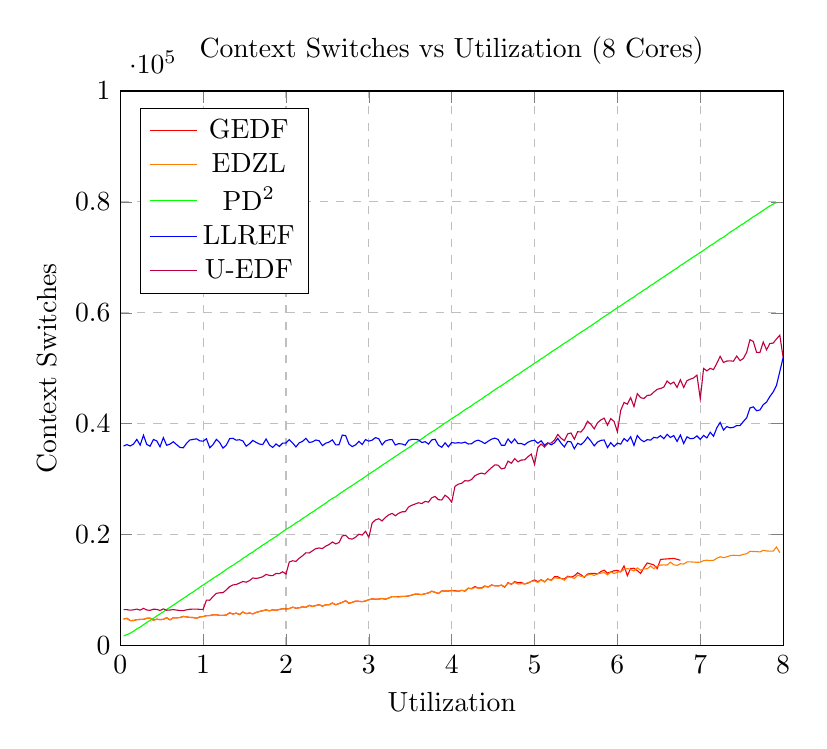
\begin{tikzpicture}
\begin{axis}[
    title={Context Switches vs Utilization (8 Cores)},
    xlabel={Utilization},
    ylabel={Context Switches},
    xmin=0, xmax=8,
    ymin=0, ymax=100000,
    xtick distance=1,
    ytick distance=20000,
    xmajorgrids=true,
    ymajorgrids=true,
    grid style=dashed,
    legend pos=north west,
]
\legend{GEDF, EDZL, PD$^2$, LLREF, U-EDF}
\addplot[color=red]
coordinates {
(0.04,4788.3)(0.08,4909)(0.12,4506.26)(0.16,4511.44)(0.2,4673.5)(0.24,4708.9)(0.28,4727.3)(0.32,4920.7)(0.36,4928.96)(0.4,4584.36)(0.44,4753.26)(0.48,4678.52)(0.52,4728.84)(0.56,5022.94)(0.6,4639.16)(0.64,5016.94)(0.68,5011.54)(0.72,5044.38)(0.76,5240.98)(0.8,5168.9)(0.84,5073.26)(0.88,5059.66)(0.92,4920.52)(0.96,5158.76)(1,5222)(1.04,5395.88)(1.08,5410.76)(1.12,5542.96)(1.16,5543.3)(1.2,5442.24)(1.24,5441.16)(1.28,5515.7)(1.32,5900.2)(1.36,5684.28)(1.4,5854.48)(1.44,5586.16)(1.48,6062.96)(1.52,5748.58)(1.56,5875.4)(1.6,5709.8)(1.64,5981.68)(1.68,6144)(1.72,6277.66)(1.76,6444.02)(1.8,6258.04)(1.84,6449.28)(1.88,6369.32)(1.92,6516.33)(1.96,6632.96)(2,6592.76)(2.04,6665.12)(2.08,6923.68)(2.12,6737.72)(2.16,6803.38)(2.2,6993.24)(2.24,6888.64)(2.28,7249.48)(2.32,7048.94)(2.36,7220.69)(2.4,7369.54)(2.44,7101.52)(2.48,7363.02)(2.52,7363.18)(2.56,7666.77)(2.6,7342.12)(2.64,7568.68)(2.68,7798.45)(2.72,8082.88)(2.76,7617.78)(2.8,7800.9)(2.84,8012.66)(2.88,7980.56)(2.92,7912.08)(2.96,8042.82)(3,8269.61)(3.04,8410.96)(3.08,8358.91)(3.12,8385.42)(3.16,8487.28)(3.2,8355.96)(3.24,8560.94)(3.28,8827.1)(3.32,8834.61)(3.36,8804.88)(3.4,8869.9)(3.44,8855.81)(3.48,8952.28)(3.52,9094.47)(3.56,9281.73)(3.6,9245.13)(3.64,9175.07)(3.68,9348.76)(3.72,9494.85)(3.76,9799.06)(3.8,9598.21)(3.84,9396.42)(3.88,9854.33)(3.92,9832.47)(3.96,9828.8)(4,9931.09)(4.04,9886.79)(4.08,9792.53)(4.12,9948.74)(4.16,9818.23)(4.2,10345.4)(4.24,10271.7)(4.28,10635.3)(4.32,10369.2)(4.36,10392.4)(4.4,10742.2)(4.44,10547.9)(4.48,10934.7)(4.52,10768.5)(4.56,10752.3)(4.6,10885.4)(4.64,10525.6)(4.68,11342.2)(4.72,11050.2)(4.76,11510)(4.8,11344.2)(4.84,11380.8)(4.88,11103.1)(4.92,11257.7)(4.96,11564.5)(5,11841.4)(5.04,11524.9)(5.08,11871)(5.12,11506.1)(5.16,11996.2)(5.2,11764.3)(5.24,12406.8)(5.28,12411.9)(5.32,12075.1)(5.36,12000.5)(5.4,12490.6)(5.44,12337.5)(5.48,12564.6)(5.52,13116.8)(5.56,12770.9)(5.6,12306.7)(5.64,12890.1)(5.68,13014.5)(5.72,13022.9)(5.76,12907.3)(5.8,13332.4)(5.84,13596.6)(5.88,13060.2)(5.92,13284.4)(5.96,13482.5)(6,13550.3)(6.04,13284.3)(6.08,14363)(6.12,12593.3)(6.16,13922.3)(6.2,13931.4)(6.24,13516)(6.28,13009)(6.32,14036)(6.36,14897)(6.44,14541)(6.48,13863)(6.52,15534)(6.68,15715)(6.76,15379)
};
\addplot[color=orange]
coordinates {
(0.04,4788.3)(0.08,4909)(0.12,4506.26)(0.16,4511.44)(0.2,4673.5)(0.24,4708.9)(0.28,4727.3)(0.32,4920.7)(0.36,4928.96)(0.4,4584.36)(0.44,4753.26)(0.48,4678.52)(0.52,4728.84)(0.56,5022.94)(0.6,4639.16)(0.64,5016.94)(0.68,5011.54)(0.72,5044.38)(0.76,5240.98)(0.8,5168.9)(0.84,5073.26)(0.88,5059.66)(0.92,4920.52)(0.96,5158.76)(1,5222)(1.04,5395.88)(1.08,5410.76)(1.12,5542.96)(1.16,5543.3)(1.2,5442.24)(1.24,5441.16)(1.28,5515.7)(1.32,5900.2)(1.36,5684.28)(1.4,5854.48)(1.44,5586.16)(1.48,6062.96)(1.52,5748.58)(1.56,5875.4)(1.6,5709.8)(1.64,5981.68)(1.68,6144)(1.72,6277.66)(1.76,6444.02)(1.8,6258.04)(1.84,6449.28)(1.88,6369.32)(1.92,6506.52)(1.96,6632.96)(2,6592.76)(2.04,6665.12)(2.08,6923.68)(2.12,6737.72)(2.16,6803.38)(2.2,6993.24)(2.24,6888.64)(2.28,7249.48)(2.32,7048.94)(2.36,7216.16)(2.4,7369.54)(2.44,7101.52)(2.48,7363.02)(2.52,7365.72)(2.56,7643.42)(2.6,7388.44)(2.64,7568.68)(2.68,7786.46)(2.72,8072.18)(2.76,7617.78)(2.8,7800.9)(2.84,8012.66)(2.88,7981.34)(2.92,7912.78)(2.96,8042.82)(3,8269.1)(3.04,8410.96)(3.08,8375.34)(3.12,8385.42)(3.16,8463.82)(3.2,8361.18)(3.24,8558.02)(3.28,8827.94)(3.32,8798.26)(3.36,8780.98)(3.4,8835.02)(3.44,8883.52)(3.48,8931.8)(3.52,9117.38)(3.56,9294.06)(3.6,9265.96)(3.64,9215.74)(3.68,9342.1)(3.72,9495.68)(3.76,9799.06)(3.8,9583.04)(3.84,9381.8)(3.88,9813.94)(3.92,9849.86)(3.96,9833.06)(4,9888.14)(4.04,9821.16)(4.08,9798.88)(4.12,9975.22)(4.16,9876.22)(4.2,10339.4)(4.24,10217.8)(4.28,10482)(4.32,10352.7)(4.36,10305.1)(4.4,10649.5)(4.44,10575.5)(4.48,10851.5)(4.52,10804.8)(4.56,10730.1)(4.6,10912.3)(4.64,10636.7)(4.68,11206.7)(4.72,11070.5)(4.76,11373.6)(4.8,11096.5)(4.84,11164.8)(4.88,11136.5)(4.92,11327.9)(4.96,11561.7)(5,11653.4)(5.04,11379.7)(5.08,11867.6)(5.12,11459)(5.16,12057.3)(5.2,11719.2)(5.24,12230.4)(5.28,12142.7)(5.32,12098.6)(5.36,11775.9)(5.4,12373.9)(5.44,12308.6)(5.48,12115.8)(5.52,12672.8)(5.56,12499.7)(5.6,12419.2)(5.64,12722.2)(5.68,12877.2)(5.72,12633.1)(5.76,12948.2)(5.8,13049.3)(5.84,13165.7)(5.88,12749.9)(5.92,13282)(5.96,12997.1)(6,13212.7)(6.04,13354.7)(6.08,13725.7)(6.12,13884.5)(6.16,13703.8)(6.2,13453.6)(6.24,13997.3)(6.28,13593.7)(6.32,13824.6)(6.36,13851)(6.4,14352.1)(6.44,13858.5)(6.48,14352.9)(6.52,14517.6)(6.56,14541.5)(6.6,14519.2)(6.64,15036.8)(6.68,14576.4)(6.72,14453.8)(6.76,14755)(6.8,14694.3)(6.84,15075.2)(6.88,15086.5)(6.92,15051.6)(6.96,15006.7)(7,15051.3)(7.04,15299.5)(7.08,15390)(7.12,15306.2)(7.16,15364.8)(7.2,15736.8)(7.24,16019.4)(7.28,15853.4)(7.32,15992.5)(7.36,16206.1)(7.4,16279.3)(7.44,16260.1)(7.48,16232.1)(7.52,16448.4)(7.56,16549.8)(7.6,16995.9)(7.64,16958.3)(7.68,16941.3)(7.72,16882.3)(7.76,17177.9)(7.8,17061.7)(7.84,17026.3)(7.88,17035.7)(7.92,17773.9)(7.96,16742.3)
};
\addplot[color=green]
coordinates {
(0.04,1737.72)(0.08,1971.9)(0.12,2226.08)(0.16,2582.3)(0.2,3008.86)(0.24,3322.46)(0.28,3754.32)(0.32,4166.64)(0.36,4535.32)(0.4,4893.3)(0.44,5327.28)(0.48,5704.4)(0.52,6083.36)(0.56,6519.84)(0.6,6878.78)(0.64,7294.58)(0.68,7696.6)(0.72,8109.64)(0.76,8489.3)(0.8,8893.28)(0.84,9318.4)(0.88,9674.52)(0.92,10096)(0.96,10506.9)(1,10918)(1.04,11314.9)(1.08,11697.3)(1.12,12105.3)(1.16,12495.1)(1.2,12878.8)(1.24,13299.6)(1.28,13706.9)(1.32,14143.7)(1.36,14465.2)(1.4,14889.1)(1.44,15261.6)(1.48,15711.1)(1.52,16082.9)(1.56,16512.3)(1.6,16854.9)(1.64,17307.1)(1.68,17697.6)(1.72,18118.8)(1.76,18486)(1.8,18906.7)(1.84,19266.3)(1.88,19658.3)(1.92,20096.1)(1.96,20527.4)(2,20928.7)(2.04,21303.3)(2.08,21662.7)(2.12,22130.9)(2.16,22455.7)(2.2,22896.3)(2.24,23264.3)(2.28,23705.5)(2.32,24065.2)(2.36,24481)(2.4,24890.7)(2.44,25286.5)(2.48,25668.7)(2.52,26137.1)(2.56,26531.6)(2.6,26840.1)(2.64,27310.3)(2.68,27705.7)(2.72,28096.5)(2.76,28505.2)(2.8,28866.9)(2.84,29277.4)(2.88,29682.2)(2.92,30064.6)(2.96,30478.7)(3,30907.8)(3.04,31289.2)(3.08,31679.4)(3.12,32088)(3.16,32514.7)(3.2,32884.6)(3.24,33298.2)(3.28,33704.9)(3.32,34086)(3.36,34504.4)(3.4,34892.3)(3.44,35277.9)(3.48,35669.6)(3.52,36072)(3.56,36527)(3.6,36861.7)(3.64,37287.5)(3.68,37704)(3.72,38142.7)(3.76,38509.9)(3.8,38880.4)(3.84,39290.3)(3.88,39704.6)(3.92,40121.2)(3.96,40498.8)(4,40910.5)(4.04,41288.7)(4.08,41683.1)(4.12,42067.5)(4.16,42532.5)(4.2,42859.7)(4.24,43249.5)(4.28,43704.7)(4.32,44073.2)(4.36,44454.5)(4.4,44910.7)(4.44,45276.3)(4.48,45696.1)(4.52,46127.8)(4.56,46503.7)(4.6,46880.4)(4.64,47268.3)(4.68,47715.6)(4.72,48055.1)(4.76,48529.2)(4.8,48870.8)(4.84,49290.8)(4.88,49699.2)(4.92,50081.6)(4.96,50495.5)(5,50898.5)(5.04,51278.1)(5.08,51704.2)(5.12,52064.5)(5.16,52492.1)(5.2,52913.9)(5.24,53307.6)(5.28,53675.1)(5.32,54101.5)(5.36,54496.6)(5.4,54883)(5.44,55274.3)(5.48,55674.6)(5.52,56098.6)(5.56,56501.9)(5.6,56863.6)(5.64,57266.1)(5.68,57649.4)(5.72,58061.4)(5.76,58467)(5.8,58908.2)(5.84,59321.6)(5.88,59676.8)(5.92,60077.1)(5.96,60503)(6,60927.5)(6.04,61273.9)(6.08,61691.3)(6.12,62111.4)(6.16,62495.7)(6.2,62850.4)(6.24,63314.1)(6.28,63672)(6.32,64093.9)(6.36,64455.1)(6.4,64928.1)(6.44,65253.2)(6.48,65700.6)(6.52,66080.3)(6.56,66482.2)(6.6,66900.1)(6.64,67285.5)(6.68,67699)(6.72,68059.7)(6.76,68530.8)(6.8,68882.8)(6.84,69301.2)(6.88,69702.7)(6.92,70094)(6.96,70487.3)(7,70889.7)(7.04,71242.3)(7.08,71696)(7.12,72105.9)(7.16,72446)(7.2,72893.9)(7.24,73312.4)(7.28,73626.5)(7.32,74070.5)(7.36,74530.3)(7.4,74882.6)(7.44,75292.4)(7.48,75714.3)(7.52,76059.7)(7.56,76495)(7.6,76887.2)(7.64,77312.1)(7.68,77668.8)(7.72,78071.7)(7.76,78467.8)(7.8,78878.5)(7.84,79267.5)(7.88,79608)(7.92,79880)
};
\addplot[color=blue]
coordinates {
(0.04,35970.1)(0.08,36236.7)(0.12,35983.6)(0.16,36338.2)(0.2,37175.7)(0.24,36135.3)(0.28,37938.2)(0.32,36262.1)(0.36,35947.5)(0.4,37162)(0.44,36902.7)(0.48,35840.1)(0.52,37487)(0.56,36110.7)(0.6,36321.5)(0.64,36751.3)(0.68,36229)(0.72,35735.4)(0.76,35656.5)(0.8,36458.7)(0.84,37065.4)(0.88,37174.5)(0.92,37276.2)(0.96,36914.7)(1,36850.6)(1.04,37283)(1.08,35669)(1.12,36248.2)(1.16,37174.2)(1.2,36608.5)(1.24,35596.6)(1.28,36146.1)(1.32,37319.8)(1.36,37368.7)(1.4,37030.1)(1.44,37109)(1.48,36899.5)(1.52,35943)(1.56,36396.3)(1.6,36989.3)(1.64,36633)(1.68,36329.7)(1.72,36241.3)(1.76,37253.1)(1.8,36167.8)(1.84,35721.8)(1.88,36352)(1.92,35912.2)(1.96,36505.1)(2,36517.4)(2.04,37140.2)(2.08,36535.6)(2.12,35817)(2.16,36551.4)(2.2,36815.2)(2.24,37367.4)(2.28,36624.8)(2.32,36729.5)(2.36,37066.8)(2.4,36924)(2.44,36052.2)(2.48,36484.7)(2.52,36688.7)(2.56,37084.5)(2.6,36178.7)(2.64,36214.1)(2.68,37954.7)(2.72,37848.8)(2.76,36331)(2.8,35871.4)(2.84,36171.9)(2.88,36820.6)(2.92,36256.2)(2.96,37147)(3,36854.6)(3.04,37039.6)(3.08,37487)(3.12,37288.5)(3.16,36184.2)(3.2,36884.6)(3.24,37091.3)(3.28,37144.3)(3.32,36157)(3.36,36408.6)(3.4,36347.4)(3.44,36136.6)(3.48,37017.8)(3.52,37172.9)(3.56,37182.4)(3.6,37087.2)(3.64,36604.4)(3.68,36762.2)(3.72,36331)(3.76,37089.9)(3.8,37193.3)(3.84,36109.4)(3.88,35751.7)(3.92,36553)(3.96,35833.3)(4,36624.8)(4.04,36495.6)(4.08,36578.6)(4.12,36506.4)(4.16,36686)(4.2,36343.3)(4.24,36392.2)(4.28,36838.3)(4.32,37041)(4.36,36777.1)(4.4,36424.9)(4.44,36845.1)(4.48,37209.6)(4.52,37409.5)(4.56,37163.4)(4.6,36124.3)(4.64,36101.2)(4.68,37250.4)(4.72,36518.7)(4.76,37232.7)(4.8,36418.1)(4.84,36429)(4.88,36176.4)(4.92,36654.7)(4.96,36915.8)(5,37017.8)(5.04,36475.1)(5.08,36918.6)(5.12,36125.7)(5.16,36552.7)(5.2,36195)(5.24,36544)(5.28,37360.6)(5.32,36491.5)(5.36,35823.8)(5.4,36817.9)(5.44,36726.8)(5.48,35477)(5.52,36475.2)(5.56,36207.3)(5.6,36773)(5.64,37595.8)(5.68,36881.8)(5.72,35997.8)(5.76,36683.3)(5.8,36998.8)(5.84,37062.7)(5.88,35697.3)(5.92,36585.4)(5.96,35891.8)(6,36502.5)(6.04,36316.1)(6.08,37329.3)(6.12,36830.2)(6.16,37648.9)(6.2,36083.5)(6.24,37869.2)(6.28,37138.8)(6.32,36749.9)(6.36,37126.6)(6.4,37036.3)(6.44,37545.5)(6.48,37421.1)(6.52,37857.4)(6.56,37293.9)(6.6,38078)(6.64,37521.6)(6.68,37868.1)(6.72,36810.2)(6.76,37965.3)(6.8,36420.7)(6.84,37648.2)(6.88,37298.8)(6.92,37360.7)(6.96,37799.8)(7,37185.4)(7.04,37884.6)(7.08,37445.5)(7.12,38466.4)(7.16,37745)(7.2,39274.6)(7.24,40225.3)(7.28,38850.4)(7.32,39495.3)(7.36,39249.6)(7.4,39349.5)(7.44,39660.1)(7.48,39665.2)(7.52,40401.1)(7.56,41066.3)(7.6,42841.5)(7.64,43041.2)(7.68,42344.3)(7.72,42478.1)(7.76,43429.8)(7.8,43901.6)(7.84,44913)(7.88,45722.3)(7.92,46925.9)(7.96,49409.5)(8,51939.8)
};
\addplot[color=purple]
coordinates {
(0.04,6473.04)(0.08,6471.6)(0.12,6379.92)(0.16,6445.2)(0.2,6573.36)(0.24,6389.76)(0.28,6707.52)(0.32,6414.72)(0.36,6343.68)(0.4,6558)(0.44,6527.04)(0.48,6324.72)(0.52,6615.36)(0.56,6372.48)(0.6,6409.68)(0.64,6485.52)(0.68,6393.36)(0.72,6306.24)(0.76,6292.32)(0.8,6445.92)(0.84,6540.96)(0.88,6571.2)(0.92,6578.16)(0.96,6525.84)(1,6503.04)(1.04,8186.72)(1.08,8177.2)(1.12,8839.92)(1.16,9411.92)(1.2,9516.62)(1.24,9535.1)(1.28,10043.3)(1.32,10625.4)(1.36,10938.7)(1.4,10997.3)(1.44,11280.4)(1.48,11552.6)(1.52,11422)(1.56,11708.6)(1.6,12186.6)(1.64,12105.7)(1.68,12214.3)(1.72,12411.3)(1.76,12833.6)(1.8,12643.7)(1.84,12600.9)(1.88,13003.6)(1.92,12965.8)(1.96,13306.2)(2,12888.5)(2.04,15070.6)(2.08,15285.7)(2.12,15183.2)(2.16,15746.1)(2.2,16196.1)(2.24,16725.3)(2.28,16695.7)(2.32,17081.2)(2.36,17477.5)(2.4,17594.9)(2.44,17484.9)(2.48,17932.6)(2.52,18203.3)(2.56,18675.9)(2.6,18330.3)(2.64,18582.3)(2.68,19768.5)(2.72,19883)(2.76,19290.1)(2.8,19187.3)(2.84,19541)(2.88,20084.2)(2.92,19921.3)(2.96,20603.8)(3,19511.3)(3.04,22096.2)(3.08,22662.1)(3.12,22867.6)(3.16,22473.8)(3.2,23103.9)(3.24,23565)(3.28,23834.2)(3.32,23408.4)(3.36,23843.9)(3.4,24113.7)(3.44,24140.4)(3.48,24991.1)(3.52,25297)(3.56,25529.1)(3.6,25751.7)(3.64,25609.8)(3.68,25998.6)(3.72,25860.5)(3.76,26650.7)(3.8,26889)(3.84,26305.9)(3.88,26248.4)(3.92,27104.6)(3.96,26661.1)(4,25852.8)(4.04,28713.5)(4.08,29101.6)(4.12,29257.2)(4.16,29739.1)(4.2,29659.9)(4.24,29944)(4.28,30615.6)(4.32,30918.1)(4.36,31096.9)(4.4,30915.7)(4.44,31528.8)(4.48,32060.8)(4.52,32575.5)(4.56,32533.2)(4.6,31855)(4.64,31986.9)(4.68,33254)(4.72,32872.7)(4.76,33698.1)(4.8,33132.6)(4.84,33455.4)(4.88,33482.4)(4.92,34044.7)(4.96,34513.3)(5,32662.8)(5.04,35737.2)(5.08,36336.5)(5.12,35795.2)(5.16,36448.6)(5.2,36520.6)(5.24,37034.7)(5.28,38064.2)(5.32,37387.3)(5.36,36943.6)(5.4,38171.5)(5.44,38337.8)(5.48,37219.8)(5.52,38559.8)(5.56,38499.8)(5.6,39239.4)(5.64,40448.4)(5.68,39891.4)(5.72,39075.7)(5.76,40171.1)(5.8,40676.4)(5.84,41002.7)(5.88,39722.8)(5.92,40916.7)(5.96,40399.5)(6,38529.8)(6.04,42402.6)(6.08,43835)(6.12,43525.6)(6.16,44700)(6.2,43095.9)(6.24,45417.9)(6.28,44702.9)(6.32,44542)(6.36,45110.7)(6.4,45155.1)(6.44,45713.2)(6.48,46202.4)(6.52,46350)(6.56,46600.9)(6.6,47702.8)(6.64,47143.3)(6.68,47517.4)(6.72,46546.1)(6.76,47923.4)(6.8,46547.8)(6.84,47773.6)(6.88,48035.6)(6.92,48256.5)(6.96,48763.7)(7,44477.7)(7.04,49962)(7.08,49526.9)(7.12,49978.8)(7.16,49757.7)(7.2,50912.6)(7.24,52139.4)(7.28,51044.3)(7.32,51299.5)(7.36,51338.2)(7.4,51264)(7.44,52203.6)(7.48,51370.9)(7.52,51764)(7.56,52875.2)(7.6,55154.5)(7.64,54825.1)(7.68,52861.4)(7.72,52828.9)(7.76,54737.2)(7.8,53318.3)(7.84,54468.1)(7.88,54534.1)(7.92,55297.3)(7.96,55951.3)(8,51939.8)
};
\end{axis}
\end{tikzpicture}
}
\caption{Context Switches vs Utilization experimental results.}
\label{fig_cswitch}
\end{figure}

\begin{figure}
\scalebox{.95}{
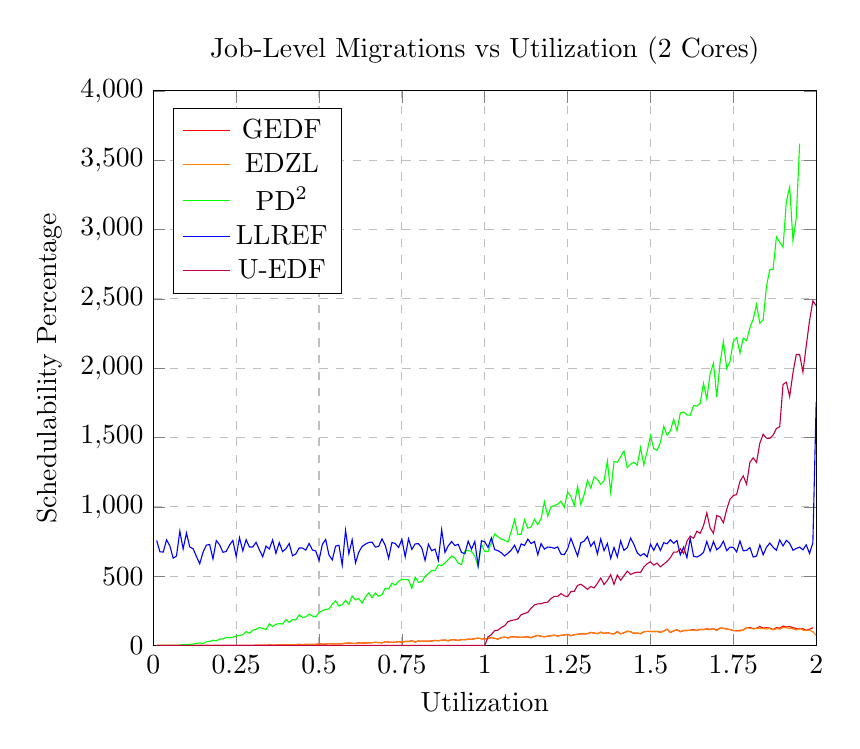
\begin{tikzpicture}
\begin{axis}[
    title={Job-Level Migrations vs Utilization (2 Cores)},
    xlabel={Utilization},
    ylabel={Schedulability Percentage},
    xmin=0, xmax=2,
    ymin=0, ymax=4000,
    xtick distance=0.25,
    ytick distance=500,
    xmajorgrids=true,
    ymajorgrids=true,
    grid style=dashed,
    legend pos=north west,
]
\legend{GEDF, EDZL, PD$^2$, LLREF, U-EDF}
\addplot[color=red]
coordinates {
(0.01,0)(0.02,0)(0.03,0)(0.04,0)(0.05,0)(0.06,0)(0.07,0)(0.08,0)(0.09,0)(0.1,0)(0.11,0)(0.12,0)(0.13,0)(0.14,0)(0.15,0)(0.16,0)(0.17,0)(0.18,0)(0.19,0.02)(0.2,0)(0.21,0.16)(0.22,0.6)(0.23,0.22)(0.24,0.46)(0.25,0.52)(0.26,0.34)(0.27,0.98)(0.28,1.64)(0.29,1.76)(0.3,1.38)(0.31,2.08)(0.32,2.98)(0.33,1.96)(0.34,2.02)(0.35,3.9)(0.36,3.24)(0.37,3.26)(0.38,4.52)(0.39,4.18)(0.4,5.36)(0.41,6.58)(0.42,5.98)(0.43,6.84)(0.44,7.98)(0.45,6.68)(0.46,7.8)(0.47,8.56)(0.48,8.38)(0.49,8.76)(0.5,11.94)(0.51,10.44)(0.52,10.38)(0.53,14.28)(0.54,11.66)(0.55,12.44)(0.56,12.36)(0.57,13.16)(0.58,16.66)(0.59,18.2)(0.6,15.72)(0.61,15)(0.62,19.96)(0.63,18.02)(0.64,18.54)(0.65,19.14)(0.66,20.56)(0.67,23.64)(0.68,21.06)(0.69,20.16)(0.7,26.94)(0.71,25.22)(0.72,23.18)(0.73,23.82)(0.74,28.68)(0.75,23.76)(0.76,29.62)(0.77,29.14)(0.78,34.68)(0.79,25.3)(0.8,32.78)(0.81,31)(0.82,31.76)(0.83,31.56)(0.84,32.82)(0.85,36.6)(0.86,34.52)(0.87,38.94)(0.88,39.74)(0.89,33.84)(0.9,42.34)(0.91,41.1)(0.92,36.7)(0.93,43.48)(0.94,42.06)(0.95,45.44)(0.96,44.86)(0.97,49.84)(0.98,53.42)(0.99,49.12)(1,47.4)(1.01,51.26)(1.02,57.94)(1.03,50.98)(1.04,47.14)(1.05,57.62)(1.06,60.8)(1.07,54.5)(1.08,62.98)(1.09,63.06)(1.1,60.76)(1.11,58.54)(1.12,60.9)(1.13,62.46)(1.14,56.32)(1.15,66.26)(1.16,73.26)(1.17,66.96)(1.18,63.28)(1.19,67.14)(1.2,70.98)(1.21,75.08)(1.22,68.66)(1.23,73.24)(1.24,76.06)(1.25,81.04)(1.26,71.26)(1.27,77.78)(1.28,81.52)(1.29,85.34)(1.3,84.02)(1.31,85.54)(1.32,94.36)(1.33,89.94)(1.34,85.5)(1.35,96.66)(1.36,87.78)(1.37,93.08)(1.38,85.88)(1.39,84.44)(1.4,99.76)(1.41,84.78)(1.42,91.54)(1.43,103.42)(1.44,99.58)(1.45,88.36)(1.46,89.94)(1.47,85)(1.48,99.46)(1.49,102.68)(1.5,100.96)(1.51,101.24)(1.52,101.8)(1.53,96.102)(1.54,104.48)(1.55,118.42)(1.56,93.82)(1.57,106.347)(1.58,113.837)(1.59,99.8571)(1.6,108.26)(1.61,108.54)(1.62,110.531)(1.63,114.652)(1.64,108.8)(1.65,116.245)(1.66,115.66)(1.67,120.596)(1.68,118.021)(1.69,120.9)(1.7,111.106)(1.71,126.333)(1.72,124.44)(1.73,119.265)(1.74,115.792)(1.75,108.542)(1.76,106.146)(1.77,108.778)(1.78,112.913)(1.79,129.178)(1.8,129.889)(1.81,121.66)(1.82,124.689)(1.83,136.9)(1.84,125.22)(1.85,128.722)(1.86,125.927)(1.87,115.7)(1.88,129.31)(1.89,124.821)(1.9,140.371)(1.91,133.762)(1.92,137.233)(1.93,128.444)(1.94,122.9)(1.95,119.538)(1.96,121.731)(1.97,109.947)(1.98,117.85)(1.99,129)
};
\addplot[color=orange]
coordinates {
(0.01,0)(0.02,0)(0.03,0)(0.04,0)(0.05,0)(0.06,0)(0.07,0)(0.08,0)(0.09,0)(0.1,0)(0.11,0)(0.12,0)(0.13,0)(0.14,0)(0.15,0)(0.16,0)(0.17,0)(0.18,0)(0.19,0.02)(0.2,0)(0.21,0.16)(0.22,0.6)(0.23,0.22)(0.24,0.46)(0.25,0.52)(0.26,0.34)(0.27,0.98)(0.28,1.64)(0.29,1.76)(0.3,1.38)(0.31,2.08)(0.32,2.98)(0.33,1.96)(0.34,2.02)(0.35,3.9)(0.36,3.24)(0.37,3.26)(0.38,4.52)(0.39,4.18)(0.4,5.36)(0.41,6.58)(0.42,5.98)(0.43,6.84)(0.44,7.98)(0.45,6.68)(0.46,7.8)(0.47,8.56)(0.48,8.38)(0.49,8.76)(0.5,11.94)(0.51,10.44)(0.52,10.38)(0.53,14.28)(0.54,11.66)(0.55,12.44)(0.56,12.36)(0.57,13.16)(0.58,16.66)(0.59,18.2)(0.6,15.72)(0.61,15)(0.62,19.96)(0.63,18.02)(0.64,18.54)(0.65,19.14)(0.66,20.56)(0.67,23.64)(0.68,21.06)(0.69,20.16)(0.7,26.94)(0.71,25.22)(0.72,23.18)(0.73,23.82)(0.74,28.68)(0.75,23.76)(0.76,29.62)(0.77,29.14)(0.78,34.68)(0.79,25.3)(0.8,32.78)(0.81,31)(0.82,31.76)(0.83,31.56)(0.84,32.82)(0.85,36.6)(0.86,34.52)(0.87,38.94)(0.88,39.74)(0.89,33.84)(0.9,42.34)(0.91,41.1)(0.92,36.7)(0.93,43.48)(0.94,42.06)(0.95,45.44)(0.96,44.86)(0.97,49.84)(0.98,53.42)(0.99,49.12)(1,47.4)(1.01,51.26)(1.02,57.94)(1.03,50.98)(1.04,47.14)(1.05,57.62)(1.06,60.8)(1.07,54.5)(1.08,62.98)(1.09,63.06)(1.1,60.76)(1.11,58.54)(1.12,60.9)(1.13,62.46)(1.14,56.32)(1.15,66.26)(1.16,73.26)(1.17,66.96)(1.18,63.28)(1.19,67.14)(1.2,70.98)(1.21,75.08)(1.22,68.66)(1.23,73.24)(1.24,76.06)(1.25,81.04)(1.26,71.26)(1.27,77.78)(1.28,81.52)(1.29,85.34)(1.3,84.02)(1.31,85.54)(1.32,94.36)(1.33,89.94)(1.34,85.5)(1.35,96.66)(1.36,87.78)(1.37,93.08)(1.38,85.88)(1.39,84.44)(1.4,99.76)(1.41,84.78)(1.42,91.54)(1.43,103.42)(1.44,99.58)(1.45,88.36)(1.46,89.94)(1.47,85)(1.48,99.46)(1.49,102.68)(1.5,100.96)(1.51,101.24)(1.52,101.8)(1.53,94.58)(1.54,104.48)(1.55,118.42)(1.56,93.82)(1.57,105.36)(1.58,113.44)(1.59,100.82)(1.6,108.26)(1.61,108.54)(1.62,109.9)(1.63,111.68)(1.64,108.8)(1.65,115.3)(1.66,115.66)(1.67,116.2)(1.68,115.18)(1.69,120.9)(1.7,107.98)(1.71,125.58)(1.72,124.44)(1.73,118.82)(1.74,115.66)(1.75,107.46)(1.76,106)(1.77,105.18)(1.78,111.22)(1.79,129.72)(1.8,124.42)(1.81,119.76)(1.82,122.2)(1.83,125.54)(1.84,121.7)(1.85,119.44)(1.86,122.56)(1.87,113.48)(1.88,121.5)(1.89,118.52)(1.9,130.72)(1.91,127)(1.92,124.26)(1.93,120.7)(1.94,111.72)(1.95,125.1)(1.96,111.24)(1.97,107.224)(1.98,111.9)(1.99,98.6585)(2,73.5)
};
\addplot[color=green]
coordinates {
(0.01,0)(0.02,0)(0.03,0)(0.04,0)(0.05,0.12)(0.06,1.98)(0.07,1.32)(0.08,3.84)(0.09,7.78)(0.1,6.02)(0.11,8.96)(0.12,10.82)(0.13,15.18)(0.14,18.72)(0.15,15.1)(0.16,27.74)(0.17,29)(0.18,38.44)(0.19,32.96)(0.2,46.58)(0.21,48)(0.22,58.4)(0.23,55.9)(0.24,59.94)(0.25,68.6)(0.26,72.64)(0.27,77.62)(0.28,100.96)(0.29,88.08)(0.3,110.14)(0.31,116.9)(0.32,130.66)(0.33,123.26)(0.34,115.38)(0.35,157.1)(0.36,136.74)(0.37,154.34)(0.38,157.64)(0.39,154.88)(0.4,186.94)(0.41,166.76)(0.42,187.8)(0.43,184.16)(0.44,221.02)(0.45,203.44)(0.46,205.14)(0.47,226.76)(0.48,213.02)(0.49,206.54)(0.5,237.44)(0.51,250.76)(0.52,261.14)(0.53,262.4)(0.54,298.96)(0.55,322.22)(0.56,284.56)(0.57,294.4)(0.58,326.08)(0.59,297.24)(0.6,356.96)(0.61,329.34)(0.62,339.44)(0.63,306.02)(0.64,349.06)(0.65,380)(0.66,344.34)(0.67,378.62)(0.68,355.74)(0.69,366.54)(0.7,414.3)(0.71,407.54)(0.72,450.24)(0.73,435.52)(0.74,463.26)(0.75,476.58)(0.76,476.94)(0.77,472.64)(0.78,413.5)(0.79,494.04)(0.8,455.7)(0.81,460.56)(0.82,499.2)(0.83,519.28)(0.84,541.64)(0.85,540.44)(0.86,582.06)(0.87,574.86)(0.88,596.54)(0.89,620.02)(0.9,645.82)(0.91,631.08)(0.92,593.34)(0.93,584.68)(0.94,680.34)(0.95,686.54)(0.96,678.42)(0.97,645.58)(0.98,568.62)(0.99,731.12)(1,676.56)(1.01,677.66)(1.02,740.58)(1.03,805.18)(1.04,783.32)(1.05,768.24)(1.06,760.08)(1.07,747.24)(1.08,824.62)(1.09,908.94)(1.1,799.76)(1.11,803.06)(1.12,907.34)(1.13,846.28)(1.14,855.6)(1.15,910.58)(1.16,872.32)(1.17,916.48)(1.18,1038.06)(1.19,933.28)(1.2,1002.8)(1.21,1009.66)(1.22,1018.84)(1.23,1041.66)(1.24,997.18)(1.25,1106.66)(1.26,1076.2)(1.27,1009.18)(1.28,1148.52)(1.29,1016.5)(1.3,1089.2)(1.31,1191.64)(1.32,1135.34)(1.33,1215.98)(1.34,1197.1)(1.35,1161.82)(1.36,1188.98)(1.37,1330)(1.38,1105.02)(1.39,1326.34)(1.4,1322.42)(1.41,1360.52)(1.42,1402.86)(1.43,1283.92)(1.44,1307.24)(1.45,1322.22)(1.46,1300.7)(1.47,1428.08)(1.48,1301.86)(1.49,1400.02)(1.5,1514.34)(1.51,1420.48)(1.52,1406.78)(1.53,1464.68)(1.54,1581.6)(1.55,1517.26)(1.56,1548.84)(1.57,1631.76)(1.58,1549.8)(1.59,1677.72)(1.6,1684.7)(1.61,1662.62)(1.62,1661.34)(1.63,1730.08)(1.64,1726.64)(1.65,1747.14)(1.66,1890.58)(1.67,1777.36)(1.68,1962.12)(1.69,2035.9)(1.7,1793.8)(1.71,2038.5)(1.72,2193.36)(1.73,1999.22)(1.74,2048.76)(1.75,2192.24)(1.76,2221.56)(1.77,2109.18)(1.78,2217.22)(1.79,2198.76)(1.8,2292.04)(1.81,2353.4)(1.82,2459.7)(1.83,2324.42)(1.84,2348.68)(1.85,2591.72)(1.86,2710.3)(1.87,2713.96)(1.88,2947.39)(1.89,2909.57)(1.9,2873.47)(1.91,3202.71)(1.92,3306.61)(1.93,2920.5)(1.94,3085.5)(1.95,3620)
};
\addplot[color=blue]
coordinates {
(0.01,757.34)(0.02,676.52)(0.03,673.7)(0.04,762.48)(0.05,718.24)(0.06,629.9)(0.07,646.5)(0.08,824.66)(0.09,696.74)(0.1,812.32)(0.11,710.84)(0.12,698.48)(0.13,643.58)(0.14,589.32)(0.15,672.64)(0.16,724.58)(0.17,728.44)(0.18,625.34)(0.19,757.04)(0.2,726.86)(0.21,672.68)(0.22,678.48)(0.23,725.12)(0.24,758.3)(0.25,643.5)(0.26,778.32)(0.27,682.84)(0.28,763.46)(0.29,710.8)(0.3,710.62)(0.31,744.24)(0.32,690.58)(0.33,640.3)(0.34,716.86)(0.35,696.68)(0.36,761.62)(0.37,665.4)(0.38,742.78)(0.39,677.76)(0.4,697.74)(0.41,735.62)(0.42,647.48)(0.43,660.64)(0.44,703.74)(0.45,703.1)(0.46,688.16)(0.47,736.32)(0.48,689.26)(0.49,682.22)(0.5,614.5)(0.51,729.16)(0.52,765.3)(0.53,652.56)(0.54,617.68)(0.55,716.86)(0.56,723.22)(0.57,580.14)(0.58,830.7)(0.59,661.98)(0.6,763.12)(0.61,595.64)(0.62,673.6)(0.63,715.08)(0.64,731.44)(0.65,743.96)(0.66,745.84)(0.67,710.06)(0.68,715.44)(0.69,769.26)(0.7,720.9)(0.71,628.84)(0.72,743.34)(0.73,735.4)(0.74,707.38)(0.75,766.68)(0.76,639.88)(0.77,769.84)(0.78,693.62)(0.79,733.12)(0.8,734.82)(0.81,704.38)(0.82,613.62)(0.83,731)(0.84,683.94)(0.85,696.12)(0.86,614.86)(0.87,835.48)(0.88,671.58)(0.89,719.12)(0.9,750.42)(0.91,721.1)(0.92,729.94)(0.93,671.52)(0.94,662.66)(0.95,753.32)(0.96,693.88)(0.97,750.88)(0.98,574.52)(0.99,755.76)(1,748.86)(1.01,707.98)(1.02,776.48)(1.03,691.54)(1.04,684.22)(1.05,669.04)(1.06,646.66)(1.07,665.64)(1.08,688.82)(1.09,723.38)(1.1,669.12)(1.11,732.84)(1.12,722.2)(1.13,767.28)(1.14,735.62)(1.15,751.2)(1.16,655.42)(1.17,735.3)(1.18,695.88)(1.19,710.54)(1.2,708.24)(1.21,701.2)(1.22,711.48)(1.23,659.06)(1.24,655.54)(1.25,696.42)(1.26,773.58)(1.27,708.64)(1.28,645.58)(1.29,741.2)(1.3,753.68)(1.31,785.38)(1.32,715.32)(1.33,749.76)(1.34,660.5)(1.35,768.8)(1.36,684.42)(1.37,736.1)(1.38,628.78)(1.39,707.66)(1.4,639.44)(1.41,754.44)(1.42,686.62)(1.43,706.34)(1.44,774.82)(1.45,729.34)(1.46,669.36)(1.47,647.6)(1.48,663.06)(1.49,639.6)(1.5,730.66)(1.51,687.04)(1.52,737.28)(1.53,685.88)(1.54,742.08)(1.55,733.74)(1.56,762.86)(1.57,737.38)(1.58,757.84)(1.59,654.1)(1.6,709.06)(1.61,634.42)(1.62,773.86)(1.63,644.34)(1.64,638.34)(1.65,651.02)(1.66,671.82)(1.67,750.22)(1.68,679.42)(1.69,750.28)(1.7,690.66)(1.71,710.58)(1.72,752.56)(1.73,684.52)(1.74,709.74)(1.75,708.24)(1.76,675.58)(1.77,754.18)(1.78,683.08)(1.79,686.26)(1.8,707.1)(1.81,638.04)(1.82,645.22)(1.83,725.36)(1.84,654.88)(1.85,708.84)(1.86,739.04)(1.87,708.96)(1.88,687.22)(1.89,761.82)(1.9,718.46)(1.91,758.58)(1.92,737.14)(1.93,687.28)(1.94,700.26)(1.95,709.88)(1.96,690.48)(1.97,726.06)(1.98,664.38)(1.99,741.32)(2,1758.02)
};
\addplot[color=purple]
coordinates {
(0.01,0)(0.02,0)(0.03,0)(0.04,0)(0.05,0)(0.06,0)(0.07,0)(0.08,0)(0.09,0)(0.1,0)(0.11,0)(0.12,0)(0.13,0)(0.14,0)(0.15,0)(0.16,0)(0.17,0)(0.18,0)(0.19,0)(0.2,0)(0.21,0)(0.22,0)(0.23,0)(0.24,0)(0.25,0)(0.26,0)(0.27,0)(0.28,0)(0.29,0)(0.3,0)(0.31,0)(0.32,0)(0.33,0)(0.34,0)(0.35,0)(0.36,0)(0.37,0)(0.38,0)(0.39,0)(0.4,0)(0.41,0)(0.42,0)(0.43,0)(0.44,0)(0.45,0)(0.46,0)(0.47,0)(0.48,0)(0.49,0)(0.5,0)(0.51,0)(0.52,0)(0.53,0)(0.54,0)(0.55,0)(0.56,0)(0.57,0)(0.58,0)(0.59,0)(0.6,0)(0.61,0)(0.62,0)(0.63,0)(0.64,0)(0.65,0)(0.66,0)(0.67,0)(0.68,0)(0.69,0)(0.7,0)(0.71,0)(0.72,0)(0.73,0)(0.74,0)(0.75,0)(0.76,0)(0.77,0)(0.78,0)(0.79,0)(0.8,0)(0.81,0)(0.82,0)(0.83,0)(0.84,0)(0.85,0)(0.86,0)(0.87,0)(0.88,0)(0.89,0)(0.9,0)(0.91,0)(0.92,0)(0.93,0)(0.94,0)(0.95,0)(0.96,0)(0.97,0)(0.98,0)(0.99,0)(1,0)(1.01,63.2)(1.02,78.58)(1.03,107.52)(1.04,110.98)(1.05,130.58)(1.06,142.56)(1.07,172.44)(1.08,180.36)(1.09,185.68)(1.1,191.76)(1.11,222.78)(1.12,231.74)(1.13,239.78)(1.14,270.1)(1.15,292.84)(1.16,300.32)(1.17,301.86)(1.18,309.06)(1.19,312.94)(1.2,339.12)(1.21,354.6)(1.22,354.34)(1.23,375.54)(1.24,358.62)(1.25,352.28)(1.26,389.68)(1.27,390.64)(1.28,433.46)(1.29,442.3)(1.3,425.14)(1.31,405.84)(1.32,425.8)(1.33,415.66)(1.34,449.1)(1.35,486.84)(1.36,439.9)(1.37,469.44)(1.38,511.42)(1.39,440.7)(1.4,508.62)(1.41,470.92)(1.42,503.44)(1.43,536.58)(1.44,513.2)(1.45,523.12)(1.46,529.58)(1.47,526.88)(1.48,566.76)(1.49,590.16)(1.5,604.28)(1.51,580.4)(1.52,594.62)(1.53,567.72)(1.54,587.42)(1.55,606.38)(1.56,633.4)(1.57,673.3)(1.58,674.36)(1.59,697.74)(1.6,663.92)(1.61,752.08)(1.62,788.94)(1.63,774.14)(1.64,824.52)(1.65,809.36)(1.66,864.44)(1.67,957.22)(1.68,848.08)(1.69,809.8)(1.7,937.94)(1.71,928.02)(1.72,885.94)(1.73,981.4)(1.74,1055.62)(1.75,1081.42)(1.76,1089.72)(1.77,1184)(1.78,1223.48)(1.79,1163.24)(1.8,1321.9)(1.81,1353.9)(1.82,1320.88)(1.83,1459.56)(1.84,1524.22)(1.85,1495.6)(1.86,1495.02)(1.87,1517.7)(1.88,1565.22)(1.89,1578.18)(1.9,1883.1)(1.91,1899.28)(1.92,1795.7)(1.93,1968.84)(1.94,2099.6)(1.95,2098.8)(1.96,1972.96)(1.97,2162.18)(1.98,2343.98)(1.99,2485.62)(2,2451.8)
};
\end{axis}
\end{tikzpicture}
}\hspace{1px}
\scalebox{.95}{
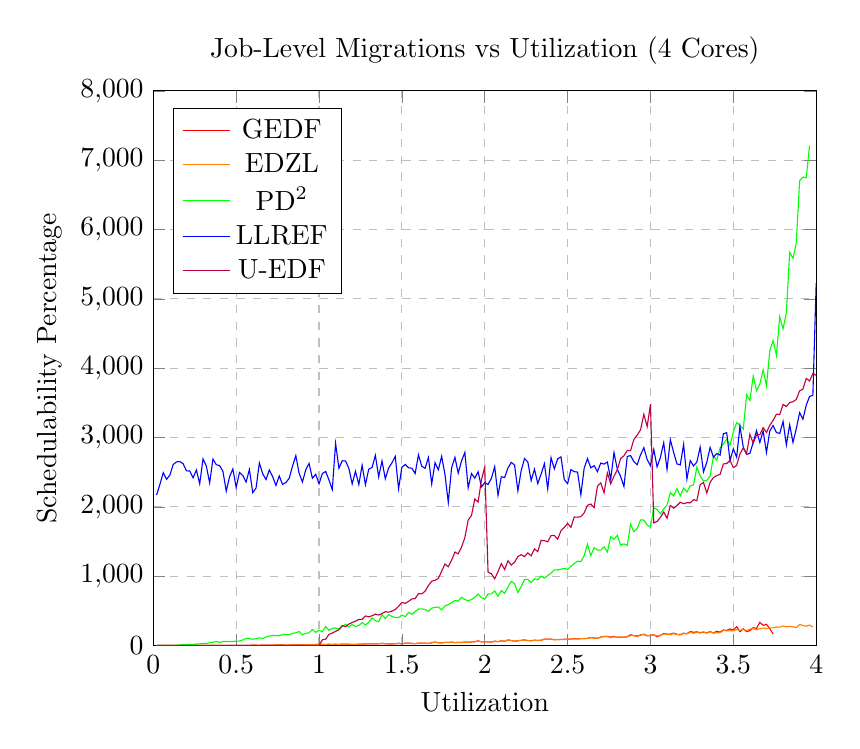
\begin{tikzpicture}
\begin{axis}[
    title={Job-Level Migrations vs Utilization (4 Cores)},
    xlabel={Utilization},
    ylabel={Schedulability Percentage},
    xmin=0, xmax=4,
    ymin=0, ymax=8000,
    xtick distance=0.5,
    ytick distance=1000,
    xmajorgrids=true,
    ymajorgrids=true,
    grid style=dashed,
    legend pos=north west,
]
\legend{GEDF, EDZL, PD$^2$, LLREF, U-EDF}
\addplot[color=red]
coordinates {
(0.02,0)(0.04,0)(0.06,0)(0.08,0)(0.1,0)(0.12,0)(0.14,0)(0.16,0)(0.18,0)(0.2,0)(0.22,0.12)(0.24,0.12)(0.26,0.02)(0.28,0.16)(0.3,0.2)(0.32,0.36)(0.34,0.36)(0.36,0.1)(0.38,0.7)(0.4,2.18)(0.42,1.78)(0.44,1.5)(0.46,2.2)(0.48,1.96)(0.5,2.14)(0.52,3.36)(0.54,1.9)(0.56,2.34)(0.58,2.34)(0.6,4.98)(0.62,4.02)(0.64,2.6)(0.66,6.72)(0.68,5.2)(0.7,3.74)(0.72,5.26)(0.74,7.78)(0.76,7.4)(0.78,7.38)(0.8,6.76)(0.82,6.96)(0.84,8.94)(0.86,9.52)(0.88,9.56)(0.9,9.62)(0.92,10.98)(0.94,12.56)(0.96,9.7)(0.98,14.38)(1,14.58)(1.02,14.88)(1.04,13.92)(1.06,18.58)(1.08,15.72)(1.1,18.76)(1.12,15.46)(1.14,19.52)(1.16,18.12)(1.18,18.7)(1.2,16.56)(1.22,16.88)(1.24,19.46)(1.26,20.78)(1.28,22.98)(1.3,25.34)(1.32,24.5)(1.34,23.6)(1.36,26.58)(1.38,30.76)(1.4,26.02)(1.42,23.08)(1.44,23.04)(1.46,25.2)(1.48,32.84)(1.5,23.28)(1.52,35.86)(1.54,35.5)(1.56,30.34)(1.58,27.06)(1.6,34.8)(1.62,34.7)(1.64,35.9)(1.66,29.76)(1.68,40.04)(1.7,49.7)(1.72,40.72)(1.74,37.24)(1.76,46.24)(1.78,44.3)(1.8,48.92)(1.82,41.551)(1.84,45.8)(1.86,43.26)(1.88,50.26)(1.9,46.54)(1.92,51.56)(1.94,54.74)(1.96,67.06)(1.98,53.102)(2,55.04)(2.02,54.14)(2.04,49.32)(2.06,63.16)(2.08,55.04)(2.1,69.68)(2.12,60.7755)(2.14,81.22)(2.16,72.48)(2.18,62.94)(2.2,69.6458)(2.22,75.4286)(2.24,80.8936)(2.26,71.5417)(2.28,69.551)(2.3,77.5319)(2.32,73.0204)(2.34,75.6383)(2.36,93.617)(2.38,92.5625)(2.4,92.6809)(2.42,85.1522)(2.44,85.3043)(2.46,88.5652)(2.48,90.25)(2.5,89.9787)(2.52,93.9302)(2.54,98.0638)(2.56,95.6596)(2.58,99.9535)(2.6,100.13)(2.62,104.744)(2.64,115.727)(2.66,106.949)(2.68,105.513)(2.7,122.195)(2.72,130.095)(2.74,131.2)(2.76,120.5)(2.78,132.024)(2.8,118.65)(2.82,120.756)(2.84,121.026)(2.86,126.705)(2.88,155.5)(2.9,141.619)(2.92,138.879)(2.94,150.114)(2.96,163.27)(2.98,140.895)(3,146)(3.02,155.743)(3.04,127.1)(3.06,147.296)(3.08,173.767)(3.1,164.519)(3.12,164.162)(3.14,179.265)(3.16,162.034)(3.18,158.368)(3.2,178.074)(3.22,171.188)(3.24,202.037)(3.26,191.045)(3.28,197.727)(3.3,186.143)(3.32,192.556)(3.34,183.583)(3.36,202.25)(3.38,181.1)(3.4,204.917)(3.42,193.75)(3.44,224.6)(3.46,218.143)(3.48,239.5)(3.5,223.6)(3.52,272.143)(3.54,199)(3.56,243.571)(3.58,200.75)(3.6,216.333)(3.62,256.6)(3.64,247.75)(3.66,335.5)(3.68,292)(3.7,306)(3.72,245)(3.74,166)
};
\addplot[color=orange]
coordinates {
(0.02,0)(0.04,0)(0.06,0)(0.08,0)(0.1,0)(0.12,0)(0.14,0)(0.16,0)(0.18,0)(0.2,0)(0.22,0.12)(0.24,0.12)(0.26,0.02)(0.28,0.16)(0.3,0.2)(0.32,0.36)(0.34,0.36)(0.36,0.1)(0.38,0.7)(0.4,2.18)(0.42,1.78)(0.44,1.5)(0.46,2.2)(0.48,1.96)(0.5,2.14)(0.52,3.36)(0.54,1.9)(0.56,2.34)(0.58,2.34)(0.6,4.98)(0.62,4.02)(0.64,2.6)(0.66,6.72)(0.68,5.2)(0.7,3.74)(0.72,5.26)(0.74,7.78)(0.76,7.4)(0.78,7.38)(0.8,6.76)(0.82,6.96)(0.84,8.94)(0.86,9.52)(0.88,9.56)(0.9,9.62)(0.92,10.98)(0.94,12.56)(0.96,9.7)(0.98,14.38)(1,14.58)(1.02,14.88)(1.04,13.92)(1.06,18.58)(1.08,15.72)(1.1,18.76)(1.12,15.46)(1.14,19.52)(1.16,18.12)(1.18,18.7)(1.2,16.56)(1.22,16.88)(1.24,19.46)(1.26,20.78)(1.28,22.98)(1.3,25.34)(1.32,24.5)(1.34,23.6)(1.36,26.58)(1.38,30.76)(1.4,26.02)(1.42,23.08)(1.44,23.04)(1.46,25.2)(1.48,32.84)(1.5,23.28)(1.52,35.86)(1.54,35.5)(1.56,30.34)(1.58,27.06)(1.6,34.8)(1.62,34.7)(1.64,35.9)(1.66,29.76)(1.68,40.04)(1.7,49.7)(1.72,40.72)(1.74,37.24)(1.76,46.24)(1.78,44.3)(1.8,48.92)(1.82,40.86)(1.84,45.8)(1.86,43.26)(1.88,50.26)(1.9,46.54)(1.92,51.56)(1.94,54.74)(1.96,67.06)(1.98,54.36)(2,55.04)(2.02,54.14)(2.04,49.32)(2.06,63.16)(2.08,55.04)(2.1,69.68)(2.12,61.36)(2.14,81.22)(2.16,72.48)(2.18,62.94)(2.2,68.06)(2.22,75.4)(2.24,79.1)(2.26,71.66)(2.28,69.26)(2.3,75.9)(2.32,74.84)(2.34,76.72)(2.36,92.36)(2.38,93.08)(2.4,90.22)(2.42,83.5)(2.44,85.4)(2.46,86.22)(2.48,86.82)(2.5,90.8)(2.52,95)(2.54,96.72)(2.56,94.76)(2.58,98.92)(2.6,101.44)(2.62,99.38)(2.64,116.22)(2.66,107.78)(2.68,105.54)(2.7,120.36)(2.72,132.3)(2.74,130)(2.76,114.98)(2.78,126.7)(2.8,118.66)(2.82,123.72)(2.84,121.42)(2.86,124.32)(2.88,144.02)(2.9,145.92)(2.92,127.66)(2.94,153.9)(2.96,157.4)(2.98,144.92)(3,139.62)(3.02,155.56)(3.04,138.14)(3.06,150.12)(3.08,165.94)(3.1,170.68)(3.12,154.24)(3.14,174.14)(3.16,158.14)(3.18,153.32)(3.2,175.38)(3.22,168.58)(3.24,191.8)(3.26,176.94)(3.28,187.8)(3.3,181.5)(3.32,198.98)(3.34,179.42)(3.36,199.56)(3.38,181.3)(3.4,186.04)(3.42,183.8)(3.44,217.86)(3.46,212)(3.48,212.62)(3.5,213.26)(3.52,229.9)(3.54,219.72)(3.56,238.6)(3.58,212.46)(3.6,237.42)(3.62,245)(3.64,229.14)(3.66,244.7)(3.68,251.94)(3.7,244.08)(3.72,255.3)(3.74,253.98)(3.76,268.6)(3.78,264.82)(3.8,282.62)(3.82,269.96)(3.84,276.26)(3.86,270.72)(3.88,257.94)(3.9,304.36)(3.92,289.551)(3.94,277.689)(3.96,295.326)(3.98,267.655)
};
\addplot[color=green]
coordinates {
(0.02,0)(0.04,0)(0.06,0.24)(0.08,0.12)(0.1,1.88)(0.12,3.3)(0.14,3.54)(0.16,9.64)(0.18,11.96)(0.2,10.92)(0.22,16)(0.24,17.24)(0.26,21.76)(0.28,24.06)(0.3,31.32)(0.32,28.52)(0.34,42.96)(0.36,47.94)(0.38,58.56)(0.4,44.24)(0.42,59.94)(0.44,58.3)(0.46,56)(0.48,58.56)(0.5,63.58)(0.52,65.02)(0.54,80.9)(0.56,103.96)(0.58,100.2)(0.6,90.58)(0.62,98.36)(0.64,111.56)(0.66,100.78)(0.68,124.72)(0.7,138.44)(0.72,145.72)(0.74,144.44)(0.76,140.92)(0.78,159.74)(0.8,158.46)(0.82,156.96)(0.84,173.34)(0.86,185.56)(0.88,201.4)(0.9,155.54)(0.92,175.98)(0.94,182.62)(0.96,231.9)(0.98,190.66)(1,221.44)(1.02,201.94)(1.04,274.18)(1.06,220.3)(1.08,246.16)(1.1,254.64)(1.12,238)(1.14,274.74)(1.16,307.42)(1.18,268.58)(1.2,304)(1.22,276.1)(1.24,287.4)(1.26,331.54)(1.28,296.3)(1.3,336.22)(1.32,398.22)(1.34,358.42)(1.36,343.62)(1.38,443.8)(1.4,391.16)(1.42,445.88)(1.44,420.42)(1.46,404.2)(1.48,404.06)(1.5,438.4)(1.52,417.52)(1.54,477.18)(1.56,451.9)(1.58,489.18)(1.6,527.54)(1.62,528.56)(1.64,520.38)(1.66,491.8)(1.68,539.12)(1.7,550.98)(1.72,555.68)(1.74,515.04)(1.76,571.16)(1.78,591.66)(1.8,618.88)(1.82,652.32)(1.84,641.94)(1.86,697.24)(1.88,664.7)(1.9,645.6)(1.92,663.98)(1.94,695.34)(1.96,743.3)(1.98,691.3)(2,669.44)(2.02,743.52)(2.04,746.5)(2.06,787.04)(2.08,712)(2.1,793.74)(2.12,752.74)(2.14,844.4)(2.16,925.08)(2.18,892.9)(2.2,765.52)(2.22,850.32)(2.24,953.66)(2.26,953.46)(2.28,909.08)(2.3,963.24)(2.32,949.18)(2.34,1001.12)(2.36,974)(2.38,1008.48)(2.4,1045.4)(2.42,1092.16)(2.44,1089.14)(2.46,1102.02)(2.48,1113.22)(2.5,1099.2)(2.52,1143.66)(2.54,1183.2)(2.56,1216.8)(2.58,1211.14)(2.6,1299.12)(2.62,1460.92)(2.64,1296.16)(2.66,1411.74)(2.68,1377.98)(2.7,1376.94)(2.72,1424.2)(2.74,1350.06)(2.76,1569.4)(2.78,1533.64)(2.8,1590.74)(2.82,1448.18)(2.84,1466.92)(2.86,1445.46)(2.88,1748.98)(2.9,1641.16)(2.92,1689.56)(2.94,1812.92)(2.96,1809.94)(2.98,1741.04)(3,1707.28)(3.02,1988.1)(3.04,1961.2)(3.06,1901.8)(3.08,1972.5)(3.1,2027.56)(3.12,2207.38)(3.14,2157.64)(3.16,2264.46)(3.18,2158.38)(3.2,2270.98)(3.22,2215.34)(3.24,2304.52)(3.26,2316.28)(3.28,2574.36)(3.3,2446.42)(3.32,2370.5)(3.34,2384.02)(3.36,2444.28)(3.38,2730.42)(3.4,2674.68)(3.42,2851.46)(3.44,2907.9)(3.46,2977.32)(3.48,2887.08)(3.5,3079.28)(3.52,3216.16)(3.54,3176.6)(3.56,3119.58)(3.58,3619.42)(3.6,3537.06)(3.62,3889.88)(3.64,3679.14)(3.66,3771.28)(3.68,3975.64)(3.7,3746.08)(3.72,4252.74)(3.74,4401.18)(3.76,4187.34)(3.78,4746.38)(3.8,4566.86)(3.82,4798.18)(3.84,5670.88)(3.86,5587.42)(3.88,5807.33)(3.9,6705.45)(3.92,6757.12)(3.94,6748.67)(3.96,7213)
};
\addplot[color=blue]
coordinates {
(0.02,2173.12)(0.04,2325.98)(0.06,2494.06)(0.08,2398.1)(0.1,2459.68)(0.12,2611.42)(0.14,2649.12)(0.16,2654.38)(0.18,2622.94)(0.2,2519.96)(0.22,2517.48)(0.24,2419.96)(0.26,2532.36)(0.28,2333.22)(0.3,2692.62)(0.32,2589.02)(0.34,2345.8)(0.36,2690.62)(0.38,2608.48)(0.4,2596.08)(0.42,2513.1)(0.44,2225.94)(0.46,2434.16)(0.48,2547.56)(0.5,2280.14)(0.52,2495.86)(0.54,2452.06)(0.56,2358.76)(0.58,2540.3)(0.6,2204.94)(0.62,2273.1)(0.64,2634.52)(0.66,2478.34)(0.68,2394.28)(0.7,2532.7)(0.72,2436.22)(0.74,2309.52)(0.76,2446.68)(0.78,2324)(0.8,2351.82)(0.82,2412.5)(0.84,2588.3)(0.86,2739.44)(0.88,2484.52)(0.9,2359.56)(0.92,2535.8)(0.94,2627.8)(0.96,2412.9)(0.98,2470.76)(1,2332.66)(1.02,2481.04)(1.04,2511.58)(1.06,2388.86)(1.08,2248.96)(1.1,2916.96)(1.12,2558)(1.14,2665.34)(1.16,2661.9)(1.18,2555.94)(1.2,2331.56)(1.22,2513.5)(1.24,2320.8)(1.26,2600.22)(1.28,2320.58)(1.3,2544.54)(1.32,2568.9)(1.34,2743.56)(1.36,2433.48)(1.38,2662.46)(1.4,2406.2)(1.42,2561.56)(1.44,2635.58)(1.46,2730)(1.48,2261.24)(1.5,2572.6)(1.52,2611.82)(1.54,2564.78)(1.56,2558.18)(1.58,2481.9)(1.6,2751.48)(1.62,2585.92)(1.64,2556.08)(1.66,2712.42)(1.68,2331.82)(1.7,2638.22)(1.72,2535.4)(1.74,2730.36)(1.76,2466.3)(1.78,2064.44)(1.8,2563.8)(1.82,2714.52)(1.84,2487.24)(1.86,2664.62)(1.88,2785.42)(1.9,2275.54)(1.92,2481.24)(1.94,2414.92)(1.96,2507.06)(1.98,2287.96)(2,2348.68)(2.02,2324.02)(2.04,2410.42)(2.06,2579.78)(2.08,2165.1)(2.1,2435.24)(2.12,2424.06)(2.14,2560.86)(2.16,2642.34)(2.18,2602.82)(2.2,2232.1)(2.22,2525.44)(2.24,2697.22)(2.26,2647.86)(2.28,2379.5)(2.3,2543.62)(2.32,2336.74)(2.34,2473.24)(2.36,2622.74)(2.38,2259.72)(2.4,2710.06)(2.42,2547.82)(2.44,2693.94)(2.46,2721.54)(2.48,2394.14)(2.5,2334.9)(2.52,2538.12)(2.54,2508.4)(2.56,2502.22)(2.58,2173.7)(2.6,2558.88)(2.62,2695.88)(2.64,2562.94)(2.66,2595.02)(2.68,2508.66)(2.7,2632.42)(2.72,2617.24)(2.74,2647.84)(2.76,2397.2)(2.78,2783.44)(2.8,2542.68)(2.82,2437.3)(2.84,2294.94)(2.86,2728.66)(2.88,2740.36)(2.9,2652.38)(2.92,2608.78)(2.94,2749.76)(2.96,2854.24)(2.98,2683.88)(3,2594.5)(3.02,2828.22)(3.04,2577.14)(3.06,2714.58)(3.08,2925.28)(3.1,2539.9)(3.12,2967.8)(3.14,2785)(3.16,2619.5)(3.18,2606.02)(3.2,2900.96)(3.22,2402.7)(3.24,2667.48)(3.26,2591.36)(3.28,2647.2)(3.3,2862.42)(3.32,2504.26)(3.34,2645.54)(3.36,2858.44)(3.38,2715.72)(3.4,2769.9)(3.42,2746.32)(3.44,3055.2)(3.46,3070.28)(3.48,2667.58)(3.5,2837.9)(3.52,2716.62)(3.54,3162.72)(3.56,2861.22)(3.58,2758.5)(3.6,2771.56)(3.62,2929.64)(3.64,3099.3)(3.66,2929.64)(3.68,3095.5)(3.7,2782.72)(3.72,3095.16)(3.74,3172.26)(3.76,3072.54)(3.78,3059.02)(3.8,3233.44)(3.82,2891.88)(3.84,3184.92)(3.86,2931)(3.88,3127.42)(3.9,3358.94)(3.92,3265.44)(3.94,3467.18)(3.96,3592.54)(3.98,3609.78)(4,5227.2)
};
\addplot[color=purple]
coordinates {
(0.02,0)(0.04,0)(0.06,0)(0.08,0)(0.1,0)(0.12,0)(0.14,0)(0.16,0)(0.18,0)(0.2,0)(0.22,0)(0.24,0)(0.26,0)(0.28,0)(0.3,0)(0.32,0)(0.34,0)(0.36,0)(0.38,0)(0.4,0)(0.42,0)(0.44,0)(0.46,0)(0.48,0)(0.5,0)(0.52,0)(0.54,0)(0.56,0)(0.58,0)(0.6,0)(0.62,0)(0.64,0)(0.66,0)(0.68,0)(0.7,0)(0.72,0)(0.74,0)(0.76,0)(0.78,0)(0.8,0)(0.82,0)(0.84,0)(0.86,0)(0.88,0)(0.9,0)(0.92,0)(0.94,0)(0.96,0)(0.98,0)(1,0)(1.02,82.66)(1.04,92.44)(1.06,160.54)(1.08,180.08)(1.1,203.7)(1.12,229.24)(1.14,288.06)(1.16,273.36)(1.18,308.46)(1.2,333.02)(1.22,349.96)(1.24,377.48)(1.26,376.76)(1.28,427.24)(1.3,415)(1.32,429.5)(1.34,453.9)(1.36,439.24)(1.38,461.04)(1.4,488.06)(1.42,481.48)(1.44,496.38)(1.46,520.08)(1.48,564.62)(1.5,622.18)(1.52,607.94)(1.54,636.82)(1.56,672.28)(1.58,677.3)(1.6,747.86)(1.62,745.42)(1.64,783.58)(1.66,864.52)(1.68,929.32)(1.7,940.72)(1.72,968.04)(1.74,1072.4)(1.76,1176.3)(1.78,1136.8)(1.8,1229.9)(1.82,1348.44)(1.84,1323.34)(1.86,1422.02)(1.88,1556.48)(1.9,1810.14)(1.92,1875.82)(1.94,2115.24)(1.96,2069.96)(1.98,2388.46)(2,2577.82)(2.02,1057.16)(2.04,1036.56)(2.06,962.28)(2.08,1066.14)(2.1,1182.14)(2.12,1095.62)(2.14,1223.7)(2.16,1161.48)(2.18,1201.14)(2.2,1283.7)(2.22,1310.04)(2.24,1283.22)(2.26,1335.86)(2.28,1294.82)(2.3,1394.76)(2.32,1354.14)(2.34,1516.28)(2.36,1512.66)(2.38,1496.18)(2.4,1585.92)(2.42,1588.3)(2.44,1533.42)(2.46,1657.12)(2.48,1703.6)(2.5,1763.12)(2.52,1704.92)(2.54,1854.22)(2.56,1851.18)(2.58,1859.62)(2.6,1913.42)(2.62,2023.6)(2.64,2041.4)(2.66,1989.46)(2.68,2299.96)(2.7,2346.78)(2.72,2202.58)(2.74,2491.02)(2.76,2333.42)(2.78,2442.48)(2.8,2536.8)(2.82,2697.16)(2.84,2738.44)(2.86,2813.18)(2.88,2811.64)(2.9,2974.74)(2.92,3037.24)(2.94,3110.64)(2.96,3335.4)(2.98,3158.16)(3,3480.68)(3.02,1769.18)(3.04,1789.6)(3.06,1849.2)(3.08,1926.88)(3.1,1835.44)(3.12,2020.62)(3.14,1981.88)(3.16,2019.66)(3.18,2067.32)(3.2,2046.42)(3.22,2061.16)(3.24,2058.46)(3.26,2105.7)(3.28,2088.52)(3.3,2323.6)(3.32,2350.5)(3.34,2200.56)(3.36,2353.94)(3.38,2423.74)(3.4,2451.46)(3.42,2468.68)(3.44,2619.32)(3.46,2625.46)(3.48,2671.86)(3.5,2566.6)(3.52,2597.22)(3.54,2764.54)(3.56,2849.5)(3.58,2766.78)(3.6,3048.16)(3.62,2919.48)(3.64,3037.12)(3.66,3042.08)(3.68,3143.42)(3.7,3074.6)(3.72,3176.56)(3.74,3246.76)(3.76,3337.14)(3.78,3331.52)(3.8,3478.34)(3.82,3448.22)(3.84,3505.62)(3.86,3516.18)(3.88,3550.92)(3.9,3673.1)(3.92,3697.42)(3.94,3852.54)(3.96,3816.78)(3.98,3922.94)(4,3897.74)
};
\end{axis}
\end{tikzpicture}
}\hspace{1px}
\scalebox{.95}{
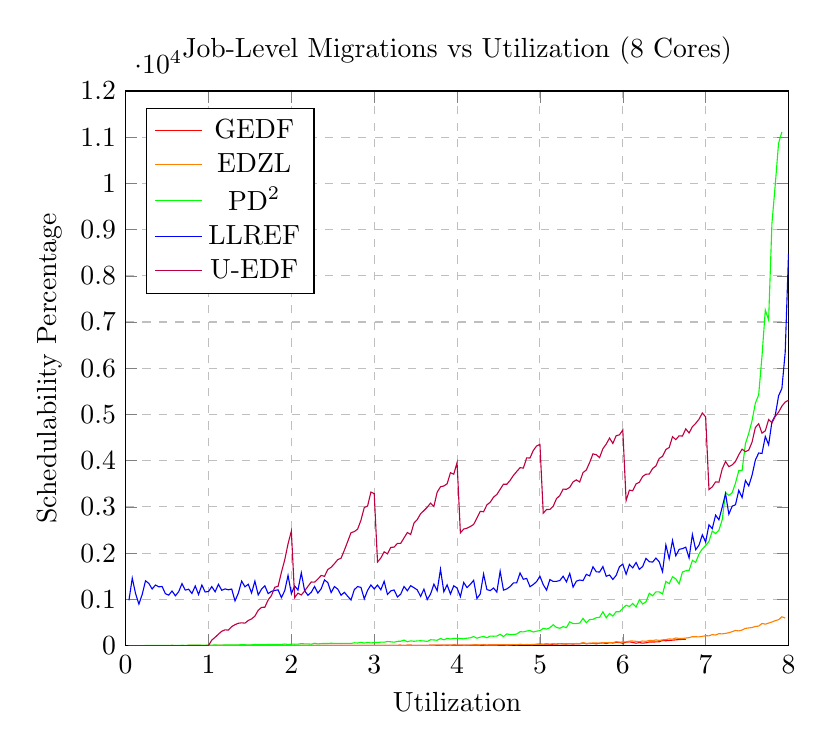
\begin{tikzpicture}
\begin{axis}[
    title={Job-Level Migrations vs Utilization (8 Cores)},
    xlabel={Utilization},
    ylabel={Schedulability Percentage},
    xmin=0, xmax=8,
    ymin=0, ymax=12000,
    xtick distance=1,
    ytick distance=1000,
    xmajorgrids=true,
    ymajorgrids=true,
    grid style=dashed,
    legend pos=north west,
]
\legend{GEDF, EDZL, PD$^2$, LLREF, U-EDF}
\addplot[color=red]
coordinates {
(0.04,0)(0.08,0)(0.12,0)(0.16,0)(0.2,0)(0.24,0)(0.28,0)(0.32,0)(0.36,0)(0.4,0)(0.44,0)(0.48,0.02)(0.52,0.02)(0.56,0.2)(0.6,0.1)(0.64,0.08)(0.68,0.02)(0.72,0.04)(0.76,0.28)(0.8,0.22)(0.84,0.2)(0.88,0.5)(0.92,0.04)(0.96,0.12)(1,0.28)(1.04,0.08)(1.08,0.4)(1.12,0.48)(1.16,0.28)(1.2,0.26)(1.24,0.28)(1.28,0.24)(1.32,0.58)(1.36,0.26)(1.4,0.68)(1.44,0.44)(1.48,0.26)(1.52,0.62)(1.56,0.3)(1.6,0.3)(1.64,0.28)(1.68,0.68)(1.72,0.4)(1.76,0.76)(1.8,0.66)(1.84,0.4)(1.88,0.6)(1.92,0.632653)(1.96,1.14)(2,0.84)(2.04,1.44)(2.08,0.9)(2.12,1.02)(2.16,0.88)(2.2,0.92)(2.24,1.08)(2.28,1.06)(2.32,1.14)(2.36,1.55102)(2.4,2.12)(2.44,1.2)(2.48,1.98)(2.52,1.38776)(2.56,1.29167)(2.6,1.1875)(2.64,1.7)(2.68,2.32653)(2.72,2.5102)(2.76,2.34)(2.8,2.14)(2.84,2.34)(2.88,2.27083)(2.92,1.5102)(2.96,2.32)(3,3.02041)(3.04,2.8)(3.08,4.25532)(3.12,3.44)(3.16,3.80851)(3.2,3.55102)(3.24,3.34043)(3.28,5.28571)(3.32,5.87755)(3.36,3.89583)(3.4,6)(3.44,5.89583)(3.48,5.08696)(3.52,4.87755)(3.56,5.34694)(3.6,4.82979)(3.64,4.35556)(3.68,6.40816)(3.72,7.14894)(3.76,9.28)(3.8,7.68085)(3.84,6.68889)(3.88,8.76087)(3.92,6.53191)(3.96,12.2)(4,10.0682)(4.04,8.71429)(4.08,7.68085)(4.12,6.57143)(4.16,8.825)(4.2,11.2222)(4.24,11.3182)(4.28,9.79487)(4.32,13.6047)(4.36,9.88372)(4.4,12.5854)(4.44,11.4222)(4.48,12.6444)(4.52,15.7073)(4.56,14.975)(4.6,10.9756)(4.64,12.8056)(4.68,21.0357)(4.72,14.6765)(4.76,23.9375)(4.8,19.4412)(4.84,21.2121)(4.88,18.8889)(4.92,18.3939)(4.96,25.6471)(5,33.2414)(5.04,24.875)(5.08,35.2581)(5.12,24.6452)(5.16,30.0357)(5.2,30.8846)(5.24,42.0357)(5.28,35.9048)(5.32,34.0909)(5.36,38.1905)(5.4,33.15)(5.44,39.4762)(5.48,36.4118)(5.52,56.875)(5.56,37.6111)(5.6,44.4167)(5.64,48.3636)(5.68,37)(5.72,50.6154)(5.76,58.8889)(5.8,43.2857)(5.84,63.1333)(5.88,55)(5.92,67.8)(5.96,67)(6,49.3333)(6.04,73)(6.08,80)(6.12,67.6667)(6.16,51)(6.2,64.8571)(6.24,52)(6.28,60)(6.32,77.5)(6.36,76)(6.44,82)(6.48,110)(6.52,104)(6.68,130)(6.76,138)
};
\addplot[color=orange]
coordinates {
(0.04,0)(0.08,0)(0.12,0)(0.16,0)(0.2,0)(0.24,0)(0.28,0)(0.32,0)(0.36,0)(0.4,0)(0.44,0)(0.48,0.02)(0.52,0.02)(0.56,0.2)(0.6,0.1)(0.64,0.08)(0.68,0.02)(0.72,0.04)(0.76,0.28)(0.8,0.22)(0.84,0.2)(0.88,0.5)(0.92,0.04)(0.96,0.12)(1,0.28)(1.04,0.08)(1.08,0.4)(1.12,0.48)(1.16,0.28)(1.2,0.26)(1.24,0.28)(1.28,0.24)(1.32,0.58)(1.36,0.26)(1.4,0.68)(1.44,0.44)(1.48,0.26)(1.52,0.62)(1.56,0.3)(1.6,0.3)(1.64,0.28)(1.68,0.68)(1.72,0.4)(1.76,0.76)(1.8,0.66)(1.84,0.4)(1.88,0.6)(1.92,0.68)(1.96,1.14)(2,0.84)(2.04,1.44)(2.08,0.9)(2.12,1.02)(2.16,0.88)(2.2,0.92)(2.24,1.08)(2.28,1.06)(2.32,1.14)(2.36,1.54)(2.4,2.12)(2.44,1.2)(2.48,1.98)(2.52,1.38)(2.56,1.34)(2.6,1.42)(2.64,1.7)(2.68,2.4)(2.72,2.48)(2.76,2.34)(2.8,2.14)(2.84,2.34)(2.88,2.4)(2.92,1.68)(2.96,2.32)(3,3.02)(3.04,2.8)(3.08,4.4)(3.12,3.44)(3.16,3.88)(3.2,3.64)(3.24,3.76)(3.28,5.52)(3.32,5.78)(3.36,4.14)(3.4,6.14)(3.44,5.86)(3.48,5.1)(3.52,5.02)(3.56,5.46)(3.6,5.06)(3.64,4.38)(3.68,6.46)(3.72,6.94)(3.76,9.28)(3.8,9.24)(3.84,7.26)(3.88,8.56)(3.92,7.4)(3.96,12.74)(4,10.12)(4.04,8.5)(4.08,7.86)(4.12,7.96)(4.16,9.98)(4.2,12.4)(4.24,11.64)(4.28,13.48)(4.32,14)(4.36,10.26)(4.4,13.36)(4.44,11.82)(4.48,12.36)(4.52,16.84)(4.56,15.5)(4.6,12.54)(4.64,14.82)(4.68,21.2)(4.72,17.9)(4.76,22.4)(4.8,20.4)(4.84,22.24)(4.88,20.52)(4.92,25.1)(4.96,27.88)(5,29.8)(5.04,26.1)(5.08,36.42)(5.12,28.84)(5.16,42.56)(5.2,29.82)(5.24,40.54)(5.28,33.3)(5.32,33.74)(5.36,41.1)(5.4,38.9)(5.44,43.64)(5.48,41.9)(5.52,59.68)(5.56,47.7)(5.6,50.34)(5.64,55.34)(5.68,56.5)(5.72,52.02)(5.76,59.62)(5.8,64.44)(5.84,65.42)(5.88,59.46)(5.92,84.62)(5.96,73.6)(6,77.46)(6.04,80.34)(6.08,97.3)(6.12,98.1)(6.16,91.66)(6.2,84.78)(6.24,98.5)(6.28,91.4)(6.32,112.08)(6.36,107.56)(6.4,121.76)(6.44,111.48)(6.48,123.16)(6.52,131.14)(6.56,142.98)(6.6,139.28)(6.64,163.9)(6.68,153.98)(6.72,152.78)(6.76,162.38)(6.8,171.72)(6.84,191.78)(6.88,190.6)(6.92,187.9)(6.96,199.08)(7,213.06)(7.04,210.28)(7.08,237.28)(7.12,227.42)(7.16,257.32)(7.2,252.56)(7.24,264.12)(7.28,277.38)(7.32,301.16)(7.36,326.38)(7.4,317.36)(7.44,335.26)(7.48,372.12)(7.52,381.08)(7.56,390.4)(7.6,412.7)(7.64,421.49)(7.68,477.224)(7.72,463.04)(7.76,486.12)(7.8,509.271)(7.84,538.975)(7.88,559.189)(7.92,622.286)(7.96,596)
};
\addplot[color=green]
coordinates {
(0.04,0)(0.08,0)(0.12,0)(0.16,0)(0.2,0.1)(0.24,0.18)(0.28,0.6)(0.32,1.62)(0.36,1.24)(0.4,1.06)(0.44,1.64)(0.48,2.1)(0.52,1.28)(0.56,2.44)(0.6,2.94)(0.64,3.18)(0.68,6)(0.72,4.96)(0.76,5.64)(0.8,6.1)(0.84,6.56)(0.88,6.16)(0.92,6.12)(0.96,6.5)(1,8.94)(1.04,8.7)(1.08,12.64)(1.12,8.68)(1.16,9.14)(1.2,13.68)(1.24,13.44)(1.28,13.84)(1.32,14.38)(1.36,14.34)(1.4,20.98)(1.44,18.08)(1.48,11.66)(1.52,15.8)(1.56,23.26)(1.6,16.64)(1.64,20.32)(1.68,20.06)(1.72,23.02)(1.76,24.62)(1.8,22.52)(1.84,22.5)(1.88,24.52)(1.92,33.32)(1.96,23.42)(2,30.8)(2.04,29.46)(2.08,30.78)(2.12,41.42)(2.16,36.5)(2.2,36.4)(2.24,29.54)(2.28,49.02)(2.32,36.16)(2.36,42.86)(2.4,44.94)(2.44,45.02)(2.48,50.28)(2.52,46.6)(2.56,47.92)(2.6,45.42)(2.64,46.7)(2.68,47.7)(2.72,45.58)(2.76,59.9)(2.8,55.48)(2.84,70)(2.88,53.96)(2.92,66.9)(2.96,57.46)(3,65.26)(3.04,65.3)(3.08,74.46)(3.12,72.66)(3.16,87.66)(3.2,81.26)(3.24,72.86)(3.28,91.78)(3.32,93.58)(3.36,119.04)(3.4,82.16)(3.44,102.24)(3.48,91.78)(3.52,100.94)(3.56,103.94)(3.6,99.34)(3.64,90.54)(3.68,125.64)(3.72,120.7)(3.76,114.84)(3.8,152.06)(3.84,123.4)(3.88,155.84)(3.92,142.42)(3.96,153.54)(4,156.64)(4.04,150.8)(4.08,145.26)(4.12,160.78)(4.16,166.16)(4.2,194.56)(4.24,158.58)(4.28,182.66)(4.32,196.72)(4.36,169.42)(4.4,203.62)(4.44,202.36)(4.48,205.34)(4.52,244.28)(4.56,193.6)(4.6,252.6)(4.64,237.32)(4.68,237.9)(4.72,250.62)(4.76,299.4)(4.8,296.3)(4.84,314.24)(4.88,323.7)(4.92,293.28)(4.96,312.52)(5,322.62)(5.04,371.3)(5.08,356.76)(5.12,384.34)(5.16,450.36)(5.2,391.94)(5.24,374.08)(5.28,408.6)(5.32,389.42)(5.36,512.98)(5.4,474.58)(5.44,475.8)(5.48,485.56)(5.52,587.1)(5.56,494.66)(5.6,562.6)(5.64,567.78)(5.68,602.12)(5.72,611.44)(5.76,731.48)(5.8,600.66)(5.84,693.9)(5.88,639.36)(5.92,732.86)(5.96,729.86)(6,806.08)(6.04,872.94)(6.08,844.8)(6.12,909.88)(6.16,833.56)(6.2,991.22)(6.24,900.68)(6.28,946.44)(6.32,1131.52)(6.36,1076.94)(6.4,1161.58)(6.44,1160.2)(6.48,1116.96)(6.52,1389.34)(6.56,1338.46)(6.6,1488.62)(6.64,1443.24)(6.68,1335)(6.72,1592.28)(6.76,1617.32)(6.8,1626.98)(6.84,1844.26)(6.88,1800.58)(6.92,1982.36)(6.96,2089.38)(7,2163.58)(7.04,2254.04)(7.08,2477.88)(7.12,2421.8)(7.16,2497.28)(7.2,2723.2)(7.24,3311.92)(7.28,3246.7)(7.32,3307.96)(7.36,3513.3)(7.4,3786.56)(7.44,3788.44)(7.48,4368.94)(7.52,4590.02)(7.56,4865.14)(7.6,5243.12)(7.64,5426.72)(7.68,6262)(7.72,7261.22)(7.76,7042.5)(7.8,9134.38)(7.84,9971.16)(7.88,10867.4)(7.92,11112)
};
\addplot[color=blue]
coordinates {
(0.04,980.46)(0.08,1458.94)(0.12,1123.98)(0.16,897.38)(0.2,1106.62)(0.24,1401.04)(0.28,1343.82)(0.32,1223.6)(0.36,1310.24)(0.4,1271.08)(0.44,1277.94)(0.48,1122.52)(0.52,1091.46)(0.56,1181.04)(0.6,1076.56)(0.64,1165.36)(0.68,1340.1)(0.72,1200.08)(0.76,1218.92)(0.8,1127.3)(0.84,1289.72)(0.88,1104.46)(0.92,1307.76)(0.96,1159.8)(1,1169.16)(1.04,1275.46)(1.08,1163.86)(1.12,1325.32)(1.16,1196.4)(1.2,1226.12)(1.24,1207.24)(1.28,1223.08)(1.32,966.3)(1.36,1133)(1.4,1394.2)(1.44,1271.84)(1.48,1325.92)(1.52,1138.74)(1.56,1394.34)(1.6,1095.56)(1.64,1219.74)(1.68,1292.44)(1.72,1123.86)(1.76,1173.1)(1.8,1192.3)(1.84,1205.46)(1.88,1038.38)(1.92,1186.52)(1.96,1517.94)(2,1125.08)(2.04,1288.48)(2.08,1201.32)(2.12,1573.36)(2.16,1187.52)(2.2,1087.82)(2.24,1152.6)(2.28,1278.84)(2.32,1136.5)(2.36,1228.98)(2.4,1419.92)(2.44,1362.52)(2.48,1146.52)(2.52,1276.18)(2.56,1221.88)(2.6,1088.78)(2.64,1152.4)(2.68,1065.6)(2.72,986.1)(2.76,1210.5)(2.8,1276.92)(2.84,1258.68)(2.88,1010.56)(2.92,1195.16)(2.96,1310.96)(3,1224.7)(3.04,1308.1)(3.08,1206.46)(3.12,1390.68)(3.16,1106.32)(3.2,1181.5)(3.24,1203.4)(3.28,1051.74)(3.32,1112.8)(3.36,1277.66)(3.4,1186.12)(3.44,1296.44)(3.48,1251.34)(3.52,1204.64)(3.56,1062.4)(3.6,1220.56)(3.64,996.68)(3.68,1114.36)(3.72,1327.38)(3.76,1185.58)(3.8,1651.48)(3.84,1164.46)(3.88,1312.58)(3.92,1115.2)(3.96,1293.12)(4,1244.32)(4.04,1058.04)(4.08,1364.84)(4.12,1254.5)(4.16,1325.64)(4.2,1411.18)(4.24,1017.76)(4.28,1118.5)(4.32,1548.56)(4.36,1211.1)(4.4,1189.4)(4.44,1245.22)(4.48,1157.46)(4.52,1609.66)(4.56,1199.64)(4.6,1224.48)(4.64,1276.84)(4.68,1354.72)(4.72,1358.54)(4.76,1569.84)(4.8,1434.72)(4.84,1452.26)(4.88,1272.86)(4.92,1320.12)(4.96,1385.14)(5,1500.5)(5.04,1317.5)(5.08,1198.82)(5.12,1427.34)(5.16,1388.42)(5.2,1389.6)(5.24,1407)(5.28,1500.08)(5.32,1378.94)(5.36,1562.28)(5.4,1263.92)(5.44,1392.54)(5.48,1418.12)(5.52,1404.7)(5.56,1541)(5.6,1507.14)(5.64,1703.86)(5.68,1596.58)(5.72,1589.88)(5.76,1709.82)(5.8,1498.4)(5.84,1527.02)(5.88,1430.64)(5.92,1518)(5.96,1706.36)(6,1762.36)(6.04,1543.98)(6.08,1755.18)(6.12,1681.22)(6.16,1796.4)(6.2,1650.38)(6.24,1711.74)(6.28,1885.94)(6.32,1814.72)(6.36,1805.44)(6.4,1893.18)(6.44,1811.02)(6.48,1598.04)(6.52,2177.46)(6.56,1877.78)(6.6,2274.5)(6.64,1942.24)(6.68,2081.8)(6.72,2097.02)(6.76,2128.68)(6.8,1894.8)(6.84,2403.34)(6.88,2074.06)(6.92,2173.74)(6.96,2395.96)(7,2240.34)(7.04,2612.84)(7.08,2529.16)(7.12,2821.6)(7.16,2720.66)(7.2,2995.8)(7.24,3286.74)(7.28,2843.14)(7.32,3015.5)(7.36,3046.78)(7.4,3357.58)(7.44,3202.98)(7.48,3571.48)(7.52,3454.76)(7.56,3684.96)(7.6,4013.94)(7.64,4166.16)(7.68,4156.44)(7.72,4523.96)(7.76,4345.68)(7.8,4841.46)(7.84,4976.54)(7.88,5403.82)(7.92,5560.88)(7.96,6340.68)(8,8472.98)
};
\addplot[color=purple]
coordinates {
(0.04,0)(0.08,0)(0.12,0)(0.16,0)(0.2,0)(0.24,0)(0.28,0)(0.32,0)(0.36,0)(0.4,0)(0.44,0)(0.48,0)(0.52,0)(0.56,0)(0.6,0)(0.64,0)(0.68,0)(0.72,0)(0.76,0)(0.8,0)(0.84,0)(0.88,0)(0.92,0)(0.96,0)(1,0)(1.04,119.32)(1.08,178.52)(1.12,246.98)(1.16,308.96)(1.2,340.36)(1.24,333.84)(1.28,410.6)(1.32,451.54)(1.36,482.62)(1.4,491.96)(1.44,484.72)(1.48,542.98)(1.52,576.16)(1.56,637.08)(1.6,762.92)(1.64,826.9)(1.68,829.08)(1.72,987.4)(1.76,1081.7)(1.8,1262.02)(1.84,1282.42)(1.88,1584.5)(1.92,1853.52)(1.96,2200.94)(2,2475.22)(2.04,1037.4)(2.08,1134.22)(2.12,1093.46)(2.16,1179.1)(2.2,1281.38)(2.24,1375)(2.28,1371.82)(2.32,1438.34)(2.36,1516.52)(2.4,1498.48)(2.44,1645.28)(2.48,1694.22)(2.52,1772.34)(2.56,1859.78)(2.6,1890.06)(2.64,2063.9)(2.68,2251.14)(2.72,2441.66)(2.76,2465.76)(2.8,2519.84)(2.84,2712.08)(2.88,2986.26)(2.92,3019.36)(2.96,3320.72)(3,3288.36)(3.04,1807.46)(3.08,1894.8)(3.12,2028.52)(3.16,1983.76)(3.2,2124.46)(3.24,2129.46)(3.28,2210.92)(3.32,2212.04)(3.36,2329.62)(3.4,2445.86)(3.44,2402.92)(3.48,2650.52)(3.52,2727.28)(3.56,2853.32)(3.6,2920.1)(3.64,2993.02)(3.68,3082.64)(3.72,3009.74)(3.76,3319.34)(3.8,3435.18)(3.84,3452.7)(3.88,3499.18)(3.92,3739.78)(3.96,3707.24)(4,3958.06)(4.04,2437.82)(4.08,2521.1)(4.12,2539.78)(4.16,2574.7)(4.2,2620.84)(4.24,2760.34)(4.28,2904.68)(4.32,2894.46)(4.36,3044.24)(4.4,3101.04)(4.44,3210.74)(4.48,3268.52)(4.52,3380.36)(4.56,3491.6)(4.6,3489.22)(4.64,3573.48)(4.68,3680.96)(4.72,3766.14)(4.76,3848.78)(4.8,3839.3)(4.84,4060)(4.88,4058.82)(4.92,4221.4)(4.96,4319.02)(5,4352.72)(5.04,2864.64)(5.08,2943.9)(5.12,2945.82)(5.16,3012.5)(5.2,3178.88)(5.24,3246)(5.28,3385.94)(5.32,3380.36)(5.36,3423.52)(5.4,3541.56)(5.44,3585.08)(5.48,3538.2)(5.52,3742.24)(5.56,3799.36)(5.6,3960.56)(5.64,4147.86)(5.68,4128.72)(5.72,4066.74)(5.76,4260.44)(5.8,4357.9)(5.84,4489.9)(5.88,4372.96)(5.92,4540.44)(5.96,4559.64)(6,4662.8)(6.04,3138.72)(6.08,3363.44)(6.12,3349.24)(6.16,3498.22)(6.2,3533.58)(6.24,3659.6)(6.28,3706.58)(6.32,3712.36)(6.36,3830.2)(6.4,3887.02)(6.44,4048.86)(6.48,4094.58)(6.52,4241.76)(6.56,4285.18)(6.6,4518.56)(6.64,4456.48)(6.68,4538.06)(6.72,4532.02)(6.76,4688.46)(6.8,4598.6)(6.84,4736.36)(6.88,4807.56)(6.92,4898.1)(6.96,5031.6)(7,4947.64)(7.04,3376.48)(7.08,3434.28)(7.12,3542)(7.16,3534.74)(7.2,3819.12)(7.24,3983.04)(7.28,3871.38)(7.32,3908.98)(7.36,3982.08)(7.4,4130.26)(7.44,4249.56)(7.48,4194.44)(7.52,4228.74)(7.56,4401.52)(7.6,4718.08)(7.64,4800.04)(7.68,4595.86)(7.72,4646.18)(7.76,4890.24)(7.8,4818.98)(7.84,4957.96)(7.88,5050.24)(7.92,5179.48)(7.96,5268.54)(8,5307.04)
};
\end{axis}
\end{tikzpicture}
}
\caption{Job-Level Migrations vs Utilization experimental results.}
\label{fig_mig}
\end{figure}

% An example of a floating figure using the graphicx package.
% Note that \label must occur AFTER (or within) \caption.
% For figures, \caption should occur after the \includegraphics.
% Note that IEEEtran v1.7 and later has special internal code that
% is designed to preserve the operation of \label within \caption
% even when the captionsoff option is in effect. However, because
% of issues like this, it may be the safest practice to put all your
% \label just after \caption rather than within \caption{}.
%
% Reminder: the "draftcls" or "draftclsnofoot", not "draft", class
% option should be used if it is desired that the figures are to be
% displayed while in draft mode.
%
%\begin{figure}[!t]
%\centering
%\includegraphics[width=2.5in]{myfigure}
% where an .eps filename suffix will be assumed under latex, 
% and a .pdf suffix will be assumed for pdflatex; or what has been declared
% via \DeclareGraphicsExtensions.
%\caption{Simulation results for the network.}
%\label{fig_sim}
%\end{figure}

% Note that the IEEE typically puts floats only at the top, even when this
% results in a large percentage of a column being occupied by floats.


% An example of a double column floating figure using two subfigures.
% (The subfig.sty package must be loaded for this to work.)
% The subfigure \label commands are set within each subfloat command,
% and the \label for the overall figure must come after \caption.
% \hfil is used as a separator to get equal spacing.
% Watch out that the combined width of all the subfigures on a 
% line do not exceed the text width or a line break will occur.
%
%\begin{figure*}[!t]
%\centering
%\subfloat[Case I]{\includegraphics[width=2.5in]{box}%
%\label{fig_first_case}}
%\hfil
%\subfloat[Case II]{\includegraphics[width=2.5in]{box}%
%\label{fig_second_case}}
%\caption{Simulation results for the network.}
%\label{fig_sim}
%\end{figure*}
%
% Note that often IEEE papers with subfigures do not employ subfigure
% captions (using the optional argument to \subfloat[]), but instead will
% reference/describe all of them (a), (b), etc., within the main caption.
% Be aware that for subfig.sty to generate the (a), (b), etc., subfigure
% labels, the optional argument to \subfloat must be present. If a
% subcaption is not desired, just leave its contents blank,
% e.g., \subfloat[].


% An example of a floating table. Note that, for IEEE style tables, the
% \caption command should come BEFORE the table and, given that table
% captions serve much like titles, are usually capitalized except for words
% such as a, an, and, as, at, but, by, for, in, nor, of, on, or, the, to
% and up, which are usually not capitalized unless they are the first or
% last word of the caption. Table text will default to \footnotesize as
% the IEEE normally uses this smaller font for tables.
% The \label must come after \caption as always.
%
%\begin{table}[!t]
%% increase table row spacing, adjust to taste
%\renewcommand{\arraystretch}{1.3}
% if using array.sty, it might be a good idea to tweak the value of
% \extrarowheight as needed to properly center the text within the cells
%\caption{An Example of a Table}
%\label{table_example}
%\centering
%% Some packages, such as MDW tools, offer better commands for making tables
%% than the plain LaTeX2e tabular which is used here.
%\begin{tabular}{|c||c|}
%\hline
%One & Two\\
%\hline
%Three & Four\\
%\hline
%\end{tabular}
%\end{table}


% Note that the IEEE does not put floats in the very first column
% - or typically anywhere on the first page for that matter. Also,
% in-text middle ("here") positioning is typically not used, but it
% is allowed and encouraged for Computer Society conferences (but
% not Computer Society journals). Most IEEE journals/conferences use
% top floats exclusively. 
% Note that, LaTeX2e, unlike IEEE journals/conferences, places
% footnotes above bottom floats. This can be corrected via the
% \fnbelowfloat command of the stfloats package.




\section{Conclusion}
In this paper, we have showcased the features of MARISA as a simulator and visualizer for real-time multiprocessor scheduling, how it compares to other similar tools, and how it can be applied to scheduling algorithm comparisons. While MARISA is still very much a prototype, it showcases the design details and functionality considered for real-time simulation tools, as well as some unique features of MARISA that potentially set it apart from existing tools. With further development, MARISA can support more features shown in other similar tools such as resource access control and synchronization protocols, more scheduling algorithms, better visualizations, more simulation parameters, and live configuration through a user interface.

% conference papers do not normally have an appendix



% use section* for acknowledgment
%\ifCLASSOPTIONcompsoc
  % The Computer Society usually uses the plural form
  %\section*{Acknowledgments}
%\else
  % regular IEEE prefers the singular form
  %\section*{Acknowledgment}
%\fi


%The authors would like to thank...





% trigger a \newpage just before the given reference
% number - used to balance the columns on the last page
% adjust value as needed - may need to be readjusted if
% the document is modified later
%\IEEEtriggeratref{8}
% The "triggered" command can be changed if desired:
%\IEEEtriggercmd{\enlargethispage{-5in}}

% references section

% can use a bibliography generated by BibTeX as a .bbl file
% BibTeX documentation can be easily obtained at:
% http://mirror.ctan.org/biblio/bibtex/contrib/doc/
% The IEEEtran BibTeX style support page is at:
% http://www.michaelshell.org/tex/ieeetran/bibtex/
%\bibliographystyle{IEEEtran}
% argument is your BibTeX string definitions and bibliography database(s)
%\bibliography{IEEEabrv,../bib/paper}
%
% <OR> manually copy in the resultant .bbl file
% set second argument of \begin to the number of references
% (used to reserve space for the reference number labels box)
\newpage
\begin{thebibliography}{1}
\bibitem{cheddar_paper}
F. Singhoff, J. Legrand, L. Nana, and L. Marcé. 2004. Cheddar: a flexible real time scheduling framework. Ada Lett. XXIV, 4 (December 2004), 1–8. https://doi.org/10.1145/1046191.1032298
\bibitem{cheddar_docs}
F. Singhoff, J. Legrand, L. Nana, and L. Marcé. 2004. Cheddar, Project Website,
http://beru.univ-brest.fr/cheddar/
\bibitem{cheddar_repo}
F. Singhoff, J. Legrand, L. Nana, and L. Marcé. 2004. Cheddar, Source Code,
http://beru.univ-brest.fr/svn/CHEDDAR/
\bibitem{yartiss_paper}
Younès Chandarli, Frédéric Fauberteau, Damien Masson, Serge Midonnet, Manar Qamhieh. YARTISS: A Tool to Visualize, Test, Compare and Evaluate Real-Time Scheduling Algorithms. WATERS 2012, Jul 2012, Italy. pp.21--26.
\bibitem{yartiss_docs}
Younès Chandarli, Frédéric Fauberteau, Damien Masson, Serge Midonnet, Manar Qamhieh. YARTISS, Documentation Website, https://igm.univ-mlv.fr/rtalgo/Softwares/YARTISS/doc/
\bibitem{mcrtsim_paper}
J. Wu and Y. -C. Huang, "MCRTsim: A simulation tool for multi-core real-time systems," \emph{2017 International Conference on Applied System Innovation (ICASI)}, Sapporo, Japan, 2017, pp. 461-464, doi: 10.1109/ICASI.2017.7988454.
\bibitem{mcrtsim_repo}
J. Wu and Y. -C. Huang, MCRTsim, GitHub, https://github.com/RESL-NPTU/MCRTsim/tree/master
\bibitem{simso_paper}
Maxime Chéramy, Pierre-Emmanuel Hladik, Anne-Marie Déplanche. SimSo: A Simulation Tool to Evaluate Real-Time Multiprocessor Scheduling Algorithms. 5th International Workshop on Analysis Tools and Methodologies for Embedded and Real-time Systems (WATERS), Jul 2014, Madrid, Spain. 6 p. ⟨hal-01052651⟩
\bibitem{simso_repo}
Maxime Chéramy, Pierre-Emmanuel Hladik, Anne-Marie Déplanche. SimSo, GitHub, https://github.com/MaximeCheramy/simso
\bibitem{ertsim}
Pillai, Anju \& Isha, T.B.. (2013). ERTSim: An embedded real-time task simulator for scheduling. \emph{2013 IEEE International Conference on Computational Intelligence and Computing Research}, IEEE ICCIC 2013. 1-4. 10.1109/ICCIC.2013.6724195. 
\bibitem{edzl}
J. Lee and I. Shin, "EDZL Schedulability Analysis in Real-Time Multicore Scheduling," in \emph{IEEE Transactions on Software Engineering}, vol. 39, no. 7, pp. 910-916, July 2013, doi: 10.1109/TSE.2012.75.
\bibitem{llref}
H. Cho, B. Ravindran and E. D. Jensen, "An Optimal Real-Time Scheduling Algorithm for Multiprocessors," \emph{2006 27th IEEE International Real-Time Systems Symposium (RTSS'06)}, Rio de Janeiro, Brazil, 2006, pp. 101-110, doi: 10.1109/RTSS.2006.10.
\bibitem{pd2}
Anand Srinivasan and James H. Anderson. 2002. "Optimal rate-based scheduling on multiprocessors", in \emph{Proceedings of the thirty-fourth annual ACM symposium on Theory of computing (STOC '02)}, Association for Computing Machinery, New York, NY, USA, pp. 189–198, https://doi.org/10.1145/509907.509938.
\bibitem{run}
P. Regnier, G. Lima, E. Massa, G. Levin and S. Brandt, "RUN: Optimal Multiprocessor Real-Time Scheduling via Reduction to Uniprocessor", 2011 IEEE 32nd Real-Time Systems Symposium, Vienna, Austria, 2011, pp. 104-115, doi: 10.1109/RTSS.2011.17.
\bibitem{uunifast}
Bini, E., Buttazzo, G.C. Measuring the Performance of Schedulability Tests. Real-Time Syst 30, 129–154 (2005). https://doi.org/10.1007/s11241-005-0507-9
\bibitem{randfixedsum}
Emberson, P. \& Stafford, R. \& Davis, R.I.. (2010). Techniques For The Synthesis Of Multiprocessor Tasksets. WATERS'10.
\bibitem{dirichlet}
Frigyik, Andrew Béla, Amol Kapila and Maya R. Gupta, “Introduction to the Dirichlet Distribution and Related Processes.” (2010).
\bibitem{uedf}
G. Nelissen, V. Berten, V. Nélis, J. Goossens and D. Milojevic, "U-EDF: An Unfair But Optimal Multiprocessor Scheduling Algorithm for Sporadic Tasks," \emph{2012 24th Euromicro Conference on Real-Time Systems}, Pisa, Italy, 2012, pp. 13-23, doi: 10.1109/ECRTS.2012.36.
\bibitem{leung}
Joseph Y.-T. Leung, M.L. Merrill, A note on preemptive scheduling of periodic, real-time tasks, Information Processing Letters, Volume 11, Issue 3, 1980, Pages 115-118, ISSN 0020-0190, https://doi.org/10.1016/0020-0190(80)90123-4.
\end{thebibliography}




% that's all folks
\end{document}


